%---Document Class---%
\documentclass[12pt]{book}

%---Packages---%
\usepackage[utf8]{inputenc} %Danish letters
\usepackage{authblk} %Title
\usepackage{graphicx}
\usepackage{sectsty}w
\usepackage{mathcomp}
\usepackage{caption}
\usepackage{subcaption}
\usepackage{listings}
\usepackage{setspace}
\usepackage{mathtools}  %Equations
\usepackage{amsmath}    %Align equations
\usepackage[usenames,dvipsnames]{xcolor}
\usepackage[hidelinks]{hyperref} %Emails in Title
\usepackage[toc,page]{appendix}
\usepackage{multicol}
\usepackage{pdfpages}
\usepackage{wrapfig}
\usepackage{hhline}
\usepackage{tablefootnote}
\usepackage{multirow}
\usepackage{todonotes}
\usepackage{gensymb}

%--- Miscellaneous ---%
\DeclarePairedDelimiter{\abs}{\lvert}{\rvert} %Use of \abs from mathtools

%---Colors---%
\definecolor{chapterColor}{HTML}{004685}
\definecolor{sectionColor}{HTML}{087D9C}
\definecolor{subSectionColor}{HTML}{07928A}
\definecolor{defaultColor}{HTML}{222222}

\chapterfont{\color{chapterColor}}
\sectionfont{\color{sectionColor}}
\subsectionfont{\color{subSectionColor}}
\color{defaultColor}

%---Fonts---%
\usepackage{iwona}
%\usepackage[default]{raleway}
%\usepackage{inconsolata}
\usepackage[T1]{fontenc}
\renewcommand\textbullet{\ensuremath{\bullet}}

%---Page Setup---%
\usepackage[a4paper, margin=2.5cm]{geometry}
\setlength{\parindent}{0em}
\setlength{\parskip}{1em}

%--- Listing ---%
\lstdefinestyle{customc}{
    belowcaptionskip=1\baselineskip,
    breaklines=true,
    xleftmargin=\parindent,
    language=C,
    showstringspaces=false,
    basicstyle=\footnotesize\ttfamily,
    keywordstyle=\bfseries\color{green!40!NavyBlue},
    commentstyle=\itshape\color{purple!40!NavyBlue},
    identifierstyle=\color{black},
    stringstyle=\color{orange},
    tabsize=4,
    numbers=left,
    numberstyle=\tiny\color{gray},
}
\lstset{style=customc}

%--- Bibliography ---%
\usepackage[backend=bibtex ,bibencoding=ascii]{biblatex}
\addbibresource{chapters/cha_bibliography/bibliography.bib}
\nocite{*}

%---Title---%
\newcommand{\documentTitle}{Design, simulation and construction of RuBi, a bipedal platform for human-like locomotion studies}
\newcommand{\documentType}{Master Thesis}

\newcommand{\institute}{University of Southern Denmark}
\newcommand{\department}{Faculty of Engineering}
\newcommand{\program}{MSc in Engineering, Robot Systems}

\newcommand{\authorOne}{Jorge Rodriguez Marin}
\newcommand{\authorTwo}{Ignacio Torroba Balmori}

%---Document---%
\begin{document}
    \frontmatter
    %!TEX root = ../../report.tex

% Title Page
\begin{titlepage}

	\begin{center}
	
\includegraphics[width=80mm,keepaspectratio]{figures/sdu_black}\\

	\vspace{0.3cm}
	\textbf{\institute}\\

	\textmd{\department}\\
	\textmd{\program}  %- \textmd{\course}
	\makebox[0pt][l]{
		\hspace{-14cm}
	  \raisebox{-\totalheight-7mm}[0pt][0pt]{
	  	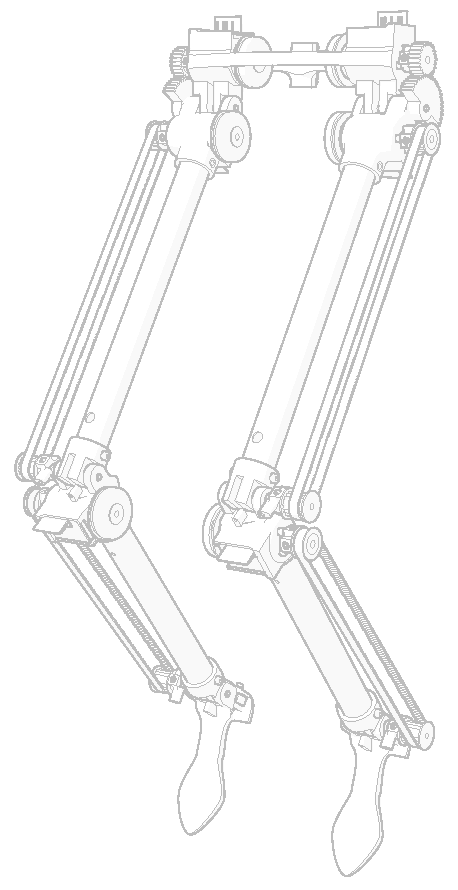
\includegraphics[height=180mm]{figures/legs_technical_drawing.pdf}
	  }
	}\\[4cm]

	\vspace{0.4cm}
	{\huge \bfseries \documentTitle}
	\\
	\vspace{0.5cm}
	{\Large \documentType}
	\\[2cm]

	\begin{tabular}{c}
	 \makebox[4cm]{\emph{Authors}} \\
	 \makebox[4cm]{\authorOne} \\
	 \makebox[4cm]{\authorTwo} \\
	\end{tabular}

	\begin{tabular}{c}
	 \makebox[4cm]{\emph{Supervisors}} \\
	 \makebox[4cm]{\supervisorOne} \\
	 \makebox[4cm]{\supervisorTwo} \\
	\end{tabular}

	\vfill
	{\large \today}
	\end{center}

\end{titlepage}

    %!TEX root = ../../report.tex
%\thispagestyle{empty}
    \null\vspace{\stretch {1}}
        \begin{flushright}
                This is the Dedication.
        \end{flushright}
\vspace{\stretch{2}}\null
    %!TEX root = ../../report.tex
\newenvironment{abstract}%
    {\null\vfill\begin{center}%
    \bfseries Abstract\end{center}}%
    {\vfill\null}
        \begin{abstract}
        The modern field of robotics, in its attempt to understand and mimic the underlying principles of legged locomotion, has in the past decades given birth to some of the most advanced existing bipedal creatures, finding inspiration in nature and the human being.
        This thesis contributes the biped robot RuBi and its development environment to the advancement of this area of the engineering.
        RuBi is a human-inspired, compliance-reconfigurable and low-cost bipedal platform for research in human-like walking and running gaits control.
        The framework presented consists of the lower body frame of the robot and ROS enabled control architecture, a simulation model and environment and a test bench for 2D motion.
        The controller interface with the robot and the simulation environment in Gazebo has been successfully implemented tested.
        A set of experiments for the robot prototype is presented here although they have not been conducted due to time constraints and eventualities.
        Furthermore, everything has been set so that the utilization of the framework can be easily learned and mastered by new users.
        \end{abstract} 
    %!TEX root = ../../report.tex
\newenvironment{resumen}%
    {\null\vfill\begin{center}%
    \bfseries Resumen\end{center}}%
    {\vfill\null}
        \begin{resumen}
        El moderno campo de la robótica, en su intento por comprender e imitar los mecanismos que dan lugar a la locomoción bípeda, ha alumbrado en las últimas décadas a algunas de las criaturas bípedas más avanzadas, inspirándose en la naturaleza y el ser humano.
        Este proyecto de master quiere aportar a esta línea de investigación en ingeniería el robot bípedo RuBi y su entorno de desarrollo.
        RuBi es un robot de proporciones humanas, bajo coste y amortiguación regulable en las articulaciones concebido para la investigación en el control y generación de distintos tipos de locomoción bípedo.
        Conforman el conjunto de intrumentos creado las piernas del robot hasta la cadera, su sistema de control basado en ROS, su modelo de simulación en Gazebo y un banco de pruebas para desplazamientos en 2D.
        La interfaz con los controladores del robot y su entorno de simulación ha sido implementada y testeada con éxito.
        Además, se han diseñado varios experimentos para el prototipo del robot, aunque no han podido llevarse a cabo debido a los e imprevistos retrasos sufridos.
        Por último, todo ha sido debidamente documentado para facilitar a los futuros usuarios el uso del proyecto.
        \end{resumen}
    %!TEX root = ../../report.tex
\newenvironment{acknowledgements}%
    {\null\vfill\begin{center}%
    \bfseries Acknowledgements\end{center}}%
    {\vfill\null}
        \begin{acknowledgements}
        The completion of a Master Thesis entails an amount of devotion and effort difficult to assess since its extension is not bounded to a single semester of actual work, but it comprises the process of acquisition of all the skills and knowledge applied on it.
        Thus, the task of properly acknowledging all those who somehow contributed to this moment turns out to be non-trivial.\\ 
        We have tried our best here.\\
        Our most sincere gratitude goes to our thesis supervisors Jørgen Christian Larsen and Poramate Manoonpong. 
        Their support and advice have let us write this page today.\\
        To our families correspond an embarrassingly big percentage of the credit for this thesis and all that has come before. Their unconditional encouragement and love made us find ourselves in Denmark, doing what we have always liked and being just happy.\\
        And finally, a grateful word for our friends and classmates, here and there.
        You made the whole path worth walking, guys.
        \end{acknowledgements}
    \singlespacing
    \tableofcontents
    \listoftables
    \listoffigures

    \mainmatter
    %!TEX root = ../../report.tex
\chapter{Introduction}
\label{chap:introduction}

%!TEX root = ../../../report.tex

\section{Overall description}
\label{sec:overall_description}
The present thesis aims at laying the foundations of the construction of a robust, low-cost and reconfigurable bipedal locomotion platform for human-like walking and running gait generation and control studies. 
The idea behind this project is to contribute to the on-going line of research in locomotion control at the AI department at the Maersk Mc-Kinney Møller Institute with a new biped robot for further investigation.

The devise, construction and testing of a functional robot of this complexity is by definition a task of great magnitude that involves the conjunction of several disciplines within the robotics field, including electromechanics, structural design, materials science and computer science and control, among others.
Such a complex and extended work, together with the time constraints imposed, have made the authors of the project conceive its development with the view in a further growth beyond the scope of a single master thesis.
With this idea in mind, one of the goals aimed here was to carry out the project facilitating to the farthest possible extent the continuity of its development by new students and researchers. 
Hence, both the hardware and software tools utilized and developed have been thought to be as general-purpose as possible, and all the necessary information required to replicate the work performed has been carefully documented here.

With the above explained as guidelines for the whole process the mechanical design of the robot has been carried out striving for simplicity and functionality, for which 3D-print manufacturing has been applied in order to speed up the prototyping, reduce costs and ease the testing.
The conception of the structure is based on standard human parameters with the purpose of mimicking the dynamics of human legs and approximating the final results as much as possible to the gaits performed by people.
The existing software for simulation and control of bipedal robots has been migrated to ROS \cite{ros} and Gazebo \cite{gazebo} to give a bigger portability and generality to the application, and the developed controllers and interfaces are ROS-based as well. 
The electronics hardware utilized in this thesis consists mainly in components developed for the Locokit project \cite{locokit} created at the University of Southern Denmark, which have been adapted to the specific requirements of the task.
Furthermore, in an early stage of the project the platform was meant to be actuated by an existing, although extended, neural control and therefore it has been designed in accordance to its characteristics.
%!TEX root = ../../../report.tex
\section{Goals}
\label{sec:goals}
The objectives of the research and mechatronics work this thesis has implied are detailed below.
Due to the ambitious scope of the project and the wide range of tasks involved it was hard to assess at the initial proposal the time needed and therefore the main goals of the thesis. 

\subsubsection{The Running Bipedal robot RuBi} % (fold)
\label{ssub:the_running_bipedal_robot_rubi}
The robot RuBi has been devised as a platform to be used for testing new control algorithms used for the generation of human-like walking and running gaits and the transition between them.
Therefore, it has to count on a reliable hardware structure able to offer all the needed functionalities, together with a robust software frame capable of dealing with the requirements of such algorithms\footnote{The capabilities that walking and running gaits generation requires are detailed in \ref{sec:bipedal_walking_and_running_gaits}.}.
% subsubsection the_running_bipedal_robot_rubi (end)


\subsubsection{RuBi as a study framework} % (fold)
\label{ssub:rubi_as_a_study_framework}
This thesis aimed at creating not only the robot described below, but a whole framework for legged locomotion studies.
To do so, some more tools besides a first prototype of the robot were targeted as goals, and are listed in \ref{list:goals}.
Some of them have emerged from the actual process of design and construction of the robot, and others have been included with the view on its future use for research.

\begin{itemize}
\label{list:goals}
\item A more general simulation environment than the existing one, based on ROS and Gazebo and eliminating dependencies with LPZ robots, together with a fully-scalable simulation model of the robot. Furthermore, the implementation of the ROS Control set of packages \cite{ros_control} in the system allows for a simple implementation of controllers that can be easily interfaces with Gazebo or the actual robot. This has been tested with two custom controllers.
\item A test bench designed to hold the robot limiting its movements to the motion plane under study and guaranteeing its stability over a treadmill for locomotion experimentation. 
\item A mathematical framework to be used for computation of both kinematic and dynamic parameters and potentially for developing classical controllers from the dynamics model of the robot.
\item An easy to modify and extend software interface with the electronic hardware, aimed at providing a simple and functional control of the robot.
\end{itemize}

Even thought some of these goals have not been fully accomplished in the sense that they still need some improvement to be fully functional, as explained before all the necessary steps to ease the continuity of their development have been taken.
Furthermore, in the original description of the project was also stated that, if possible, some experiments would be devised and carried out in order to test the functionality and physical properties of the prototype. 
However, some eventualities detailed in the next chapters have prevented the project from reaching that stage and a more complex experimentation phase besides the simple tests of functionality are left as further work.
% subsubsection rubi_as_a_study_framework (end)

%!TEX root = ../../../report.tex
\section{Project management} % (fold)
\label{sec:project_management}
The methodology used for this project is Agile.
Agile approaches help teams respond to unpredictability through incremental, iterative work cadences, known as sprints.
It has been implemented as SCRUM \cite{singh2008u} by considering both supervisors as the product managers and having a self managed team striving to build properly tested product increments within short iterations.
By having weekly meetings, empirical feedback has been received closing the iteration circle faster and more concisely.

The tool Trello \cite{trello} has been used in order to keep track of the tasks in the backlog.
Trello is an online project management application and it was used since its design made it similar to post-it notes for management.
It also has the advantage of being online and therefore accessible from both home and workplace through smart phones or computers.
Figure \ref{fig:trello} shows a screen capture of Trello board for a sprint log.

\begin{figure}[ht]
  \centering
  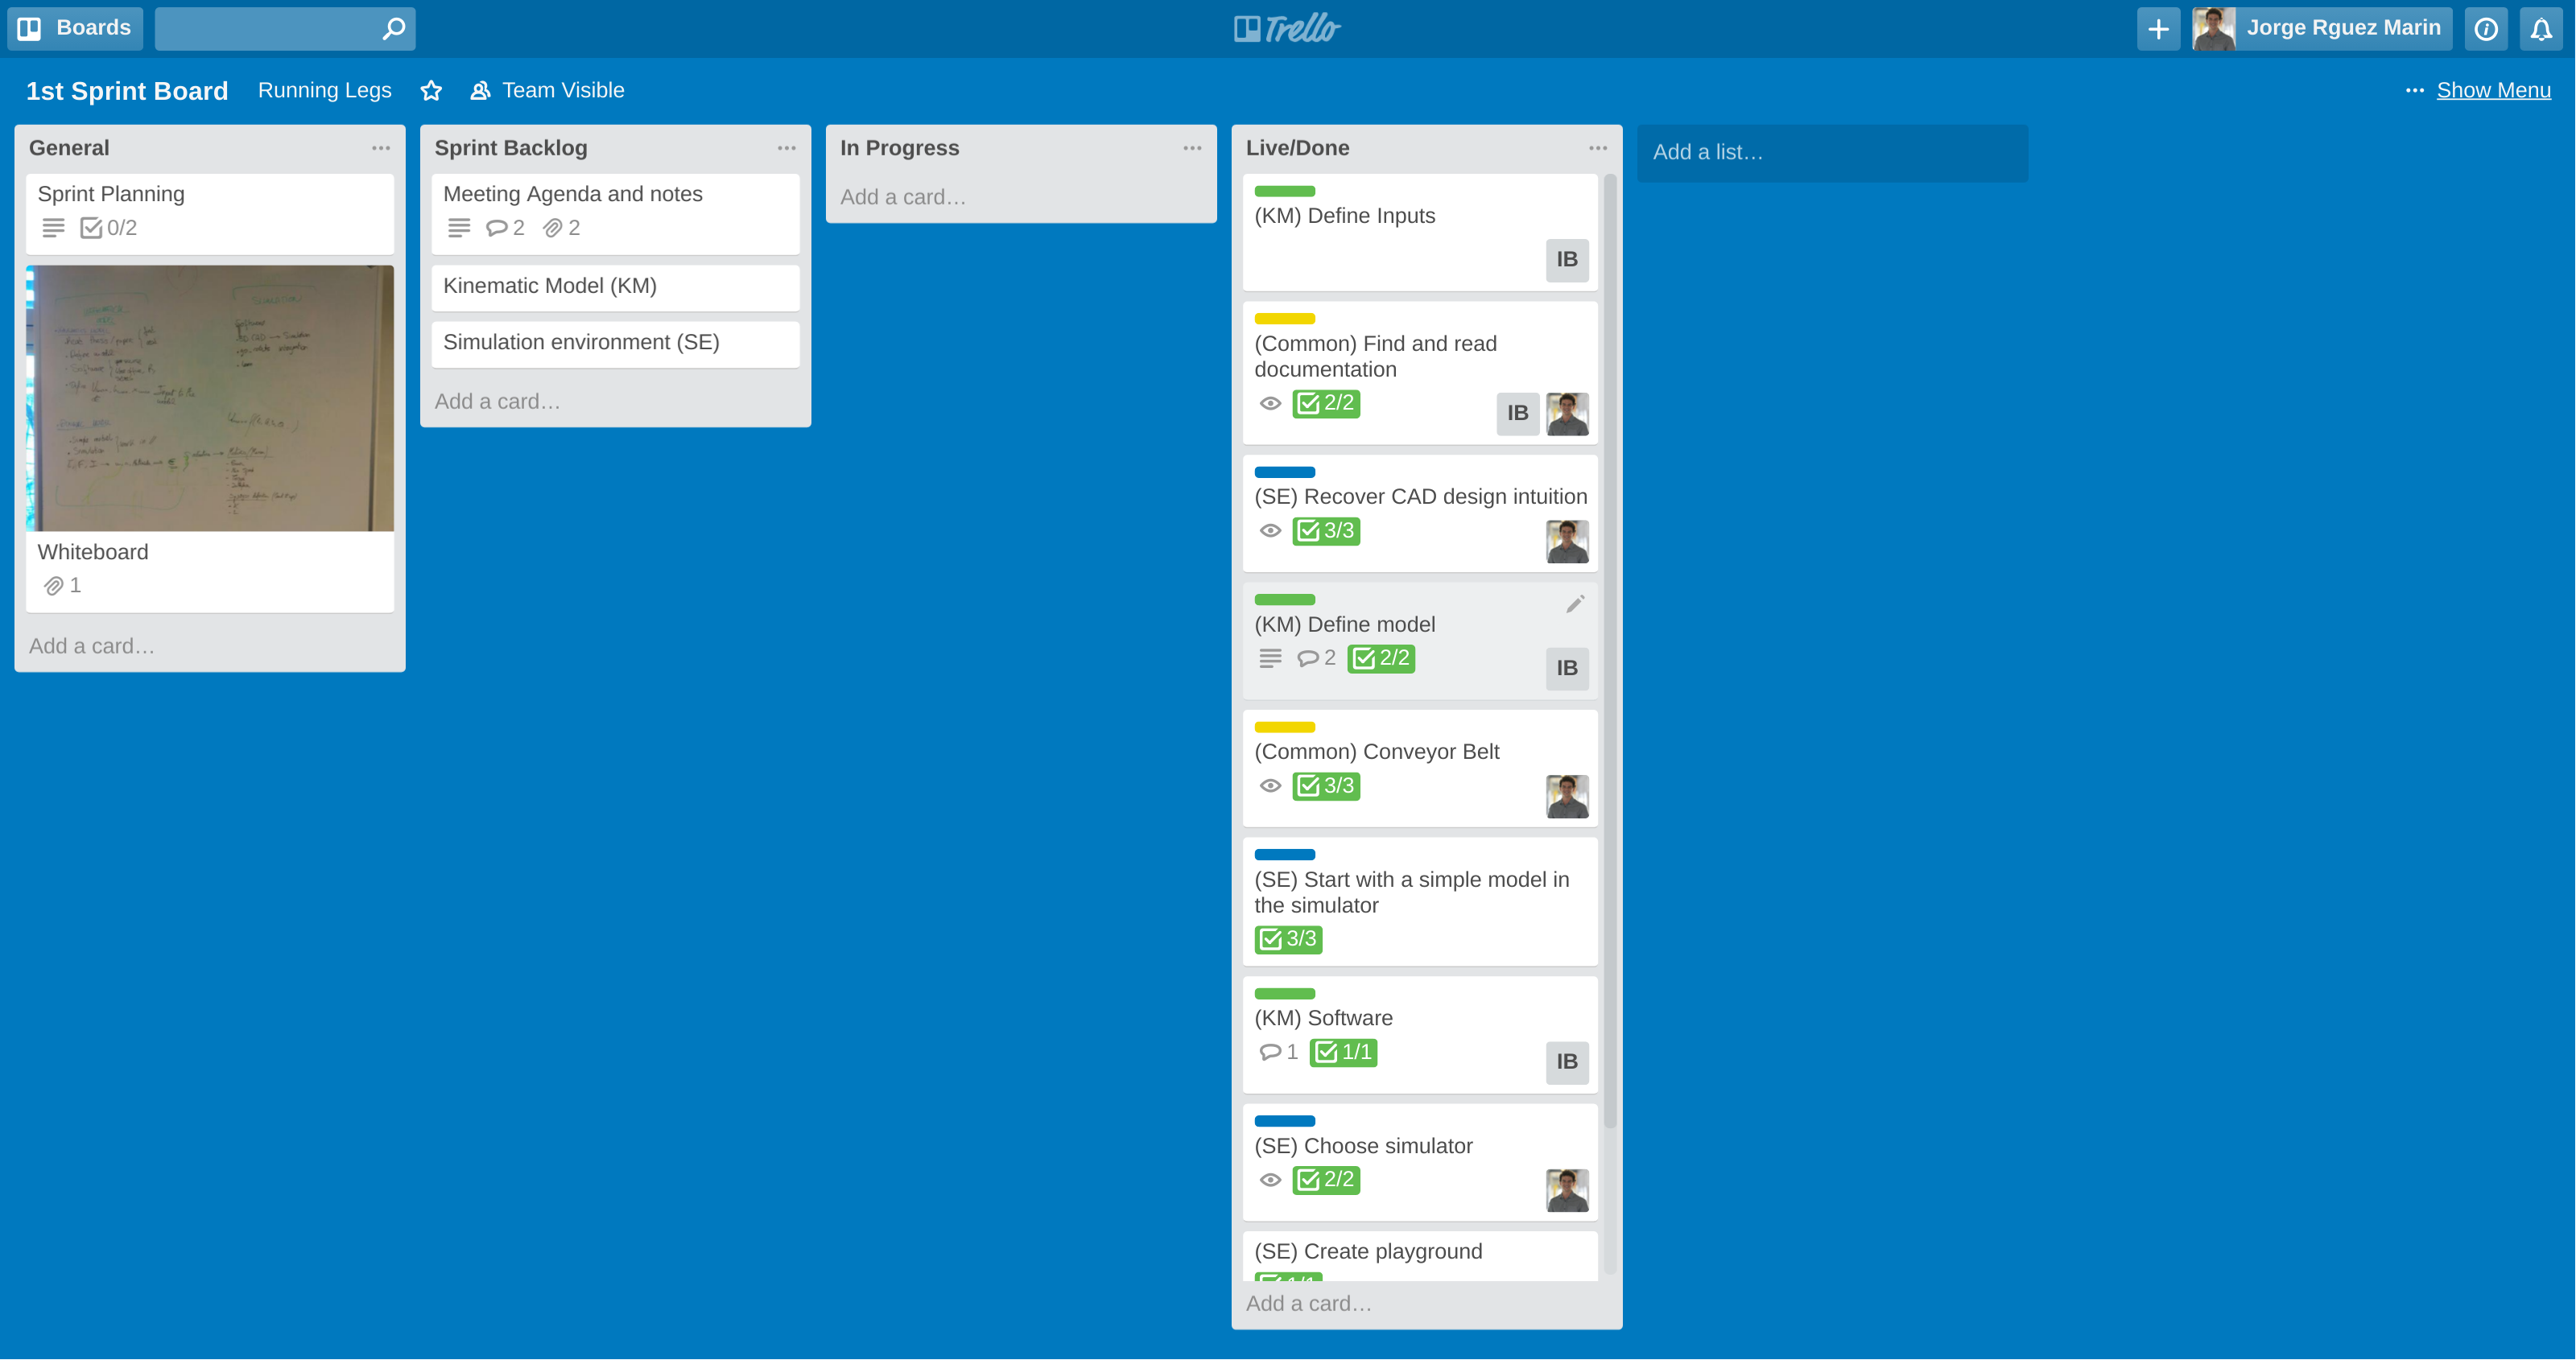
\includegraphics[width=\textwidth]{figures/trello.png}
  \caption{Screen capture of Trello showing the 1st sprint board. The three
rightmost lists are used to keep track of tasks and their state.}
  \label{fig:trello}
\end{figure}

Besides, the project has been organized in four sprints with big tasks that then are broken down into smaller jobs. The sprints are:
\begin{enumerate}
  \item \textbf{Sprint 1}
    \begin{itemize}
      \item \textbf{Goal}: Analyze robot possibilities, define the kinematic model, become familiar with the simulation environment and get ready ROS Control and software.
      \item \textbf{Duration}: 21st of January to 28th of February
      \item \textbf{Description}: An analysis of the structural possibilities of the robots is done. This is then used to start the mathematical model, which is subdivided in the kinematic and the dynamic model so the first one can be started. In parallel, all the software environment is created: from ROS control to the Gazebo structures. This will help with future extensions and will facilitate its integration for new features like the real CAD model of the robot.
    \end{itemize}
    \item \textbf{Sprint 2}
    \begin{itemize}
      \item \textbf{Goal}: Define the dynamic model, integrate Go Robots in the software structures and prepare simple simulation for testing and create example controllers.
      \item \textbf{Duration}: 3rd of March to 1st of April
      \item \textbf{Description}: The kinematic model is finished and the dynamic starts. From the software point of view, a basic simulation model is created and controlled with ROS Control. The example controllers, based on tools from Go Robots, are created and tested.
    \end{itemize}
  \item \textbf{Sprint 3}
    \begin{itemize}
      \item \textbf{Goal}: Obtain data from the mathematical model, design the CAD model of the robot and obtain the final order list.
      \item \textbf{Duration}: 2nd of April to 1st of May
      \item \textbf{Description}: The mathematical model is finished and it is used to size the motors and other components, that lets start the electro-mechanical design of the robot. If not completely finished, a list of the parts to be obtained is done and ordered.
    \end{itemize}
  \item \textbf{Sprint 4}
    \begin{itemize}
      \item \textbf{Goal}: Make electronics, print the parts with the 3D printers, receive ordered components, add software interfaces, assemble the robot, carry out tests and write thesis.
      \item \textbf{Duration}: 1st of May to 31st of May
      \item \textbf{Description}: While getting the parts, others like the 3D printed or machined parts are created. The electronic interfaces are also made. From the software perspective the interface with the real robot is implemented. The robot is assembled and the experiments carried out. Finally, the documentation of the project starts.
    \end{itemize}

\end{enumerate}

% section project_management (end)
%!TEX root = ../../../report.tex
\section{Report structure}
\label{sec:report_structure}
The present report is organized such that it starts with an overview of the evolution of legged locomotion and the current technologies applied to its study in \textbf{State of the art} [\ref{cha:state_of_the_art}].
It continues with an analysis of the robot solution and the definition of its design boundaries and criteria in the \textbf{Conception and initial analysis} chapter [\ref{cha:analysis}]
In the \textbf{Mathematical model of RuBi} [\ref{cha:mathematical_model}] a generalized kinematic and dynamic model of a biped is constructed, and the equations model of the application is sketched so that ca be used to size the actuators.
Then, in  the \textbf{Mechatronic design} chapter [\ref{cha:design}], divided into \textit{mechanics} [\ref{sec:mechanics}], \textit{Electronics} [\ref{sec:electronics}] and \textit{Software} [\ref{sec:software}], the integral and holistic design of the robot is carried out.
The \textbf{Simulation} chapter [\ref{cha:simulation}] is meant to justify the creation of the simulation tools included in the framework and explain their implementation.
It follows the \textbf{Construction process} chapter [\ref{cha:implementation}] where the processes of mechanical manufacturing, electronic wiring or the selection of the providers is explained.
In the \textbf{Experimental framework} chapter [\ref{cha:experiments}] the performed and the devised tests are presented, while in \textbf{Economical aspects} [\ref{cha:economical_aspects}] the budget analysis of the project is broken down.
The report finishes with the chapters \textbf{Results} [\ref{cha:results}], \textbf{Discussion} [\ref{cha:discussion}] and \textbf{Conclusions and further work} [\ref{cha:conclusions}].

    %!TEX root = ../../report.tex
\chapter{State of the art} % (fold)
\label{cha:state_of_the_art}
This chapter contains a concise overview of some of the major, and more relevant for this thesis, advances in artificial legged locomotion in the past 60 years.
A brief prelude of the emergence and evolution of natural, limb-based terrestrial motion and more in detail bipedalism is presented.
It is followed by a short introduction of some of the history and results from the union between the engineering field and the study of motion and legged systems. 
From the first, ancient mobile artifacts and prosthesis to the current, most advanced devices in robotics.
It continues with an exposition of three of the most pertinent breakthroughs in modern technologies that allowed to reach the current state of the art in modern autonomous walking robots.
And it finishes with a quick look to the future of the bipedal locomotion.

%!TEX root = ../../../report.tex
\section{The evolution of bipedalism}
\label{sec:bipedalism}

The current human bipedal locomotion arises from the combination of a wide variety of subsystems working in conjunction to achieve the intended gait generation according to the requirements of the situation.
The biomechanics of the limbs, consisting in bones, muscles and tendons under the control of the nervous system yields the adequate production of the different motion patterns in order to displace the body as energetically efficiently as possible.
This complex behavior is the result of 4 million years of an evolution \cite{bipedalism2} that started in primates and that has entailed both morphological and neurological changes in the human body since the first bipedal hominids to the current structure in Homo sapiens.
There exist several different theories about the reasons that originated and led to the adaption of this posture and bipedal motion.
Although different, most of them assume that most of them assume that the development of this structural and behavioral changes arose from a change in the environment in pre-hominids, for with bipedal behavior suddenly offered some kind of survival value \cite{bipedalism1}.
However, the genus Homo is not the only species that has evolved towards two-legged locomotion
Currently there are a few more species that have reached this method of displacement as a result of a natural selection process in which bipedalism offered the broadest set of advantages of the specie being the main ones listed below. 


\begin{itemize}
	\item Erect posture for a wider field of view and reach range.
	\item Free forelimbs, that could evolve towards specialized, non-locomotory applications such as object manipulation, combat, flight, etc.
	\item Faster displacement in certain species, although not generally.
\end{itemize}

Extensive research in the actuation and control structures involved in human bipedalism has been conducted from within the scientific fields of anthropology, biology, medicine, sport science and lately, several areas withing the engineering.
Its goal, as per definition of science, has been to reach a full understanding of what led to this behavior and the knowledge of how it functions, together with the discovery of ways in which it can be mimicked and improved, aiming at a more inexpensive and optimized locomotion.
This last fact has led to the belief that the next stage in the evolution of human locomotion will not come from nature as until nowadays, but from the hand of science and engineering, which has been lately depicted in literature and pop-culture as in \ref{fig:biped_evolution}.

\begin{figure}[htb]
	\centering
	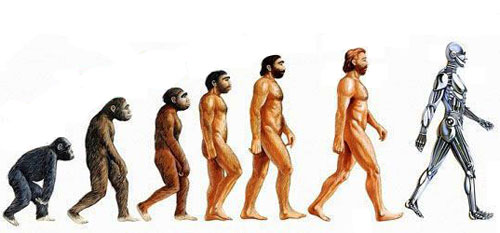
\includegraphics[width=0.8\textwidth]{figures/artificialhumans.jpg}
	\caption{Evolution of bipedalism (artistic depiction from \cite{human_evol_fig}).}
	\label{fig:biped_evolution}
\end{figure}

\subsection{Biped motion and engineering} % (fold)
\label{sub:bipedalism_and_engineering}
The discipline of engineering has been historically among the latest of the cited ones to start its contribution to the research and improvement of biped motion in a well defined manner, although its earliest contributions seem to date from ancient Egypt and India \cite{prosthetics_history}.
From the study of human bipedal motion described above, the insights emerged regarding its biomechanical and control functioning together with the need to restore, improve or imitate its capabilities led to the creation of new branches within the discipline of engineering.
The three most relevant ones for the present thesis are listed and introduced below.

\begin{enumerate}
	\item Orthotics
	\item Prosthetics
	\item Artificial legged locomotion 
\end{enumerate}

\paragraph{Orthotics} % (fold)
\label{par:orthotics}
Orthotics is a specialty within the medical field concerned with the design, manufacture and application of orthoses. An orthosis is an externally applied device used to modify the structural and functional characteristics of the neuromuscular and skeletal system, as per definition in \cite{ISO_orthosis}. 
There are orthoses dated back 2000 years ago where layers of wool were placed inside the sandals to give relief to foot fatigue or strain.
The cutting edge in this field make use of the new manufacturing technologies like 3D printing or 6 axis CNCs milling machines, which allow the creation of devices with complex shapes and novel materials.
As introduced in \cite{herbert2005preliminary}, the most critical part of the orthosis is the socket, being this the interface between the limb and the device.
Its comfortability has been improved by making use of new materials like sole-elastomers.
Sockets made of different materials can be used to get different physical properties depending on the limb of the patient, providing user adaption.
In the most advanced pole of this specialty, the powered exoskeletons can be found. Examples like \cite{zoss2006biomechanical}, \cite{veneman2007design} or \cite{pratt2004roboknee}, show how these machines are meant to help increase the phyisical capabilities of a person, handicapped or not.
% paragraph orthotics (end)

\paragraph{Prosthetics} % (fold)
\label{par:prosthetics}
Prosthetics is the field of medicine that comprises the design and creation of prosthesis, defined as artificial limbs aimed at restoring motor and sensory capabilities in amputee patients.
Since the first lower-limb prosthesis implant recorded in history, documented in the Rigveda \cite{prosthetics_history}, to the current state of the art there has been more than 3000 years of development.
This time has taken prosthetics from single-piece, non-articulated devices with no actuation or sensory feedback to the current near-natural, anthropomorphic structures and control systems adapted to the patient needs and able to closely provide the properties of a biological limb.
As in the orthoses design, the aim of the prosthetics is to mimic as closely as possible the human capabilities with designs such that they adapt to the subject as naturally as possible.
Thus, their development goes parallel to the research and understanding of the human body.
One of the most comprehensive studies in lower-limb prostheses, their design and actuation is the one provided in \cite{grimmer}.
% paragraph prosthetics (end)

\begin{figure}[htb]
	\centering
    \begin{subfigure}[b]{0.31\textwidth}
        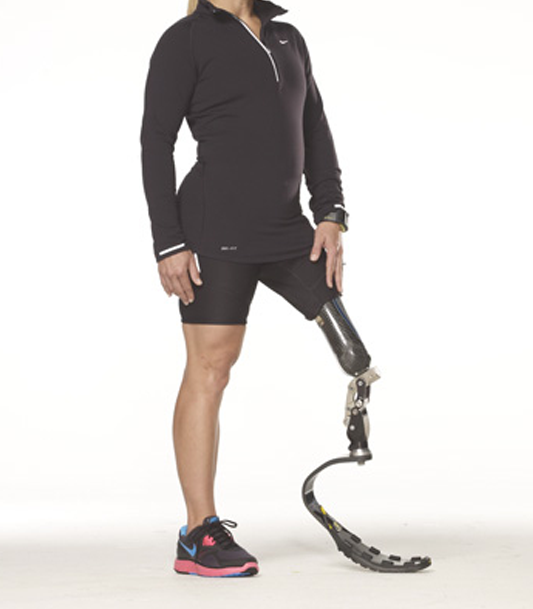
\includegraphics[width=\textwidth]{figures/prosthetic_leg.png}
        \caption{Prosthetic leg, Össur Flex-Run.}
        \label{fig:prosthetic_leg}
    \end{subfigure}
    \centering
    \begin{subfigure}[b]{0.31\textwidth}
        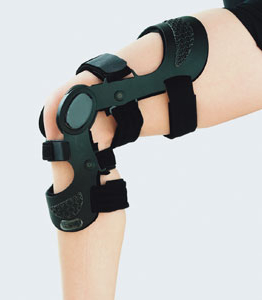
\includegraphics[width=\textwidth]{figures/orthotic_leg.jpg}
        \caption{Knee orthosis, New Hope Co.}
        \label{fig:orthotic_leg}
    \end{subfigure}s
    \centering
    \begin{subfigure}[b]{0.31\textwidth}
        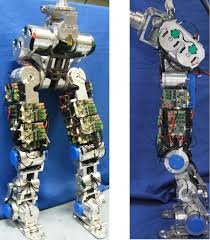
\includegraphics[width=\textwidth]{figures/robotic_leg.jpg}
        \caption{Robotic legs, COMAN robot \cite{coman}.}
        \label{fig:robotic_leg}
    \end{subfigure}
\end{figure}

\paragraph{Artificial legged locomotion} % (fold)
\label{par:humanoid_robots}  
The first artificial walking artifacts recorded date from the ancient Greece.
It is in this period when humankind first tries to imitate and replicate the structures found in nature, creating mechanisms to get a deeper knowledge of their functioning and mimic them.
But it is during the Renaissance in Europe when the developments in mechanics and the study of the nature and the human body allows to create the first automata able to walk as a predefined combination of complex mechanical operations.
It is after the Second World War, with the application of electronics and computer technology that the advancement of walking machines is revolutionized \cite{legged_mot_history1}.

The engineering branch of modern robotics has its origins in the second half of the 20th century has a conjunction of the areas of electrical and mechanical engineering and computer science.
However, its interest in achieving resemblance to the locomotion means of both humans and animals  and their capabilities arose in the 1980's.
It first crystallized into the construction of Wabot-1 at WASEDA University or the creation of the Leg Laboratory by Marc Raibert at the Massachusetts Technological Institute.
The purpose of the research in this field was the construction of useful knowledge basis on how human and animal locomotion works that could be used in the creation of legged vehicles, as described in \cite{mit_leg_lab1}.
% paragraph humanoid_robots (end)



% subsection bipedalism_and_engineering (end)


%!TEX root= ../../../report.tex

\section{From the wheel to the leg} % (fold)
\label{sec:from_the_wheel_to_the_leg}
While the wheel is a young human invention meant to facilitate terrestrial motion, legged locomotion has been the result of millions of years of adaption of the species from the aquatic to a terrestrial field.
During this time, even though other forms of motion on the ground emerged, including limbless or rolling, the tetrapod and quadrupedal motion are the ones that have proved the best performances in terrestrial displacements in terms of relative velocity or jump length, for instance.

\subsection{Discovering the wheel (in robotics)} % (fold)
\label{sub:the_wheel_in_robotics}
Despite the facts above, it was the wheel the mean chosen to implement the ability to move around on the first mobile robots such as Walter's tortoises or the John Hopkins University robot Beast \cite{first_mobile_robot}, \cite{second_mobile_robot}.
This could be explained due to the fact that, as an artificial human creation, the modeling and control of the wheel could be fully mastered during its evolution process, easing its implementation in robotic platforms.
Some examples of this are shown in Figure \ref{fig:mobile_robots}, which depicts three current applications of the wheel in robot platforms.

Although the wheel was chosen as the motion mean to face what can be considered one of the most challenging and unpredictable environment a robot can be subject to, the surface of a new planet, it was not the only option. 
The Space General Corporation firstly studied the use of multi-legged autonomous platforms for lunar exploration in the early 1960's \cite{legged_mot_history1}.
However, their use was eventually discarded due to its poor adaptability due to a too low number of DOF.
The "Spirit" robot in \ref{fig:mobile_rover}, within the NASA's Mars Exploration Rover mission, is the example of the current solution to extraplanetary exploration and a good example of the possibilities and limits entailed by wheel-based locomotion.
It was successfully launched on Mars surface in 2004 and it stayed active and operative until 2010.
However, the end of the mission came from the hand of the terrain. 
A very low-cohesion area of soil made the wheels of the device loose traction and eventually get trapped, preventing from recovering the control of the vehicle and bringing about the end of the mission.

\begin{figure}[htb]
	\centering
    \begin{subfigure}[t]{0.35\textwidth}
        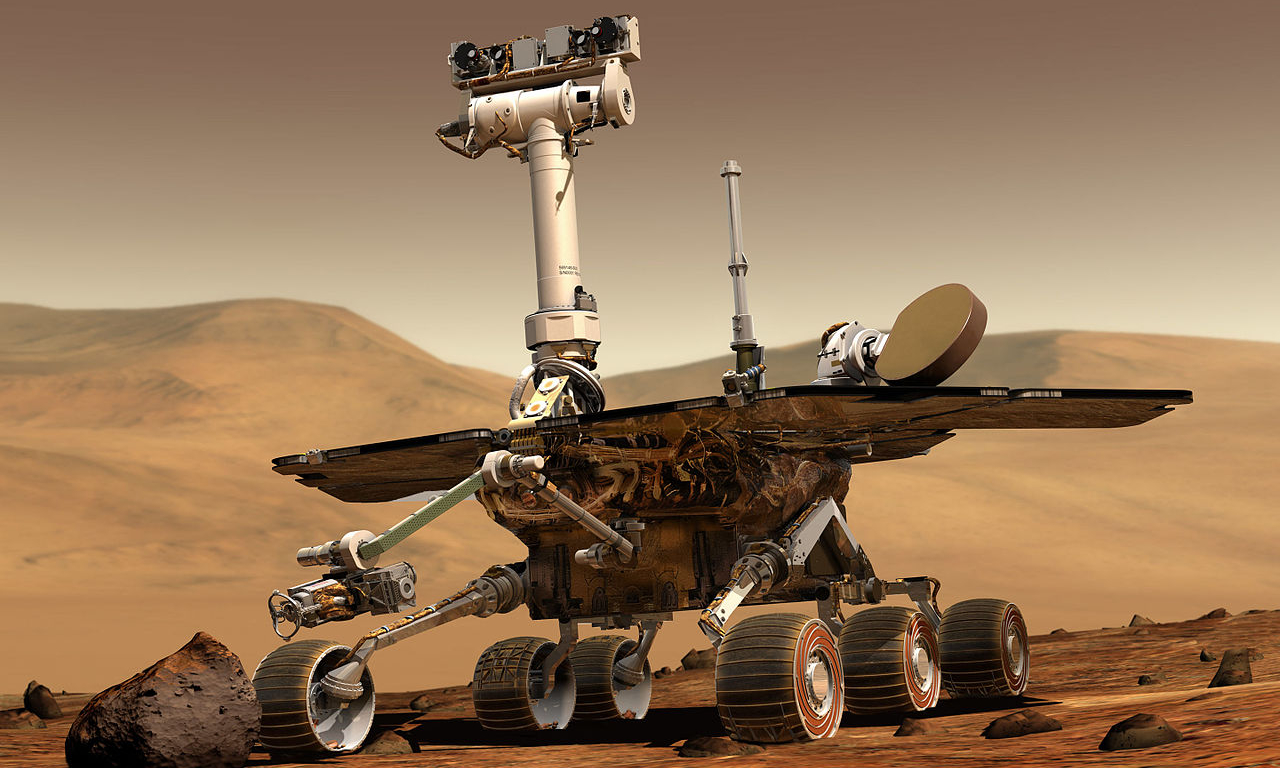
\includegraphics[width=\textwidth]{figures/mobile_rover}
        \caption{Mars Rover Spirit by NASA.}
        \label{fig:mobile_rover}
    \end{subfigure}
    \centering
    \begin{subfigure}[t]{0.35\textwidth}
        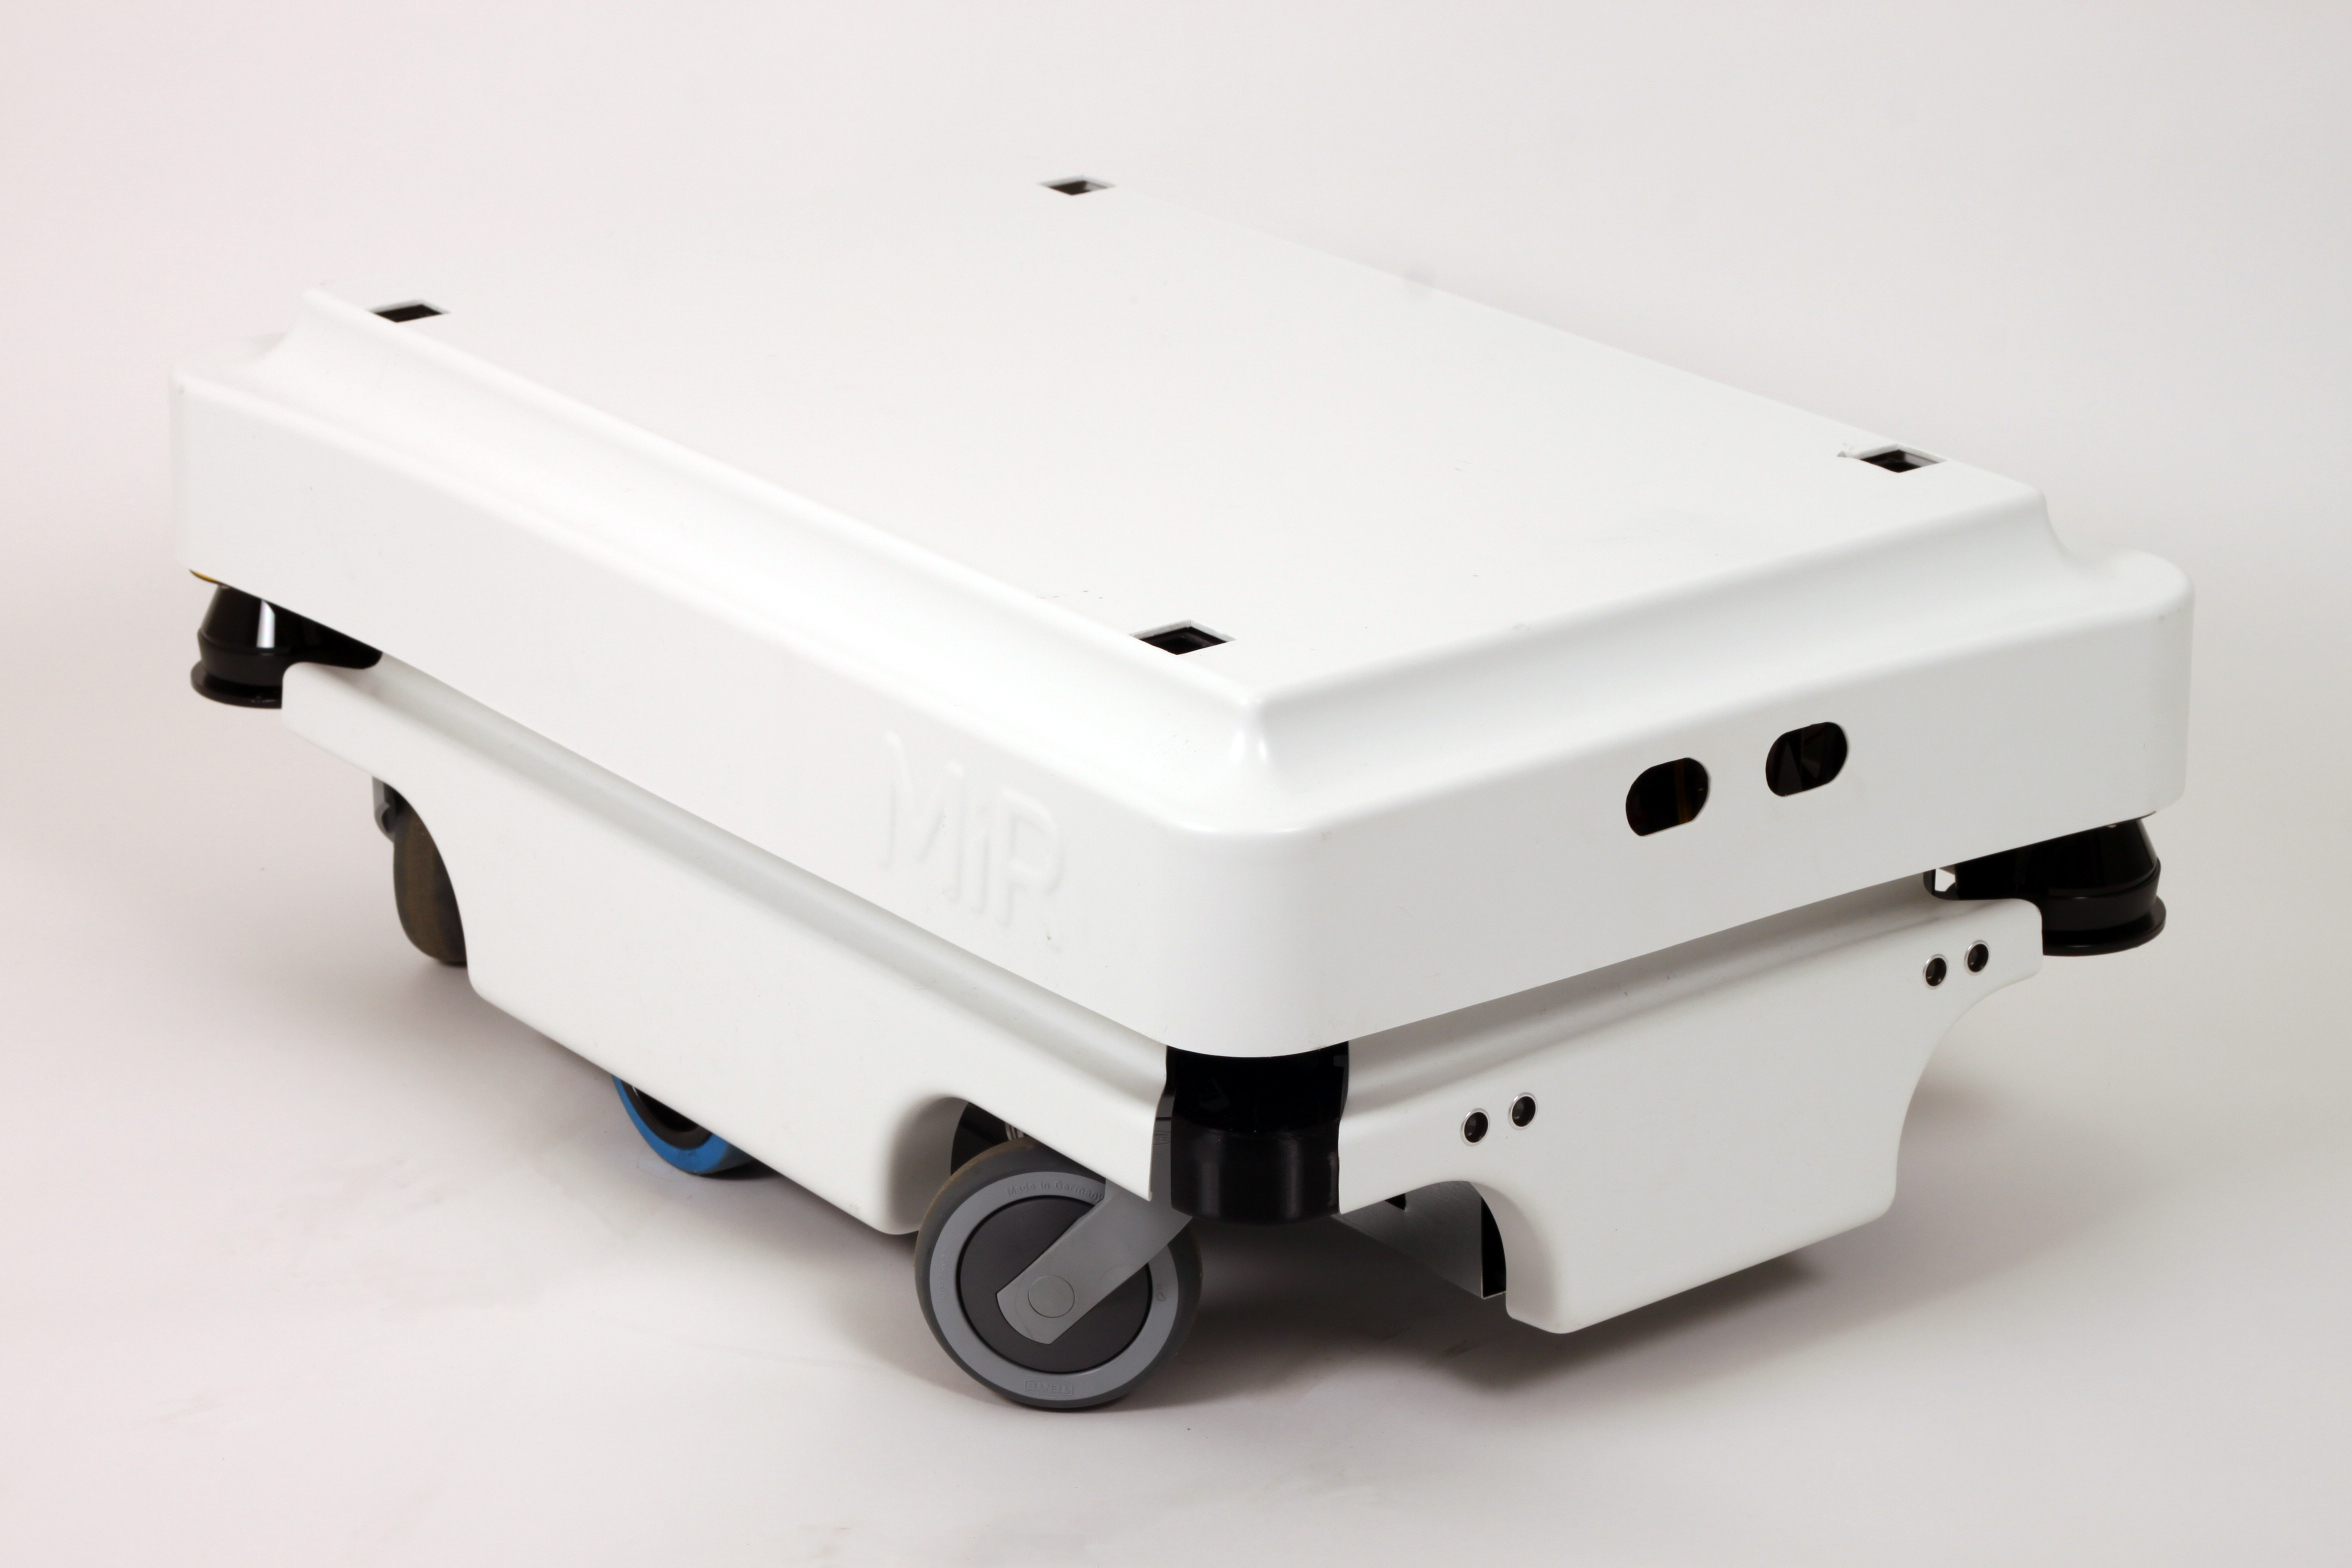
\includegraphics[width=\textwidth]{figures/mobile_mir}
        \caption{MIR 100 by MIR.}
        \label{fig:mobile_mir}
    \end{subfigure}
    \centering
    
    \begin{subfigure}[t]{0.35\textwidth}
        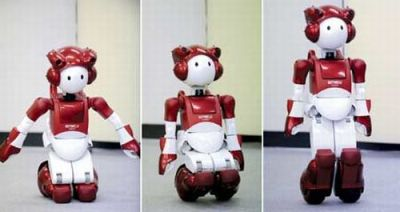
\includegraphics[width=\textwidth]{figures/mobile_hitachi}
        \caption{EMIEW2, by Hitachi.}
        \label{fig:mobile_hitachi}
    \end{subfigure}
    \caption{Examples of wheeled robot platform.}
    \label{fig:mobile_robots}
\end{figure}

Figure \ref{fig:mobile_mir} shows a MIR 100 robot, a state-of-the-art service robot designed for independent transportation and logistics in a dynamic and unpredictable environment..
As a service robot, it must fulfill strict safety standards and guarantee a secure interaction with users and other equipment while accomplishing its tasks.
Thanks to its wheels configuration, it can achieve an agile mobility, fast reaction capacity and a big load capacity.

\hfill

The EMIEW 2, in \ref{fig:mobile_hitachi}, is an example of midpoint between wheeled and legged locomotion.
Although its motion relies on steering wheels, their placement at the end of two leg-like lower-limbs provides with some of the advantages of bipedal motion, such as active suspension or impact absorption.


% subsection the_wheel_in_robotics (end)

\subsection{Achieving legged motion} % (fold)
\label{sub:legged_motion_in_robotics}
In spite of the great successes attained in the field of wheeled-robotics, possible thanks to the development in engines and the increasing computing capacity of embedded processors, mobile robots based on wheels have not been able to achieve performances in motion comparable to the ones found in nature.
Specially in uneven terrains, velocity, maneuverability, and efficiency are still problems under study.
Besides, the absence of wheels in nature as a result of darwinian evolution ultimately led to questioning \cite{dawkins} if they are truly the best mean to overcome the challenges that displacements in uneven, unknown surfaces yield for robots.
In words of Richard Dawkins \cite{dawkins} "[the wheel] is dependent for maximum efficiency on a prior invention – the road (or other smooth, hard surface)". 
Figure \ref{fig:biped_robots} contains three of the most advanced stages in legged locomotion nowadays.
They have been chosen because they are meaningful current paradigms of what brought about the revolution to the leg-based locomotion systems in the 80's: the conjunction between mechanics and control as the producers of the expected behavior \cite{mit_leg_lab1}.

The STARLeth robot in \ref{fig:starleth}, built at the Autonomous System Lab at ETH, is an example of robot legged robot inspired by nature. 
It is meant at proving that versatility, speed, robustness and efficiency can be achieved together in a legged moving platform \cite{starleth}.
But it also represents the control problems arisen from this kind of locomotion, by definition unstable and complex (12 actuated joints and 6 unactuated DOF). 

In Figure \ref{fig:kaist} the Raptor robot created at KAIST is shown.
This robot is inspired in a velociraptor structure and has been able to achieve a top stable speed on a treadmill of 46 $km/h$, making it the current fastest biped robot (although the Cheetah robot by Boston Dynamics has the record as a quadruped).
However, it is discussed here because of its simple bioinspired design, which combines prosthetic blades with a dynamic tail for stabilization and only required two motors.
This makes it a good illustration of the importance of biomechanics in the overall system.

Finally the ATLAS robot by Boston Dynamics, in \ref{fig:atlas}, represents the state of the art in bipedal autonomous platforms handling unknown, rough terrain and its interaction with dynamically changing environment.
This task for a high degree of freedom mobile manipulator as a humanoid requires a very robust interactive motion planning and control in order to quickly carry out its assignment while overcoming unpredicted situations fast and reliably enough.
The ATLAS is a good illustration of the relevance of a robust but flexible and adaptive control architecture for this kind of machines.


\begin{figure}[htb]
    \centering
    \begin{subfigure}[t]{0.40\textwidth}
        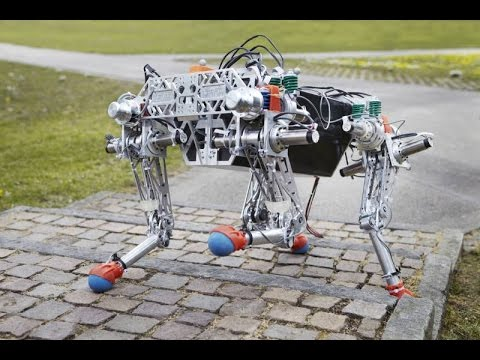
\includegraphics[width=\textwidth]{figures/starleth.jpg}
        \caption{STARLeth}
        \label{fig:starleth}
    \end{subfigure}
    \centering
    \begin{subfigure}[t]{0.40\textwidth}
        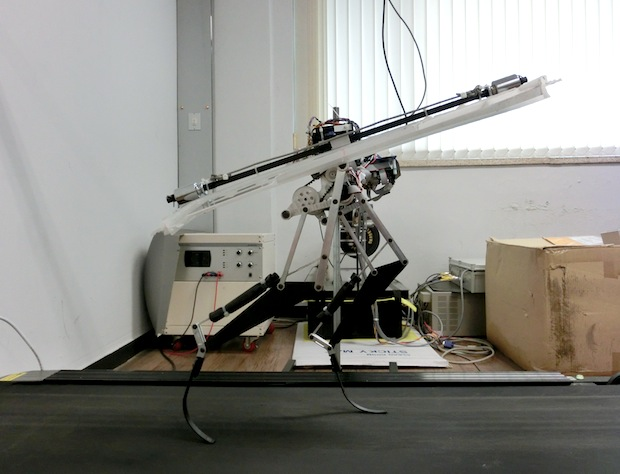
\includegraphics[width=\textwidth]{figures/biped_kaist.jpg}
        \caption{Raptor}
        \label{fig:kaist}
    \end{subfigure}
    \centering


    \begin{subfigure}[t]{0.32\textwidth}
        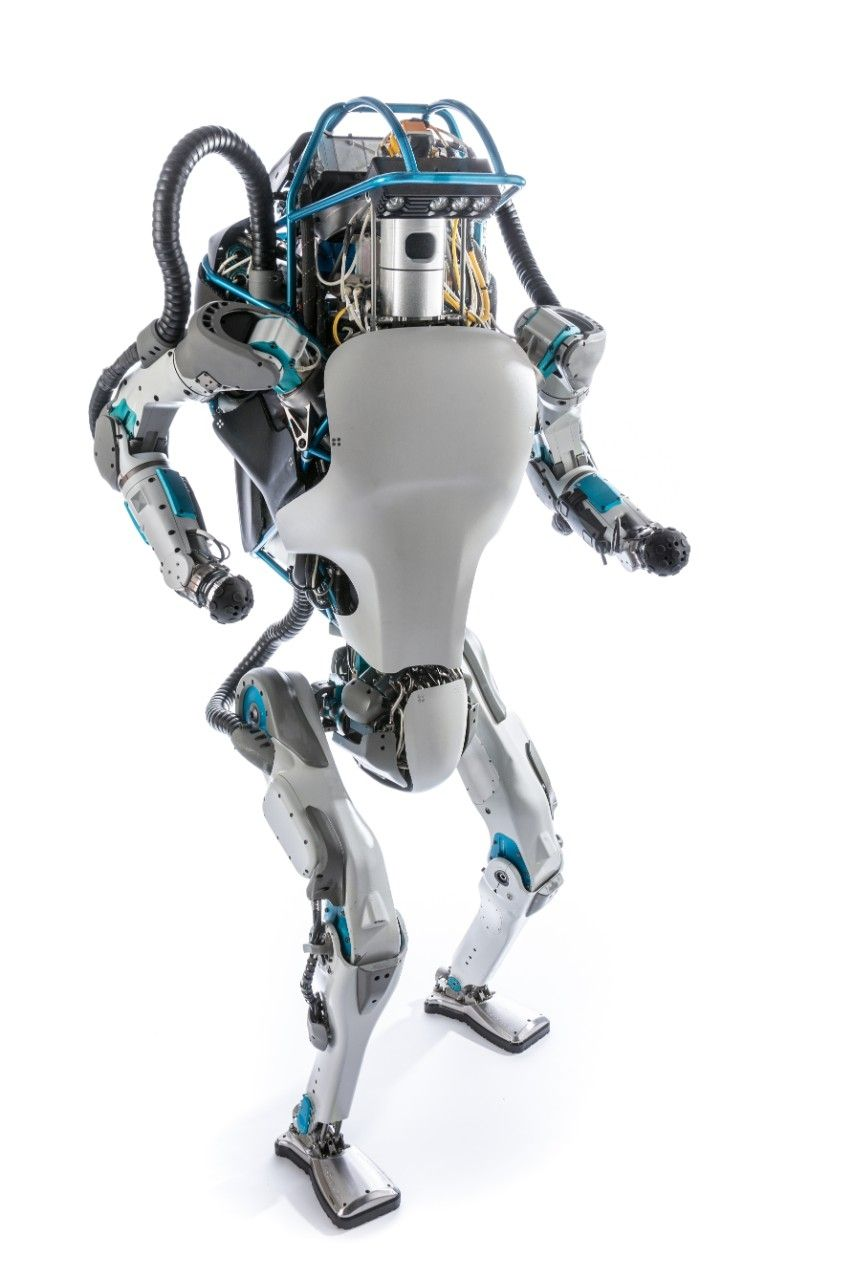
\includegraphics[width=\textwidth]{figures/biped_atlas.jpg}
        \caption{ATLAS}
        \label{fig:atlas}
    \end{subfigure}
    \caption{Examples of legged robot platforms.}
    \label{fig:biped_robots}
\end{figure}


% subsection legged_motion_in_robotics (end)





% section from_the_wheel_to_the_leg (end)
%!TEX root= ../../../report.tex

\section{Biomechanics meets Control} % (fold)
\label{sec:biomechanics_vs_control}
The first attempts to accomplish artificial walking machines in the mid-1950s were based on stiff structures and kinematic control.
There has been more than 60 years of development in several technology fields between them and the current soft, compliant and torque-controlled legged robots.
Among the main advances that gave rise to the evolution of the autonomous walking robots, three considered essential and of great relevance for this thesis are listened in \ref{list:leg_advances} and further discussed here.
Thanks to them, nowadays the research in legged robotics goes hand in hand with the study of biological locomotion systems in the attempt to imitate existing features present in nature.

\begin{itemize}
\label{list:leg_advances}
	\item The realization of the importance that a dynamic and active control has on the walking behavior, as opposed to rigid, kinematics-based motion.
	\item The conception of the embodied AI. The influence of the body in the process of thinking.
	\item The improvements in sensors/actuators performance, material science, embedded computing power and power sources.
\end{itemize}

\subsection{The relevance of body dynamics} % (fold)
\label{sub:dynamics_control}
Stiff position control for kinematic trajectory planning has lately demonstrated impressive capabilities for instance during the last DARPA learning locomotion challenge.
However, the limitations of this kind of control such as the need of a very detailed knowledge  about both the robot state vector and the environment have been also exposed.
Thus, it seems clear that the solution for robust and adaptive motion platforms has to go through the development of dynamics-based control models.
The first big steps in dynamic legged locomotion control took place in the 90's in the Leg Laboratory, at the MIT Artificial Intelligence Laboratory carried out by Marc Raibert and his team.
Their findings about the importance of active balance for stability and the possibility of creating simple and generalizable control algorithms for complex dynamic legged systems \cite{mit_leg_lab1} pushed the development of walking robots to a new stage.
Besides, they were among the pioneers in the realization of the influence of the mechanical design together with the control in the generation of complex behaviors in locomotion.
A paradigmatic example of the importance of the biomechanics and the body dynamics in the control of machines intended for locomotion is the well-known passive walker developed by McGeer \cite{passive_walking} and shown in \ref{fig:passive_walker}. 
The achievement of a human-like, efficient walking behavior without any kind control structure gave birth to the concept of morphological computation.

% subsection dynamics_control (end)
\begin{figure}[h]
	\centering
	\begin{subfigure}[b]{0.45\textwidth}
        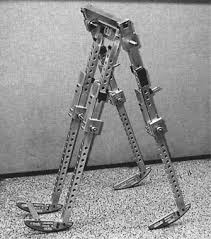
\includegraphics[width=\textwidth]{figures/passive_walker.jpg}
        \caption{McGeer's passive walker}
        \label{fig:passive_walker}
    \end{subfigure}
    \begin{subfigure}[b]{0.45\textwidth}
        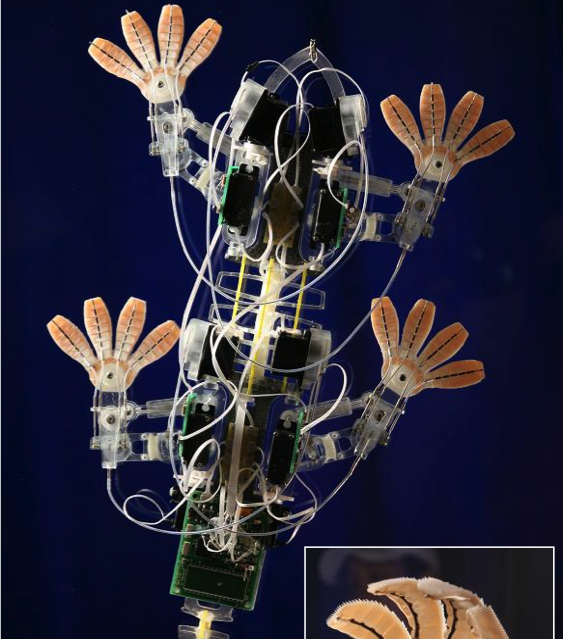
\includegraphics[width=\textwidth]{figures/Stickybot.jpg}
        \caption{Stickybot robot, Standford University}
        \label{fig:stickybot}
    \end{subfigure}
\caption{Examples of bio inspired mechanics in locomotion}
\label{fig:figure1}
\end{figure}

\subsection{Embodied AI and locomotion} % (fold)
\label{sub:the_embodiment_}
The embodiment concept came up in the Artificial Intelligence field in the 1980's as a mean to explore the influence of the body and its characteristics in the process of thinking. 
Its aim could be expressed as the search for the answer to the question, in the very convenient words of Rolf Pfeifer and Fumiya Iida, "How does walking relate to thinking?".
As introduced in \cite{pfeifer}, the original goal of AI the understanding of natural forms of intelligence that have more to do with the interaction with the real world rather than the only development of computer algorithms.

The advent of this new approach in AI caused by itself an enormous boost in the field of locomotion in robotics since it made researchers start working with mobile robots.
"The general initial conviction that locomotion and orientation were the underlying driving forces in the development of cognition, in the evolution of the brain, led to the general use of the already available wheeled robots" \cite{pfeifer}.
In the seek of an answer to the famous question "Why don’t plants have brains?", by D. Wolpert, the belief that the reason could be their incapacity for displacement led to an increasing use of mobile robots as a research tool.

Besides, the embodied AI brought about the turn to nature for inspiration in biological systems under the belief that the results of Darwinian evolution and the principle of ecological balance had created systems of greater complexity and efficiency worth studying and mimicking.
With all this, it came the understanding that complex behavior could arise from the synergistic combination of simple algorithms and the physical characteristics of the body.
Since then, mechanical compliance in the actuation, soft materials and bio inspired controllers such as CPGs for instance have been widely studied and implemented in walking machines. 
An example of this concept is the Stickybot, created in the Biomimetics and Dexterous Manipulation Lab at Standford University and shown in Figure \ref{fig:stickybot}.
% subsection the_embodiment_ (end)

\subsection{The advancement of hardware} % (fold)
\label{sub:the_advances_in_hardware}
The early timeline of the evolution in the technology utilized in biped robotic systems can be analyzed taking a look at the progression of the humanoid robots at Waseda University in Japan, in the Humanoid Research Laboratory.
In the late 1960's, Ichiro Kato and his team created the WAP-1, the first version of their first generation of humanoid robots, and the WAM-1 \ref{fig:waseda_robot1}, matching the launching of the first microprocessors.
The WAP-1 robot was moved by very slow pneumatic artificial muscles, first developed in the 1950's but not widely commercialized until the beginning of the 80's, and had to be connected to a large external computer frame for its control. 
Later version WAP-2 and WAP-3 incorporated controller-based memory and PWM-driven actuators, created at the end of the 1960's, that allowed to reach three-dimensional walking at near human-like locomotion speeds for the first time in history.
Kato also created the first full-size humanoid robot, the Wabot-I, and since the beginning of the 80's his group and him applied for the first time 16-bit microcomputers (introduced in 1973) to the implementation of quasy-dynamic walking control \cite{biped_robots_history}.
On of the latest achievements of Kato Laboratory is the WABIAN-2R, in \ref{fig:waseda_robot2}.

\begin{figure}[h]
	\centering
    \begin{subfigure}[b]{0.4\textwidth}
        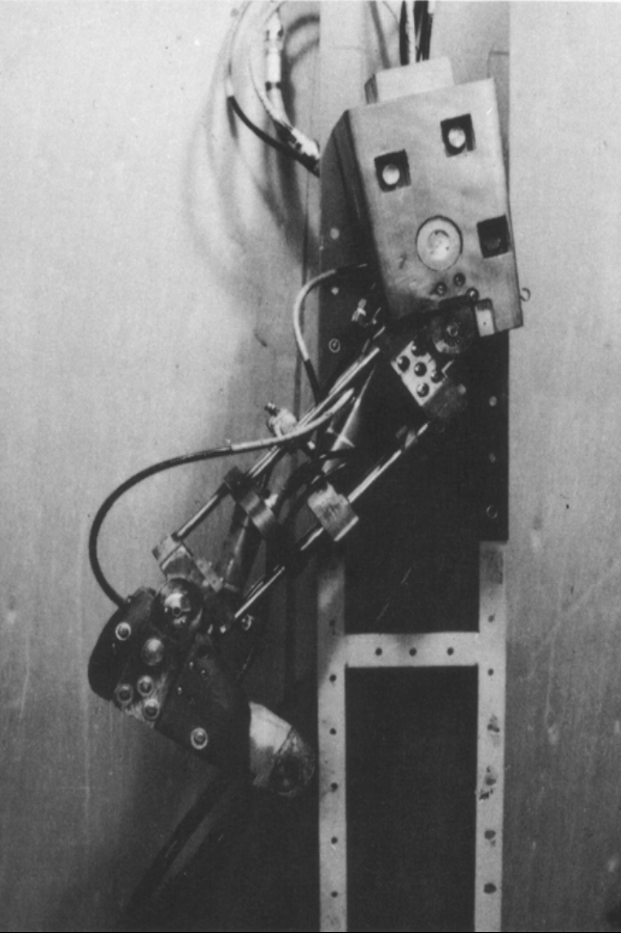
\includegraphics[width=\textwidth]{figures/waseda1.pdf}
        \caption{WAM-1 (1966)}
        \label{fig:waseda_robot1}
    \end{subfigure}
    \centering
    \begin{subfigure}[b]{0.4\textwidth}
        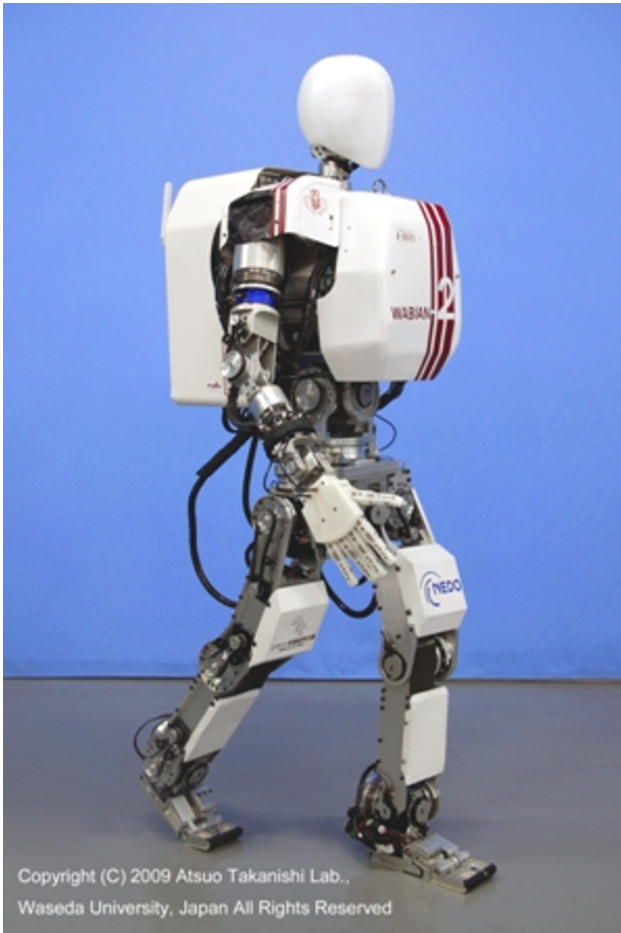
\includegraphics[width=\textwidth]{figures/waseda2.pdf}
        \caption{WABIAN-2R (2006)}
        \label{fig:waseda_robot2}
    \end{subfigure}
\end{figure}

The above is just an example of how during the last two decades of the 20th century and the beginning of the 21st, the progresses in sensing, actuation and control has largely influenced the development of legged locomotion in robotics.
However, despite the latest and impressive enhancements in mechatronics, its evolution continues presenting challenges for the advancement of autonomous biped robots.
Nowadays, the main requirements from a hardware point of view are listed in \ref{list:hardware_challenges} as per \cite{biped_robots_history}.

\begin{itemize}
	\item Energy-efficient and high-performance actuators with high torque-to-weight ratio and high torque-to-volume ratio.
	\item Highly reliable while economical sensors.
	\item Lightweight but mechanically strong materials for construction of the structure and mechanism.
	\item Fast, high computing power, and economical dedicated computer system robust against hostile situations of nature.
	\item Lighter power sources with greater autonomy.
\label{list:hardware_challenges}
\end{itemize}

In spite of this, it seems that the progress in legged autonomous systems will come from the hand of the introduction in the robotics field of recent areas in science as nanotechnology or smart materials.
Together with this, the new findings in microelectronics and the miniaturization of computers and batteries will help overcome the current challenges.


% subsection the_advances_in_hardware (end)


% section biomechanics_vs_control (end)
%!TEX root= ../../../report.tex

\section{The next generation of bipeds} % (fold)
\label{sec:the_next_generation_of_bipeds}
It appears clear now that the evolution of bipedal locomotion has in the last decades suffered a wide-reaching change in its conditions with the entrance on the stage of robotics science and its research in walking machines.
It still stands difficult, however, to foresee the paths that the advancements in artificial bipedalism will take without the risk of getting lost in speculations.
Notwithstanding, the latest breakthroughs yield reasons to believe that the next generation of walking machines will resemble more and more the physiological designs developed by nature, although only to the extent that the state-of-the-art mechantronics allows.
This last fact entails that a complete imitation of living biological structures is yet out of the reach of engineering, thus making its goal not to just copy, but to understand the underlying principles that drive biology and transfer them to the new synthetic creations with the existing technology.



However, the latest advances in some of the youngest areas of the engineering seem to be close to bring about a change in the so far unaltered rules of the game.
The progresses in AI and in the design of genetic algorithms have arisen the possibility of not only striving for mimicking nature, but also replicating its fundamental processes, artificially accelerating and modifying them.
In the next decades, nature could stop being the only motor of evolution and from there, the possibilities are boundless.

% section the_next_generation_of_bipeds (end)
%%!TEX root = ../../report.tex
\chapter{State of the art} % (fold)
\label{cha:state_of_the_art}
This chapter contains a concise overview of some of the major, and more relevant for this thesis, advances in artificial legged locomotion in the past 60 years.
A brief prelude of the emergence and evolution of natural, limb-based terrestrial motion and more in detail bipedalism is presented.
It is followed by a short introduction of some of the history and results from the union between the engineering field and the study of motion and legged systems. 
From the first, ancient mobile artifacts and prosthesis to the current, most advanced devices in robotics.
It continues with an exposition of three of the most pertinent breakthroughs in modern technologies that allowed to reach the current state of the art in modern autonomous walking robots.
And it finishes with a quick look to the future of the bipedal locomotion.

%!TEX root = ../../../report.tex
\section{The evolution of bipedalism}
\label{sec:bipedalism}

The current human bipedal locomotion arises from the combination of a wide variety of subsystems working in conjunction to achieve the intended gait generation according to the requirements of the situation.
The biomechanics of the limbs, consisting in bones, muscles and tendons under the control of the nervous system yields the adequate production of the different motion patterns in order to displace the body as energetically efficiently as possible.
This complex behavior is the result of 4 million years of an evolution \cite{bipedalism2} that started in primates and that has entailed both morphological and neurological changes in the human body since the first bipedal hominids to the current structure in Homo sapiens.
There exist several different theories about the reasons that originated and led to the adaption of this posture and bipedal motion.
Although different, most of them assume that most of them assume that the development of this structural and behavioral changes arose from a change in the environment in pre-hominids, for with bipedal behavior suddenly offered some kind of survival value \cite{bipedalism1}.
However, the genus Homo is not the only species that has evolved towards two-legged locomotion
Currently there are a few more species that have reached this method of displacement as a result of a natural selection process in which bipedalism offered the broadest set of advantages of the specie being the main ones listed below. 


\begin{itemize}
	\item Erect posture for a wider field of view and reach range.
	\item Free forelimbs, that could evolve towards specialized, non-locomotory applications such as object manipulation, combat, flight, etc.
	\item Faster displacement in certain species, although not generally.
\end{itemize}

Extensive research in the actuation and control structures involved in human bipedalism has been conducted from within the scientific fields of anthropology, biology, medicine, sport science and lately, several areas withing the engineering.
Its goal, as per definition of science, has been to reach a full understanding of what led to this behavior and the knowledge of how it functions, together with the discovery of ways in which it can be mimicked and improved, aiming at a more inexpensive and optimized locomotion.
This last fact has led to the belief that the next stage in the evolution of human locomotion will not come from nature as until nowadays, but from the hand of science and engineering, which has been lately depicted in literature and pop-culture as in \ref{fig:biped_evolution}.

\begin{figure}[htb]
	\centering
	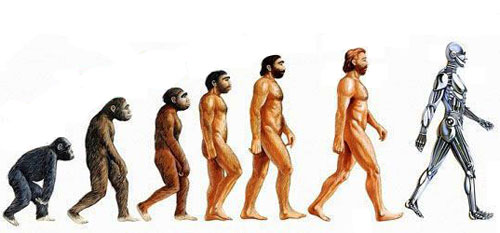
\includegraphics[width=0.8\textwidth]{figures/artificialhumans.jpg}
	\caption{Evolution of bipedalism (artistic depiction from \cite{human_evol_fig}).}
	\label{fig:biped_evolution}
\end{figure}

\subsection{Biped motion and engineering} % (fold)
\label{sub:bipedalism_and_engineering}
The discipline of engineering has been historically among the latest of the cited ones to start its contribution to the research and improvement of biped motion in a well defined manner, although its earliest contributions seem to date from ancient Egypt and India \cite{prosthetics_history}.
From the study of human bipedal motion described above, the insights emerged regarding its biomechanical and control functioning together with the need to restore, improve or imitate its capabilities led to the creation of new branches within the discipline of engineering.
The three most relevant ones for the present thesis are listed and introduced below.

\begin{enumerate}
	\item Orthotics
	\item Prosthetics
	\item Artificial legged locomotion 
\end{enumerate}

\paragraph{Orthotics} % (fold)
\label{par:orthotics}
Orthotics is a specialty within the medical field concerned with the design, manufacture and application of orthoses. An orthosis is an externally applied device used to modify the structural and functional characteristics of the neuromuscular and skeletal system, as per definition in \cite{ISO_orthosis}. 
There are orthoses dated back 2000 years ago where layers of wool were placed inside the sandals to give relief to foot fatigue or strain.
The cutting edge in this field make use of the new manufacturing technologies like 3D printing or 6 axis CNCs milling machines, which allow the creation of devices with complex shapes and novel materials.
As introduced in \cite{herbert2005preliminary}, the most critical part of the orthosis is the socket, being this the interface between the limb and the device.
Its comfortability has been improved by making use of new materials like sole-elastomers.
Sockets made of different materials can be used to get different physical properties depending on the limb of the patient, providing user adaption.
In the most advanced pole of this specialty, the powered exoskeletons can be found. Examples like \cite{zoss2006biomechanical}, \cite{veneman2007design} or \cite{pratt2004roboknee}, show how these machines are meant to help increase the phyisical capabilities of a person, handicapped or not.
% paragraph orthotics (end)

\paragraph{Prosthetics} % (fold)
\label{par:prosthetics}
Prosthetics is the field of medicine that comprises the design and creation of prosthesis, defined as artificial limbs aimed at restoring motor and sensory capabilities in amputee patients.
Since the first lower-limb prosthesis implant recorded in history, documented in the Rigveda \cite{prosthetics_history}, to the current state of the art there has been more than 3000 years of development.
This time has taken prosthetics from single-piece, non-articulated devices with no actuation or sensory feedback to the current near-natural, anthropomorphic structures and control systems adapted to the patient needs and able to closely provide the properties of a biological limb.
As in the orthoses design, the aim of the prosthetics is to mimic as closely as possible the human capabilities with designs such that they adapt to the subject as naturally as possible.
Thus, their development goes parallel to the research and understanding of the human body.
One of the most comprehensive studies in lower-limb prostheses, their design and actuation is the one provided in \cite{grimmer}.
% paragraph prosthetics (end)

\begin{figure}[htb]
	\centering
    \begin{subfigure}[b]{0.31\textwidth}
        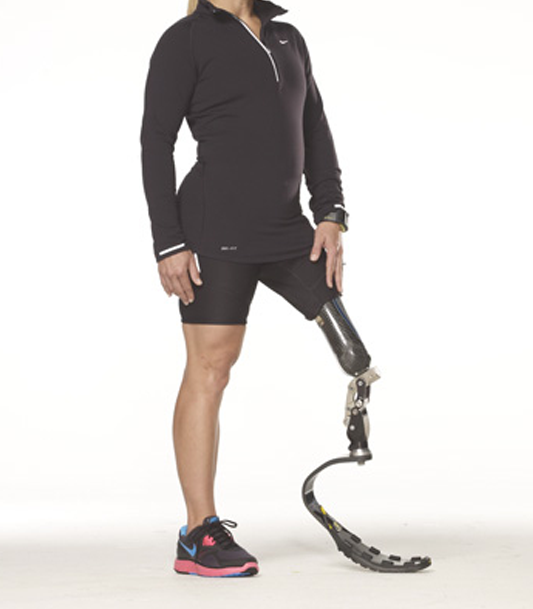
\includegraphics[width=\textwidth]{figures/prosthetic_leg.png}
        \caption{Prosthetic leg, Össur Flex-Run.}
        \label{fig:prosthetic_leg}
    \end{subfigure}
    \centering
    \begin{subfigure}[b]{0.31\textwidth}
        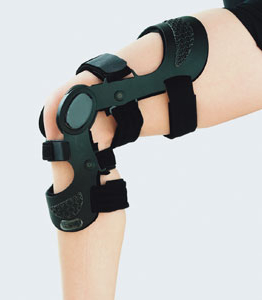
\includegraphics[width=\textwidth]{figures/orthotic_leg.jpg}
        \caption{Knee orthosis, New Hope Co.}
        \label{fig:orthotic_leg}
    \end{subfigure}s
    \centering
    \begin{subfigure}[b]{0.31\textwidth}
        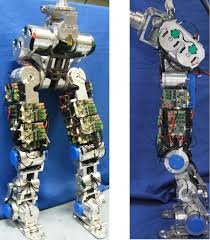
\includegraphics[width=\textwidth]{figures/robotic_leg.jpg}
        \caption{Robotic legs, COMAN robot \cite{coman}.}
        \label{fig:robotic_leg}
    \end{subfigure}
\end{figure}

\paragraph{Artificial legged locomotion} % (fold)
\label{par:humanoid_robots}  
The first artificial walking artifacts recorded date from the ancient Greece.
It is in this period when humankind first tries to imitate and replicate the structures found in nature, creating mechanisms to get a deeper knowledge of their functioning and mimic them.
But it is during the Renaissance in Europe when the developments in mechanics and the study of the nature and the human body allows to create the first automata able to walk as a predefined combination of complex mechanical operations.
It is after the Second World War, with the application of electronics and computer technology that the advancement of walking machines is revolutionized \cite{legged_mot_history1}.

The engineering branch of modern robotics has its origins in the second half of the 20th century has a conjunction of the areas of electrical and mechanical engineering and computer science.
However, its interest in achieving resemblance to the locomotion means of both humans and animals  and their capabilities arose in the 1980's.
It first crystallized into the construction of Wabot-1 at WASEDA University or the creation of the Leg Laboratory by Marc Raibert at the Massachusetts Technological Institute.
The purpose of the research in this field was the construction of useful knowledge basis on how human and animal locomotion works that could be used in the creation of legged vehicles, as described in \cite{mit_leg_lab1}.
% paragraph humanoid_robots (end)



% subsection bipedalism_and_engineering (end)


%!TEX root= ../../../report.tex

\section{From the wheel to the leg} % (fold)
\label{sec:from_the_wheel_to_the_leg}
While the wheel is a young human invention meant to facilitate terrestrial motion, legged locomotion has been the result of millions of years of adaption of the species from the aquatic to a terrestrial field.
During this time, even though other forms of motion on the ground emerged, including limbless or rolling, the tetrapod and quadrupedal motion are the ones that have proved the best performances in terrestrial displacements in terms of relative velocity or jump length, for instance.

\subsection{Discovering the wheel (in robotics)} % (fold)
\label{sub:the_wheel_in_robotics}
Despite the facts above, it was the wheel the mean chosen to implement the ability to move around on the first mobile robots such as Walter's tortoises or the John Hopkins University robot Beast \cite{first_mobile_robot}, \cite{second_mobile_robot}.
This could be explained due to the fact that, as an artificial human creation, the modeling and control of the wheel could be fully mastered during its evolution process, easing its implementation in robotic platforms.
Some examples of this are shown in Figure \ref{fig:mobile_robots}, which depicts three current applications of the wheel in robot platforms.

Although the wheel was chosen as the motion mean to face what can be considered one of the most challenging and unpredictable environment a robot can be subject to, the surface of a new planet, it was not the only option. 
The Space General Corporation firstly studied the use of multi-legged autonomous platforms for lunar exploration in the early 1960's \cite{legged_mot_history1}.
However, their use was eventually discarded due to its poor adaptability due to a too low number of DOF.
The "Spirit" robot in \ref{fig:mobile_rover}, within the NASA's Mars Exploration Rover mission, is the example of the current solution to extraplanetary exploration and a good example of the possibilities and limits entailed by wheel-based locomotion.
It was successfully launched on Mars surface in 2004 and it stayed active and operative until 2010.
However, the end of the mission came from the hand of the terrain. 
A very low-cohesion area of soil made the wheels of the device loose traction and eventually get trapped, preventing from recovering the control of the vehicle and bringing about the end of the mission.

\begin{figure}[htb]
	\centering
    \begin{subfigure}[t]{0.35\textwidth}
        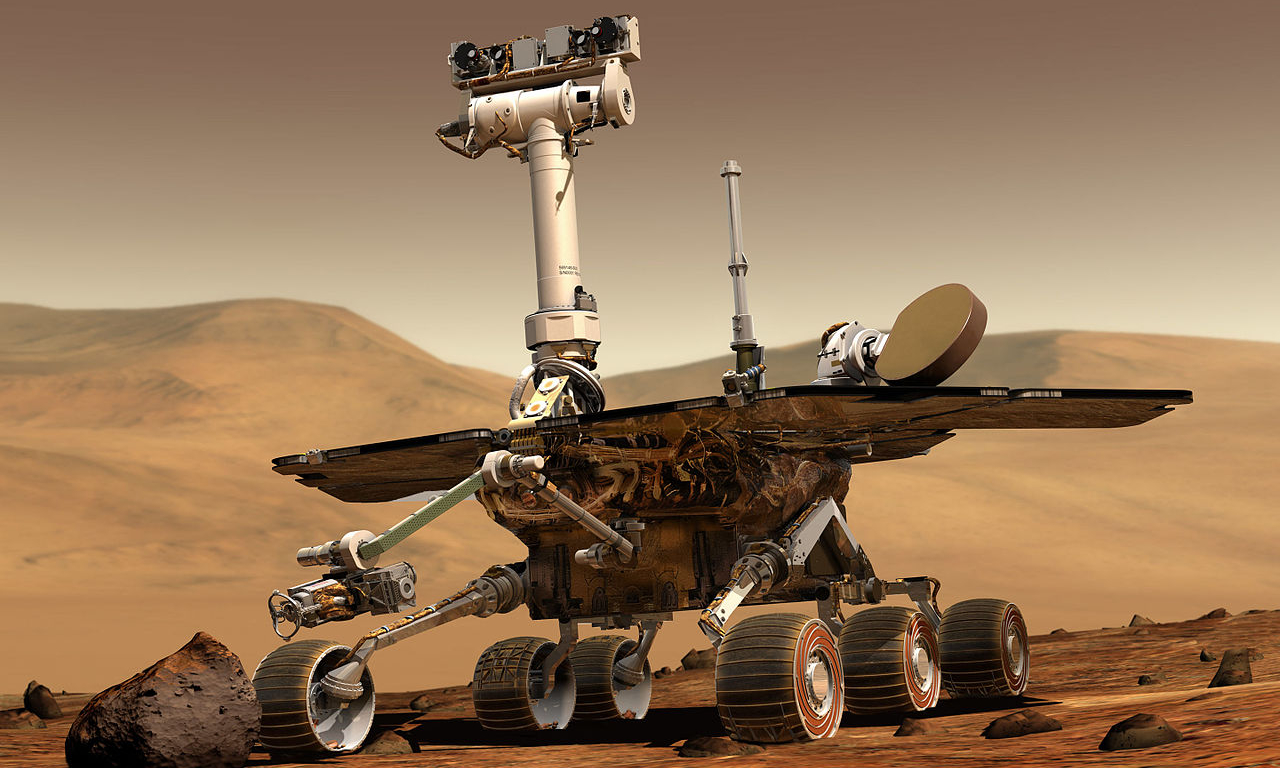
\includegraphics[width=\textwidth]{figures/mobile_rover}
        \caption{Mars Rover Spirit by NASA.}
        \label{fig:mobile_rover}
    \end{subfigure}
    \centering
    \begin{subfigure}[t]{0.35\textwidth}
        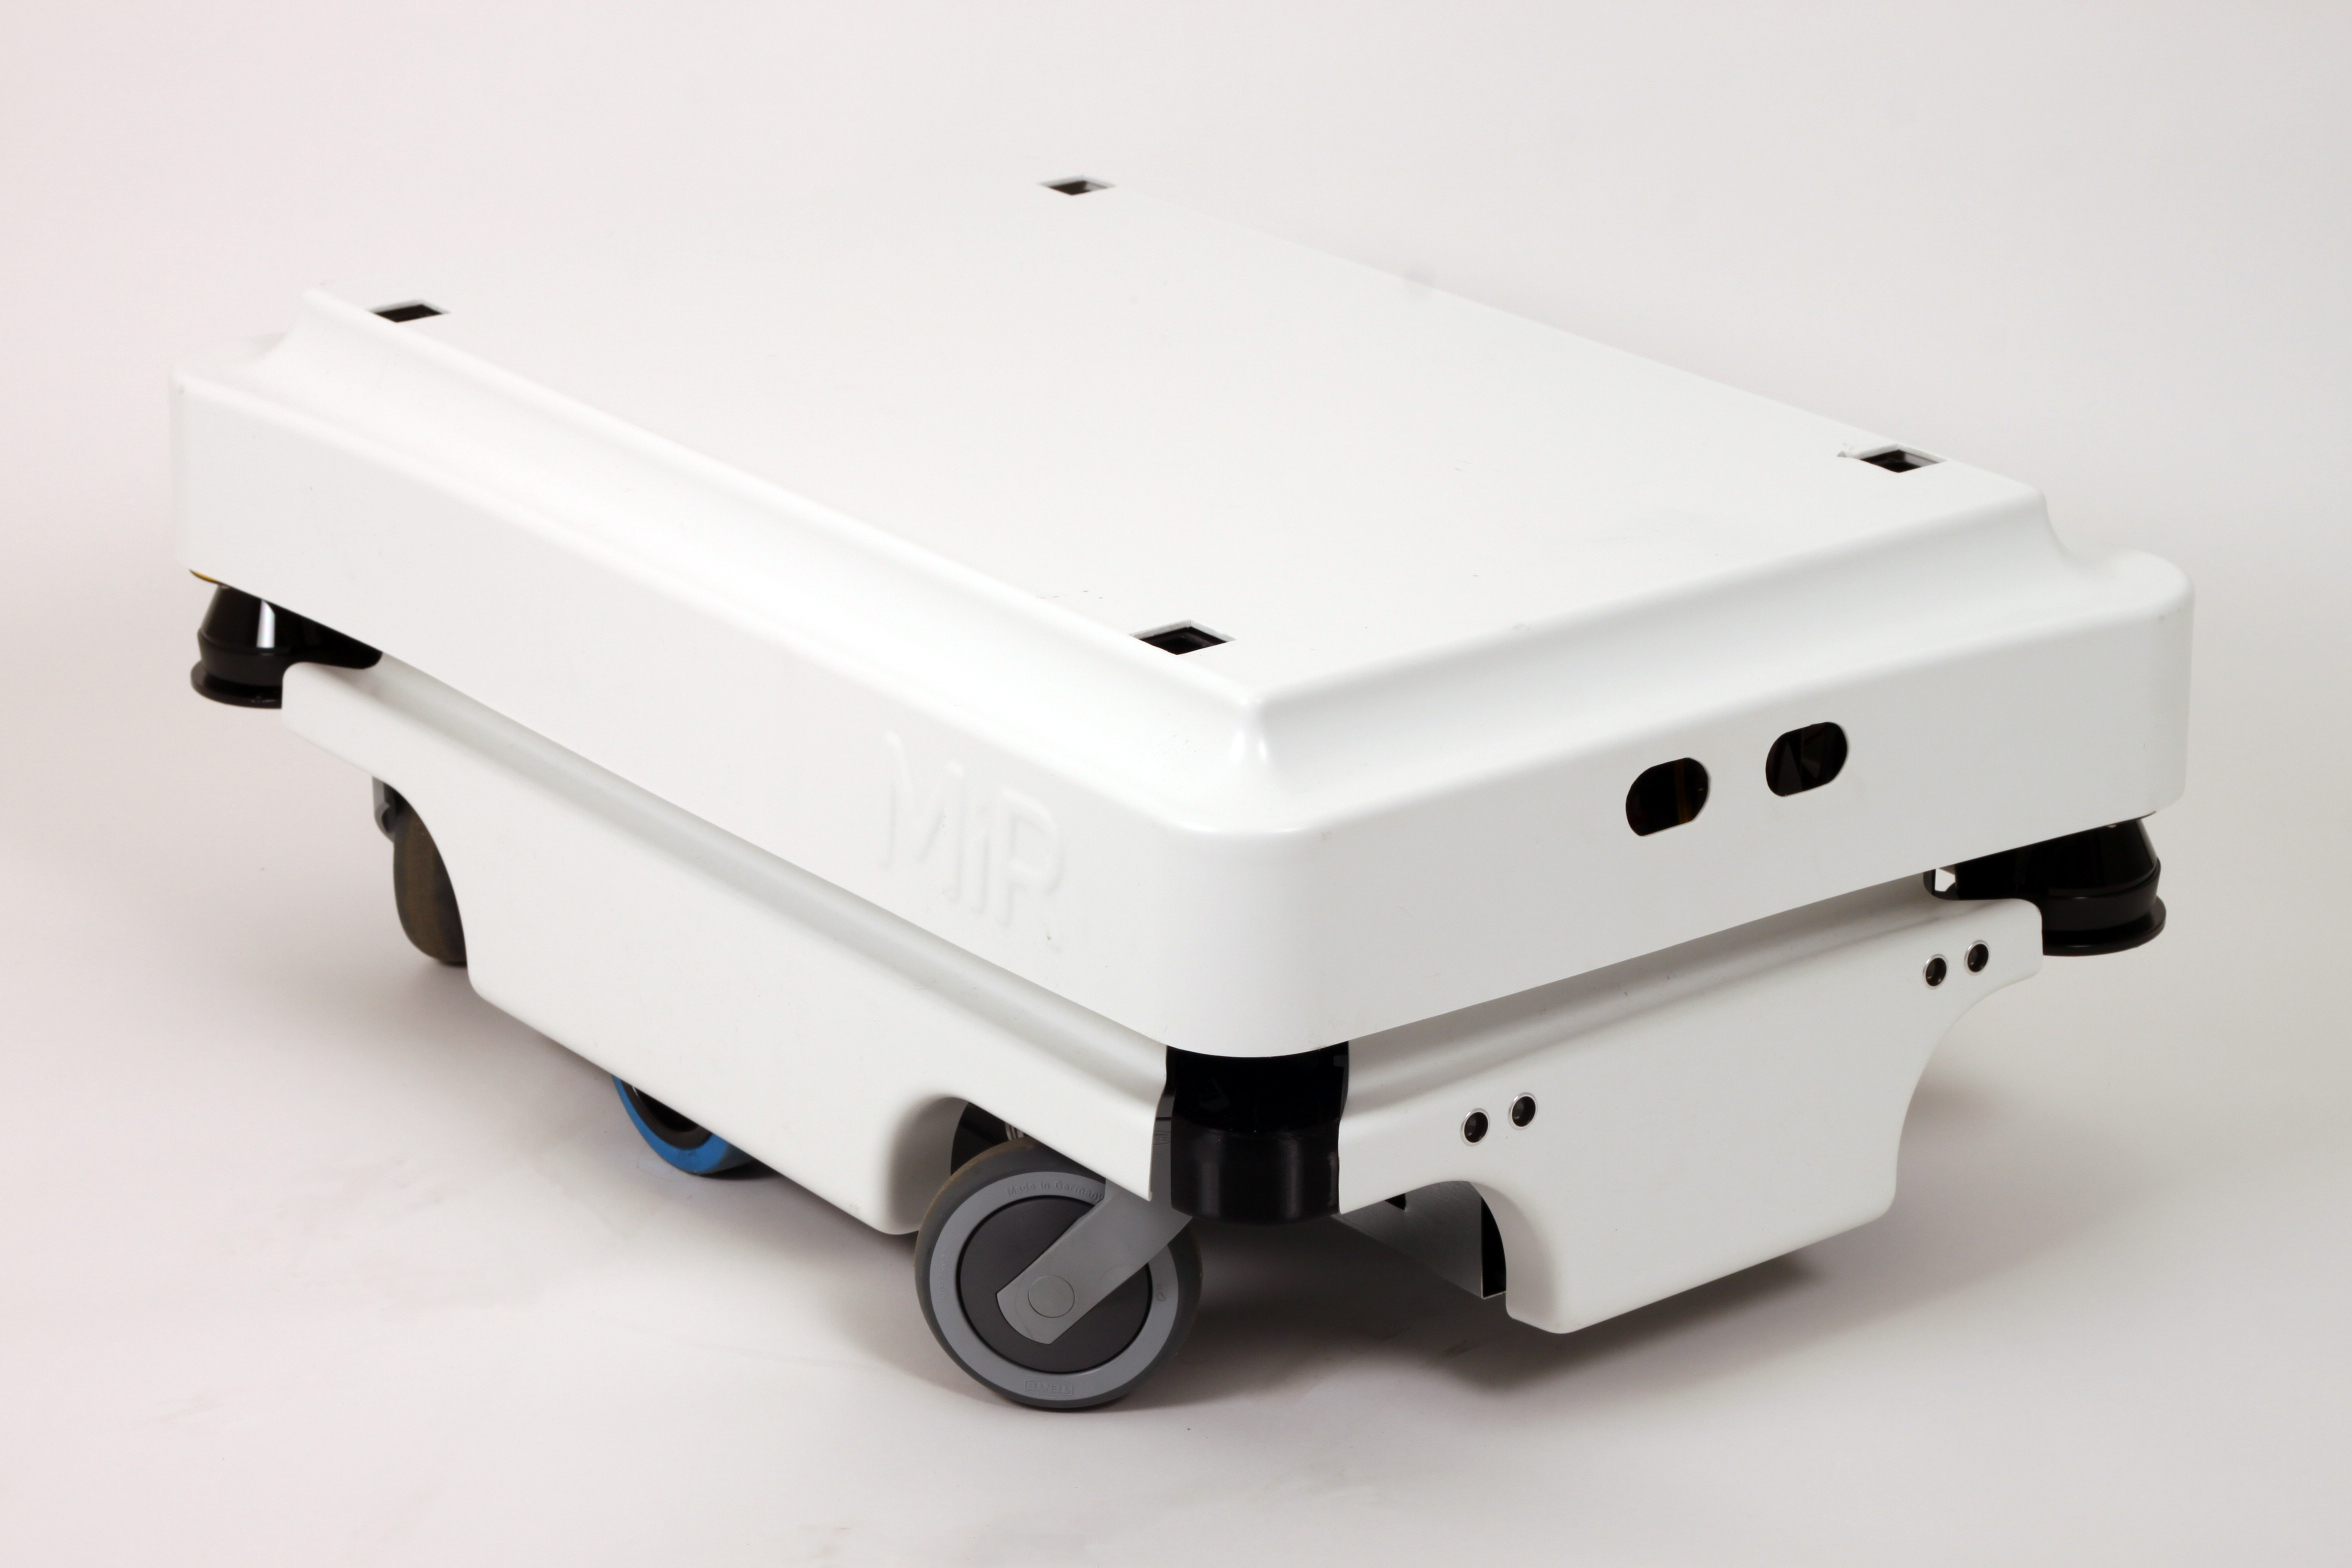
\includegraphics[width=\textwidth]{figures/mobile_mir}
        \caption{MIR 100 by MIR.}
        \label{fig:mobile_mir}
    \end{subfigure}
    \centering
    
    \begin{subfigure}[t]{0.35\textwidth}
        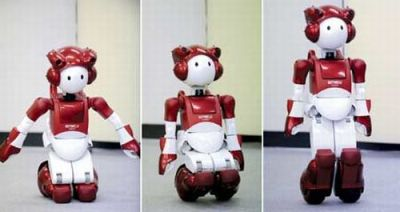
\includegraphics[width=\textwidth]{figures/mobile_hitachi}
        \caption{EMIEW2, by Hitachi.}
        \label{fig:mobile_hitachi}
    \end{subfigure}
    \caption{Examples of wheeled robot platform.}
    \label{fig:mobile_robots}
\end{figure}

Figure \ref{fig:mobile_mir} shows a MIR 100 robot, a state-of-the-art service robot designed for independent transportation and logistics in a dynamic and unpredictable environment..
As a service robot, it must fulfill strict safety standards and guarantee a secure interaction with users and other equipment while accomplishing its tasks.
Thanks to its wheels configuration, it can achieve an agile mobility, fast reaction capacity and a big load capacity.

\hfill

The EMIEW 2, in \ref{fig:mobile_hitachi}, is an example of midpoint between wheeled and legged locomotion.
Although its motion relies on steering wheels, their placement at the end of two leg-like lower-limbs provides with some of the advantages of bipedal motion, such as active suspension or impact absorption.


% subsection the_wheel_in_robotics (end)

\subsection{Achieving legged motion} % (fold)
\label{sub:legged_motion_in_robotics}
In spite of the great successes attained in the field of wheeled-robotics, possible thanks to the development in engines and the increasing computing capacity of embedded processors, mobile robots based on wheels have not been able to achieve performances in motion comparable to the ones found in nature.
Specially in uneven terrains, velocity, maneuverability, and efficiency are still problems under study.
Besides, the absence of wheels in nature as a result of darwinian evolution ultimately led to questioning \cite{dawkins} if they are truly the best mean to overcome the challenges that displacements in uneven, unknown surfaces yield for robots.
In words of Richard Dawkins \cite{dawkins} "[the wheel] is dependent for maximum efficiency on a prior invention – the road (or other smooth, hard surface)". 
Figure \ref{fig:biped_robots} contains three of the most advanced stages in legged locomotion nowadays.
They have been chosen because they are meaningful current paradigms of what brought about the revolution to the leg-based locomotion systems in the 80's: the conjunction between mechanics and control as the producers of the expected behavior \cite{mit_leg_lab1}.

The STARLeth robot in \ref{fig:starleth}, built at the Autonomous System Lab at ETH, is an example of robot legged robot inspired by nature. 
It is meant at proving that versatility, speed, robustness and efficiency can be achieved together in a legged moving platform \cite{starleth}.
But it also represents the control problems arisen from this kind of locomotion, by definition unstable and complex (12 actuated joints and 6 unactuated DOF). 

In Figure \ref{fig:kaist} the Raptor robot created at KAIST is shown.
This robot is inspired in a velociraptor structure and has been able to achieve a top stable speed on a treadmill of 46 $km/h$, making it the current fastest biped robot (although the Cheetah robot by Boston Dynamics has the record as a quadruped).
However, it is discussed here because of its simple bioinspired design, which combines prosthetic blades with a dynamic tail for stabilization and only required two motors.
This makes it a good illustration of the importance of biomechanics in the overall system.

Finally the ATLAS robot by Boston Dynamics, in \ref{fig:atlas}, represents the state of the art in bipedal autonomous platforms handling unknown, rough terrain and its interaction with dynamically changing environment.
This task for a high degree of freedom mobile manipulator as a humanoid requires a very robust interactive motion planning and control in order to quickly carry out its assignment while overcoming unpredicted situations fast and reliably enough.
The ATLAS is a good illustration of the relevance of a robust but flexible and adaptive control architecture for this kind of machines.


\begin{figure}[htb]
    \centering
    \begin{subfigure}[t]{0.40\textwidth}
        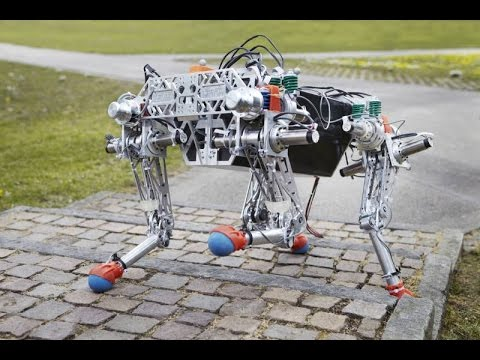
\includegraphics[width=\textwidth]{figures/starleth.jpg}
        \caption{STARLeth}
        \label{fig:starleth}
    \end{subfigure}
    \centering
    \begin{subfigure}[t]{0.40\textwidth}
        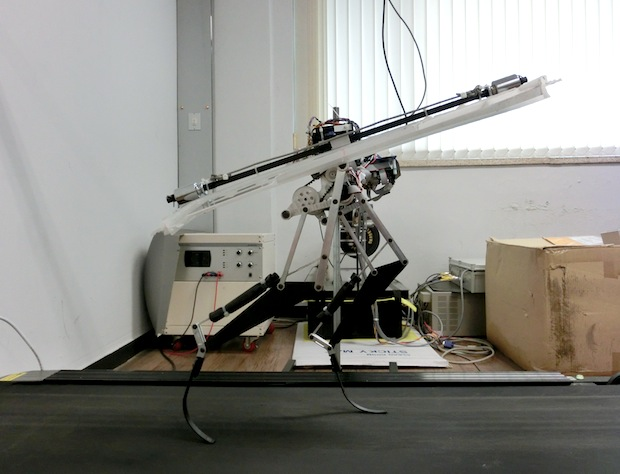
\includegraphics[width=\textwidth]{figures/biped_kaist.jpg}
        \caption{Raptor}
        \label{fig:kaist}
    \end{subfigure}
    \centering


    \begin{subfigure}[t]{0.32\textwidth}
        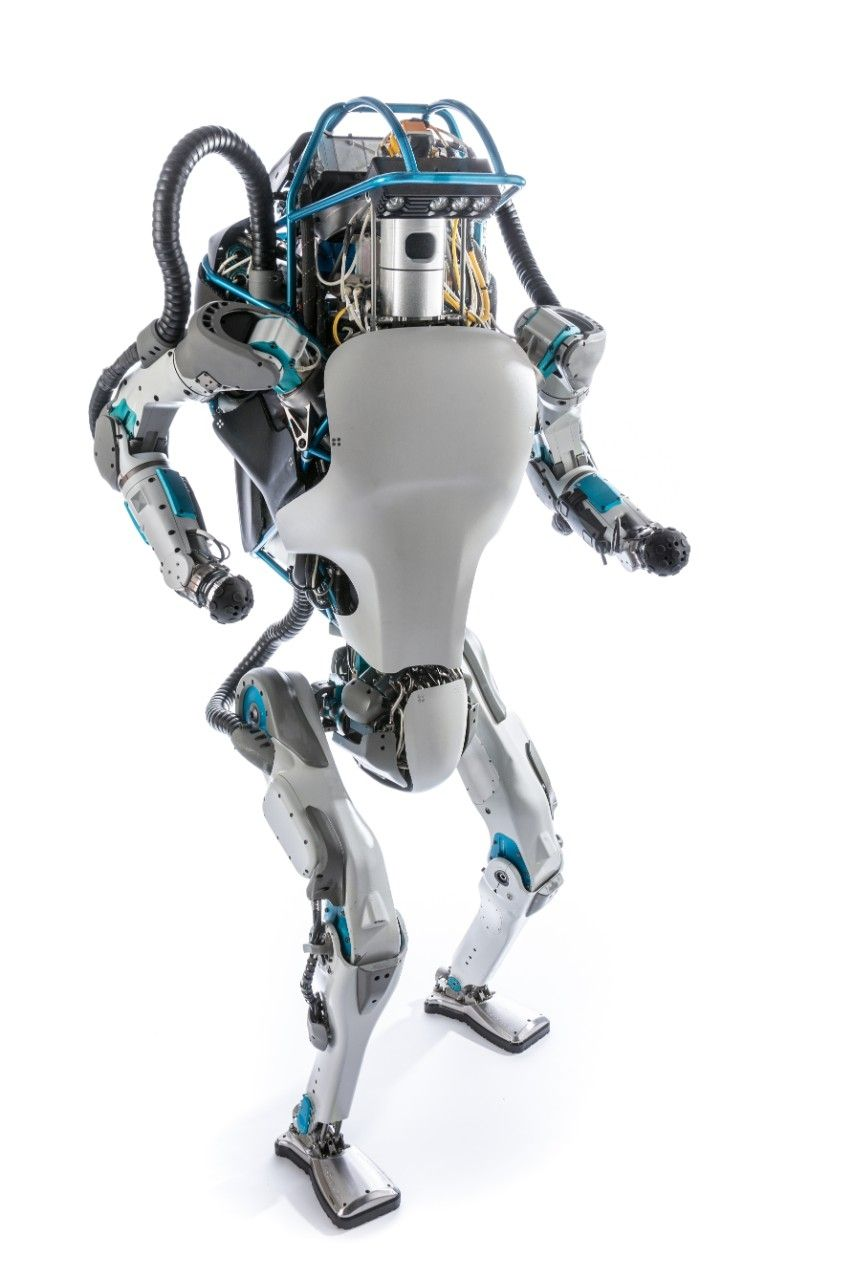
\includegraphics[width=\textwidth]{figures/biped_atlas.jpg}
        \caption{ATLAS}
        \label{fig:atlas}
    \end{subfigure}
    \caption{Examples of legged robot platforms.}
    \label{fig:biped_robots}
\end{figure}


% subsection legged_motion_in_robotics (end)





% section from_the_wheel_to_the_leg (end)
%!TEX root= ../../../report.tex

\section{Biomechanics meets Control} % (fold)
\label{sec:biomechanics_vs_control}
The first attempts to accomplish artificial walking machines in the mid-1950s were based on stiff structures and kinematic control.
There has been more than 60 years of development in several technology fields between them and the current soft, compliant and torque-controlled legged robots.
Among the main advances that gave rise to the evolution of the autonomous walking robots, three considered essential and of great relevance for this thesis are listened in \ref{list:leg_advances} and further discussed here.
Thanks to them, nowadays the research in legged robotics goes hand in hand with the study of biological locomotion systems in the attempt to imitate existing features present in nature.

\begin{itemize}
\label{list:leg_advances}
	\item The realization of the importance that a dynamic and active control has on the walking behavior, as opposed to rigid, kinematics-based motion.
	\item The conception of the embodied AI. The influence of the body in the process of thinking.
	\item The improvements in sensors/actuators performance, material science, embedded computing power and power sources.
\end{itemize}

\subsection{The relevance of body dynamics} % (fold)
\label{sub:dynamics_control}
Stiff position control for kinematic trajectory planning has lately demonstrated impressive capabilities for instance during the last DARPA learning locomotion challenge.
However, the limitations of this kind of control such as the need of a very detailed knowledge  about both the robot state vector and the environment have been also exposed.
Thus, it seems clear that the solution for robust and adaptive motion platforms has to go through the development of dynamics-based control models.
The first big steps in dynamic legged locomotion control took place in the 90's in the Leg Laboratory, at the MIT Artificial Intelligence Laboratory carried out by Marc Raibert and his team.
Their findings about the importance of active balance for stability and the possibility of creating simple and generalizable control algorithms for complex dynamic legged systems \cite{mit_leg_lab1} pushed the development of walking robots to a new stage.
Besides, they were among the pioneers in the realization of the influence of the mechanical design together with the control in the generation of complex behaviors in locomotion.
A paradigmatic example of the importance of the biomechanics and the body dynamics in the control of machines intended for locomotion is the well-known passive walker developed by McGeer \cite{passive_walking} and shown in \ref{fig:passive_walker}. 
The achievement of a human-like, efficient walking behavior without any kind control structure gave birth to the concept of morphological computation.

% subsection dynamics_control (end)
\begin{figure}[h]
	\centering
	\begin{subfigure}[b]{0.45\textwidth}
        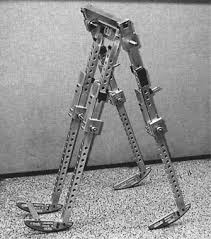
\includegraphics[width=\textwidth]{figures/passive_walker.jpg}
        \caption{McGeer's passive walker}
        \label{fig:passive_walker}
    \end{subfigure}
    \begin{subfigure}[b]{0.45\textwidth}
        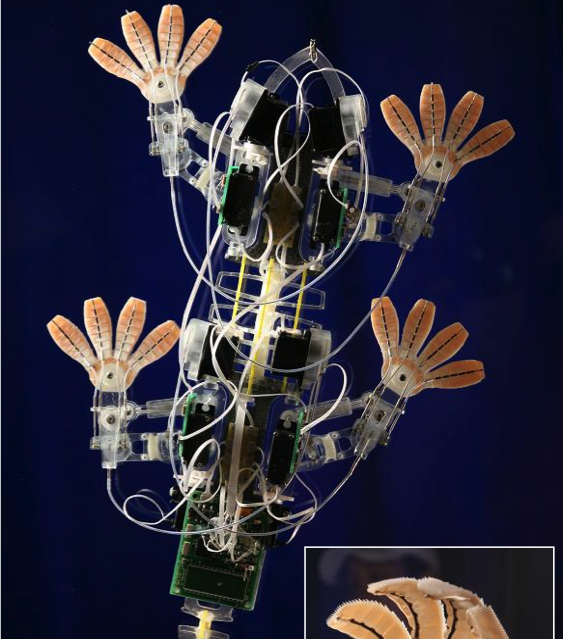
\includegraphics[width=\textwidth]{figures/Stickybot.jpg}
        \caption{Stickybot robot, Standford University}
        \label{fig:stickybot}
    \end{subfigure}
\caption{Examples of bio inspired mechanics in locomotion}
\label{fig:figure1}
\end{figure}

\subsection{Embodied AI and locomotion} % (fold)
\label{sub:the_embodiment_}
The embodiment concept came up in the Artificial Intelligence field in the 1980's as a mean to explore the influence of the body and its characteristics in the process of thinking. 
Its aim could be expressed as the search for the answer to the question, in the very convenient words of Rolf Pfeifer and Fumiya Iida, "How does walking relate to thinking?".
As introduced in \cite{pfeifer}, the original goal of AI the understanding of natural forms of intelligence that have more to do with the interaction with the real world rather than the only development of computer algorithms.

The advent of this new approach in AI caused by itself an enormous boost in the field of locomotion in robotics since it made researchers start working with mobile robots.
"The general initial conviction that locomotion and orientation were the underlying driving forces in the development of cognition, in the evolution of the brain, led to the general use of the already available wheeled robots" \cite{pfeifer}.
In the seek of an answer to the famous question "Why don’t plants have brains?", by D. Wolpert, the belief that the reason could be their incapacity for displacement led to an increasing use of mobile robots as a research tool.

Besides, the embodied AI brought about the turn to nature for inspiration in biological systems under the belief that the results of Darwinian evolution and the principle of ecological balance had created systems of greater complexity and efficiency worth studying and mimicking.
With all this, it came the understanding that complex behavior could arise from the synergistic combination of simple algorithms and the physical characteristics of the body.
Since then, mechanical compliance in the actuation, soft materials and bio inspired controllers such as CPGs for instance have been widely studied and implemented in walking machines. 
An example of this concept is the Stickybot, created in the Biomimetics and Dexterous Manipulation Lab at Standford University and shown in Figure \ref{fig:stickybot}.
% subsection the_embodiment_ (end)

\subsection{The advancement of hardware} % (fold)
\label{sub:the_advances_in_hardware}
The early timeline of the evolution in the technology utilized in biped robotic systems can be analyzed taking a look at the progression of the humanoid robots at Waseda University in Japan, in the Humanoid Research Laboratory.
In the late 1960's, Ichiro Kato and his team created the WAP-1, the first version of their first generation of humanoid robots, and the WAM-1 \ref{fig:waseda_robot1}, matching the launching of the first microprocessors.
The WAP-1 robot was moved by very slow pneumatic artificial muscles, first developed in the 1950's but not widely commercialized until the beginning of the 80's, and had to be connected to a large external computer frame for its control. 
Later version WAP-2 and WAP-3 incorporated controller-based memory and PWM-driven actuators, created at the end of the 1960's, that allowed to reach three-dimensional walking at near human-like locomotion speeds for the first time in history.
Kato also created the first full-size humanoid robot, the Wabot-I, and since the beginning of the 80's his group and him applied for the first time 16-bit microcomputers (introduced in 1973) to the implementation of quasy-dynamic walking control \cite{biped_robots_history}.
On of the latest achievements of Kato Laboratory is the WABIAN-2R, in \ref{fig:waseda_robot2}.

\begin{figure}[h]
	\centering
    \begin{subfigure}[b]{0.4\textwidth}
        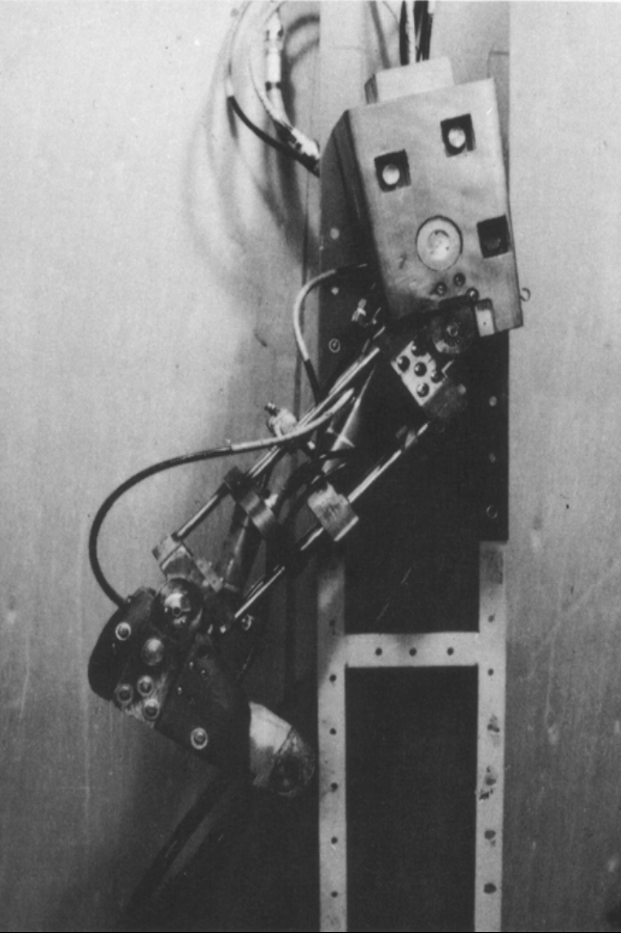
\includegraphics[width=\textwidth]{figures/waseda1.pdf}
        \caption{WAM-1 (1966)}
        \label{fig:waseda_robot1}
    \end{subfigure}
    \centering
    \begin{subfigure}[b]{0.4\textwidth}
        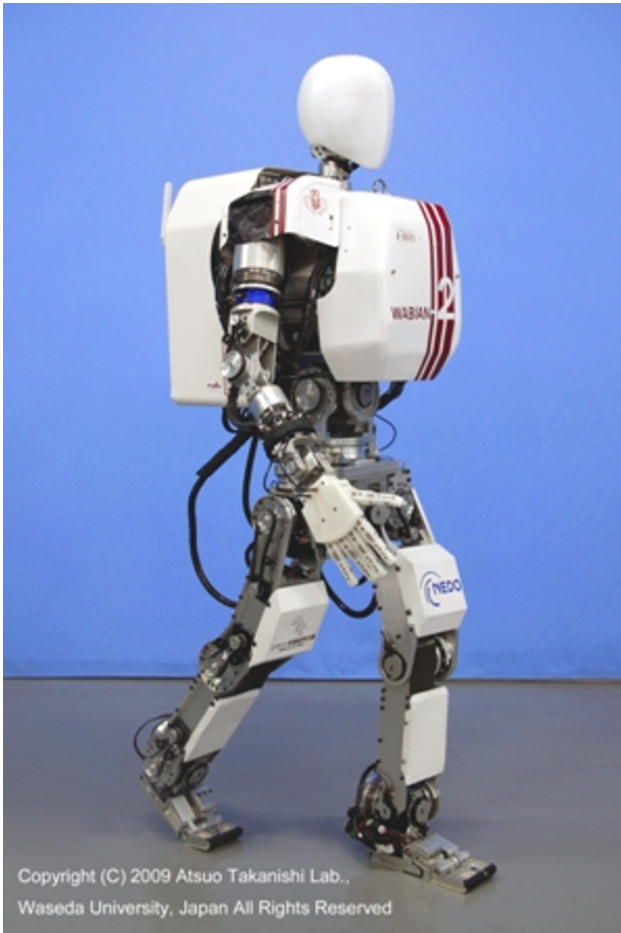
\includegraphics[width=\textwidth]{figures/waseda2.pdf}
        \caption{WABIAN-2R (2006)}
        \label{fig:waseda_robot2}
    \end{subfigure}
\end{figure}

The above is just an example of how during the last two decades of the 20th century and the beginning of the 21st, the progresses in sensing, actuation and control has largely influenced the development of legged locomotion in robotics.
However, despite the latest and impressive enhancements in mechatronics, its evolution continues presenting challenges for the advancement of autonomous biped robots.
Nowadays, the main requirements from a hardware point of view are listed in \ref{list:hardware_challenges} as per \cite{biped_robots_history}.

\begin{itemize}
	\item Energy-efficient and high-performance actuators with high torque-to-weight ratio and high torque-to-volume ratio.
	\item Highly reliable while economical sensors.
	\item Lightweight but mechanically strong materials for construction of the structure and mechanism.
	\item Fast, high computing power, and economical dedicated computer system robust against hostile situations of nature.
	\item Lighter power sources with greater autonomy.
\label{list:hardware_challenges}
\end{itemize}

In spite of this, it seems that the progress in legged autonomous systems will come from the hand of the introduction in the robotics field of recent areas in science as nanotechnology or smart materials.
Together with this, the new findings in microelectronics and the miniaturization of computers and batteries will help overcome the current challenges.


% subsection the_advances_in_hardware (end)


% section biomechanics_vs_control (end)
%!TEX root= ../../../report.tex

\section{The next generation of bipeds} % (fold)
\label{sec:the_next_generation_of_bipeds}
It appears clear now that the evolution of bipedal locomotion has in the last decades suffered a wide-reaching change in its conditions with the entrance on the stage of robotics science and its research in walking machines.
It still stands difficult, however, to foresee the paths that the advancements in artificial bipedalism will take without the risk of getting lost in speculations.
Notwithstanding, the latest breakthroughs yield reasons to believe that the next generation of walking machines will resemble more and more the physiological designs developed by nature, although only to the extent that the state-of-the-art mechantronics allows.
This last fact entails that a complete imitation of living biological structures is yet out of the reach of engineering, thus making its goal not to just copy, but to understand the underlying principles that drive biology and transfer them to the new synthetic creations with the existing technology.



However, the latest advances in some of the youngest areas of the engineering seem to be close to bring about a change in the so far unaltered rules of the game.
The progresses in AI and in the design of genetic algorithms have arisen the possibility of not only striving for mimicking nature, but also replicating its fundamental processes, artificially accelerating and modifying them.
In the next decades, nature could stop being the only motor of evolution and from there, the possibilities are boundless.

% section the_next_generation_of_bipeds (end)
%%!TEX root = ../../report.tex
\chapter{State of the art} % (fold)
\label{cha:state_of_the_art}
This chapter contains a concise overview of some of the major, and more relevant for this thesis, advances in artificial legged locomotion in the past 60 years.
A brief prelude of the emergence and evolution of natural, limb-based terrestrial motion and more in detail bipedalism is presented.
It is followed by a short introduction of some of the history and results from the union between the engineering field and the study of motion and legged systems. 
From the first, ancient mobile artifacts and prosthesis to the current, most advanced devices in robotics.
It continues with an exposition of three of the most pertinent breakthroughs in modern technologies that allowed to reach the current state of the art in modern autonomous walking robots.
And it finishes with a quick look to the future of the bipedal locomotion.

\input{chapters/cha_state_of_the_art/Sections/sec_bipedalism_intro}
\input{chapters/cha_state_of_the_art/Sections/sec_wheel_to_leg}
\input{chapters/cha_state_of_the_art/Sections/sec_biomechanics_vs_control}
\input{chapters/cha_state_of_the_art/Sections/sec_next_generation}
%\input{chapters/cha_state_of_the_art/cha_state_of_the_art}
%\input{chapters/cha_state_of_the_art/Sections/sec_theoretical_background}
%\section{Theoretical background}



%But it has been in the last 30 years of the past century when the robotics field has started to focus on accomplishing bipedal locomotion, being the first model the WAM-1, built at Waseda University in 1967 \cite{}.
% Since this robot, the evolution of the platforms targeted at mimicking human locomotion has rapidly achieved great successes, which can be exemplified in robots as ASIMO, MABEL or BioBiped \cite{mabel}, \cite{biobiped}, %\cite{}.  
% However, even though the generation of stable walking gaits for biped platforms seems to have reached a next stage with the latest Atlas robot, the variances in kinematics, kinetics and control required for running and for the transition between the walking and running gaits still set out unsolved challenges.
% Besides, differences in energy consumption and balance control or trajectory generation still remain noticeable when comparing the performance of humanoid robots and humans \cite{h7}.

% In order to contribute to the study of stable walking and running gaits generation in bipedal robots, and aiming at providing a new tool to gain new insights on the transition between these gaits, this project offers a new robotic platform for continuing the research in these areas at the University of Southern Denmark.
% The current bipedal robot being utilized at the AI department at the Mærsk Mc-Kinney Møller Institute to benchmark neural controllers for locomotion is the DACbot walking robot, a next generation of RunBot \cite{runbot1} \cite{runbot2}.
% The limitations of this model when trying to approach human-like gait include among others the lack of actuated ankles or compliance in other joints besides the ankles. 
% Furthermore, its fixed structure and the way it was manufactured make modifications for different experiments or even repairs a hard task.
% A new bipedal platform offering a structure easy to modify and repair, low-cost, fully actuated and whose compliant components can be reconfigured, could be a valuable instrument for future studies.
% The RuBi robot, introduced here, wants to be presented as a mean to overcome the above mentioned restrictions and provide these new features. 
% Besides, the possibilities arisen from having two different study platforms in the department include being able to test neural controllers in different robots to observe their adaption, for instance.



%\section{Current research}
% chapter state_of_the_art (end)
%%!TEX root = ../../../report.tex

\section{Theoretical background}
\label{sec:theoretical_background}

%\section{Theoretical background}



%But it has been in the last 30 years of the past century when the robotics field has started to focus on accomplishing bipedal locomotion, being the first model the WAM-1, built at Waseda University in 1967 \cite{}.
% Since this robot, the evolution of the platforms targeted at mimicking human locomotion has rapidly achieved great successes, which can be exemplified in robots as ASIMO, MABEL or BioBiped \cite{mabel}, \cite{biobiped}, %\cite{}.  
% However, even though the generation of stable walking gaits for biped platforms seems to have reached a next stage with the latest Atlas robot, the variances in kinematics, kinetics and control required for running and for the transition between the walking and running gaits still set out unsolved challenges.
% Besides, differences in energy consumption and balance control or trajectory generation still remain noticeable when comparing the performance of humanoid robots and humans \cite{h7}.

% In order to contribute to the study of stable walking and running gaits generation in bipedal robots, and aiming at providing a new tool to gain new insights on the transition between these gaits, this project offers a new robotic platform for continuing the research in these areas at the University of Southern Denmark.
% The current bipedal robot being utilized at the AI department at the Mærsk Mc-Kinney Møller Institute to benchmark neural controllers for locomotion is the DACbot walking robot, a next generation of RunBot \cite{runbot1} \cite{runbot2}.
% The limitations of this model when trying to approach human-like gait include among others the lack of actuated ankles or compliance in other joints besides the ankles. 
% Furthermore, its fixed structure and the way it was manufactured make modifications for different experiments or even repairs a hard task.
% A new bipedal platform offering a structure easy to modify and repair, low-cost, fully actuated and whose compliant components can be reconfigured, could be a valuable instrument for future studies.
% The RuBi robot, introduced here, wants to be presented as a mean to overcome the above mentioned restrictions and provide these new features. 
% Besides, the possibilities arisen from having two different study platforms in the department include being able to test neural controllers in different robots to observe their adaption, for instance.



%\section{Current research}
% chapter state_of_the_art (end)
%%!TEX root = ../../../report.tex

\section{Theoretical background}
\label{sec:theoretical_background}

%\section{Theoretical background}



%But it has been in the last 30 years of the past century when the robotics field has started to focus on accomplishing bipedal locomotion, being the first model the WAM-1, built at Waseda University in 1967 \cite{}.
% Since this robot, the evolution of the platforms targeted at mimicking human locomotion has rapidly achieved great successes, which can be exemplified in robots as ASIMO, MABEL or BioBiped \cite{mabel}, \cite{biobiped}, %\cite{}.  
% However, even though the generation of stable walking gaits for biped platforms seems to have reached a next stage with the latest Atlas robot, the variances in kinematics, kinetics and control required for running and for the transition between the walking and running gaits still set out unsolved challenges.
% Besides, differences in energy consumption and balance control or trajectory generation still remain noticeable when comparing the performance of humanoid robots and humans \cite{h7}.

% In order to contribute to the study of stable walking and running gaits generation in bipedal robots, and aiming at providing a new tool to gain new insights on the transition between these gaits, this project offers a new robotic platform for continuing the research in these areas at the University of Southern Denmark.
% The current bipedal robot being utilized at the AI department at the Mærsk Mc-Kinney Møller Institute to benchmark neural controllers for locomotion is the DACbot walking robot, a next generation of RunBot \cite{runbot1} \cite{runbot2}.
% The limitations of this model when trying to approach human-like gait include among others the lack of actuated ankles or compliance in other joints besides the ankles. 
% Furthermore, its fixed structure and the way it was manufactured make modifications for different experiments or even repairs a hard task.
% A new bipedal platform offering a structure easy to modify and repair, low-cost, fully actuated and whose compliant components can be reconfigured, could be a valuable instrument for future studies.
% The RuBi robot, introduced here, wants to be presented as a mean to overcome the above mentioned restrictions and provide these new features. 
% Besides, the possibilities arisen from having two different study platforms in the department include being able to test neural controllers in different robots to observe their adaption, for instance.



%\section{Current research}
% chapter state_of_the_art (end)
    %!TEX root = ../../report.tex
\chapter{Conception and initial analysis} % (fold)
\label{cha:analysis}
The process of designing and constructing a bipedal robot as the presented here is a task of great magnitude in which a big set of parameters has to be analyzed and determined aiming at the most optimal solution possible\footnote{Optimality here is measured in terms of the aimed goals, described in \ref{sec:goals}.}.
The important role of the geometrical and inertial mechanical parameters in locomotion control was first proved by \cite{passive_walking}, and their relevance deserves a careful study.
Thus, the sections in this chapter contain the conceptual presentation of a set of design criteria and first approaches to the construction of the RuBi prototype arisen from the study of these parameters.

%!TEX root= ../../../report.tex

\section{Bipedal locomotion} % (fold)
\label{sec:bipedal_walking_and_running_gaits}
This section contains a superficial comparative study of the characteristics of the motion patterns in human walking and running.
The reason is to help justify in the following chapters the decisions taken during the design towards the generation of these gaits.

Although walking and running motion patterns in humans might resemble each other at first glance, they contain important variations that imply that a robot able to walk at a certain speed is not necessary capable of running at the same speed, or running at all.
The existence of the so-called "flight phase" in running but not in walking cycles is the main difference between them.
This phase comprises the period in which there is no contact between the feet and the ground and causes the main variations in energy and trajectory generation.

\subsection{Walking and running gaits comparison} % (fold)
\label{sub:walk_and_run_comparison}
The differences in both joint kinematics and kinetics between both patterns emerged from the distinction mentioned are studied in \cite{grimmer}, Manuscript I, for a wide range of speeds.
From the cited paper it can be seen that the joint positions for a whole cycle in both walking and running patterns are very similar, specially for hip and knee.
Furthermore, the joint velocity profiles have almost the same shape but differ in the magnitudes, being higher the angular speeds reached for running.
Similar conclusions can be extracted from a quick comparison between the torque and power profiles in a running and walking cycle.
While the shapes of the functions for the three joints are very alike, with the biggest differences for the ankle, the values of the curve are in average smaller for human walking than for running.
As expected, the conclusion is that higher requirements for joint speed, torque and power are expected for running, specially for the knees and the ankles.
Besides, the foot strike and impact forces during the landing phase in both cases change, both in intensity and profile.
% subsection walk_and_run_comparison (end)

% section bipedal_walking_and_running_gaits (end)
%!TEX root = ../../../report.tex

\section{Geometrical dimensions of the frame} % (fold)
\label{sec:dimensions}
The selection of the final dimensions of RuBi corresponds to an iterative process in which power requirements and achieving human-like kinematics have been the main constraints when assessing the size of the robot.
A first approach was taken from \cite{grimmer}, Manuscript I, where normalized values of power required per joint and per kilogram of the structure can be found.
The first iteration targeted a robot of dimensions $m = 1Kg$ and length from the hip joint to the tip toes of $L = 0.6 m$ for a fully stretched leg.
The final parameters from the last iteration can be found in ***%***chapter Results

Once estimated an overall length of the structure, an initial value of the dimensions of each link were decided to be obtained based on the German section of the ISO 7250-2 \cite{iso_measurements} and the DIN 33402-2 \cite{din_measurements1} norms, following the idea of mimicking human-like motion as closely as possible.
These two norms are standard references in industry and were considered a general enough source of information.
Figure \ref{fig:human_measurements} depicts some of the human dimensions extracted from the norms and applied to the design of RuBi.
Their names and values for male between 18-65 year old and in percentile 50 can be found in table \ref{tab:din_proportions}.

\begin{figure}[h]
	\centering
	\begin{subfigure}[b]{0.3\textwidth}
        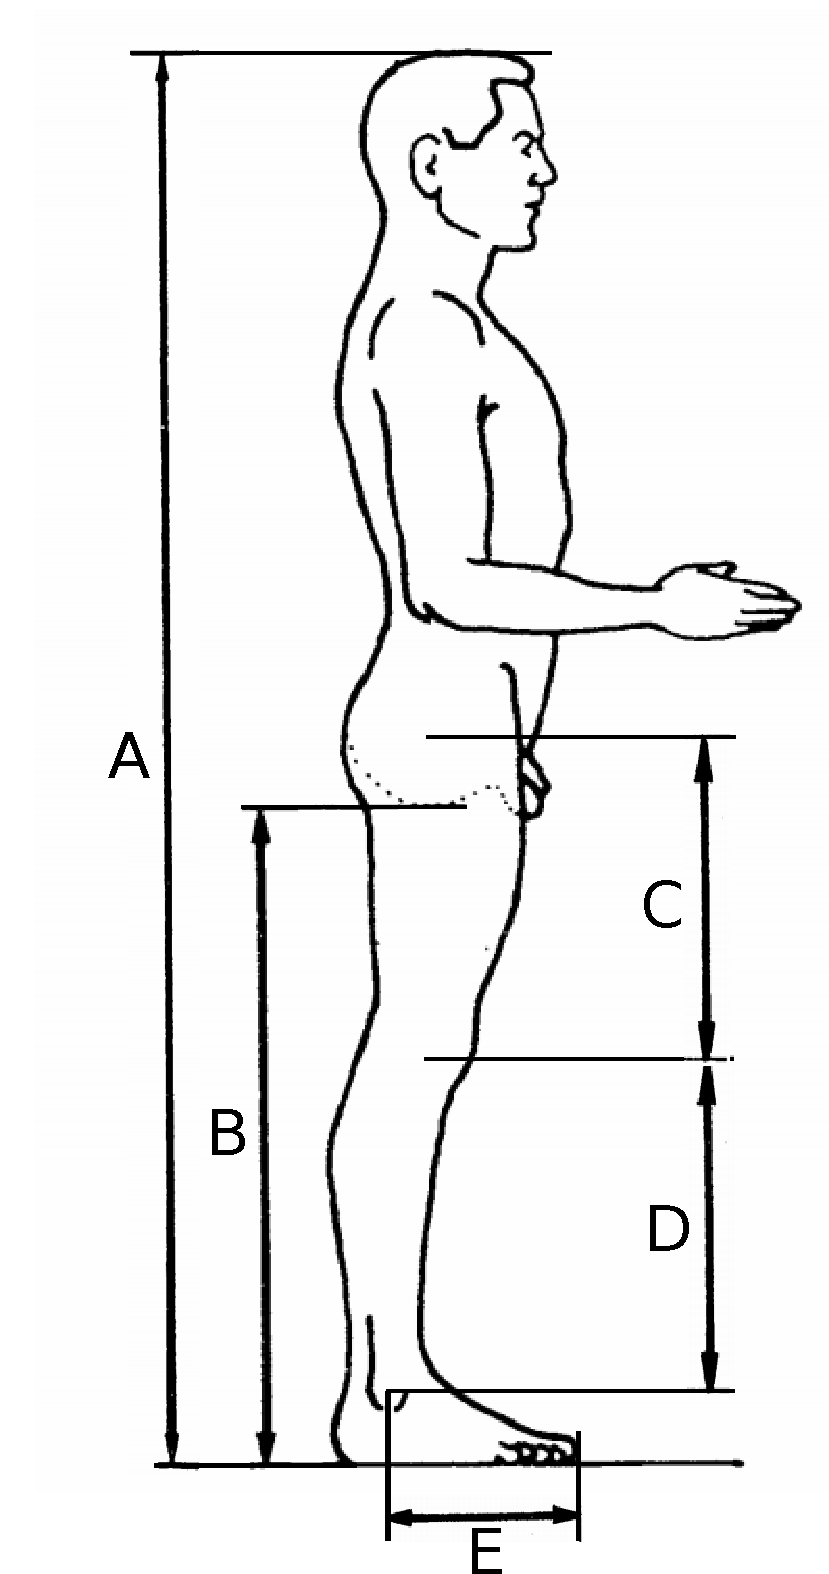
\includegraphics[width=\textwidth]{figures/din_measurements.pdf}
        \caption{Left foot}
        \label{fig:din1}
    \end{subfigure}
    \begin{subfigure}[b]{0.4\textwidth}
        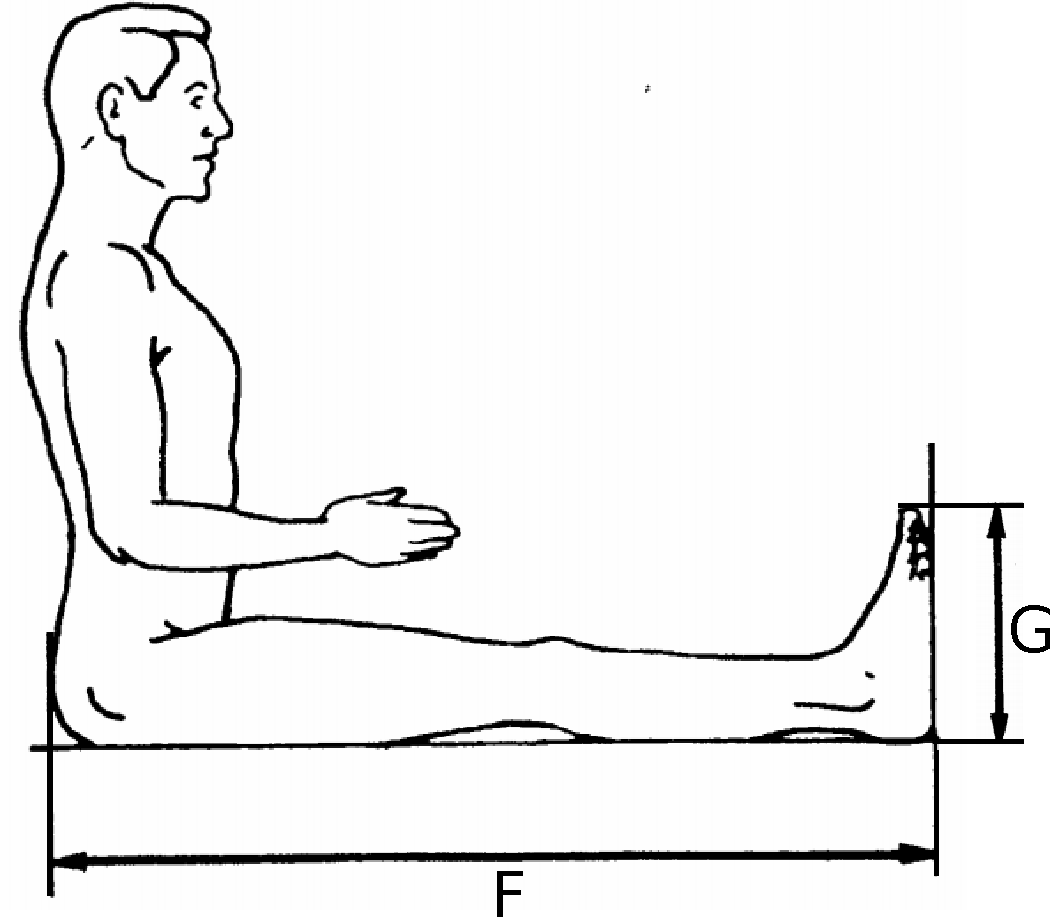
\includegraphics[width=\textwidth]{figures/din_measurements2.pdf}
        \caption{Hip}
        \label{fig:din2}
    \end{subfigure}
	\caption{Lower body measurements used for RuBi. Picture adapted from \cite{din_measurements1}.}
	\label{fig:human_measurements}
\end{figure}


\begin{table}
\begin{center}
	\begin{tabular}{c | c | c | c}
	  Index & Definition & Value & \% of Stature \\
	  \hline
	  A & Stature (body height) & ** & 100 \\
	  B & Crotch height & ** & ** \\
	  C & Femur height & ** & ** \\
	  D & Tibial height & Not in norm & **\\
	  E & Ankle-toe tip distance & Not in norm & ** \\
	  F & Buttocks-leg length & ** & ** \\
	  G & Sole length & ** & **
	\end{tabular}
	\caption{Human proportions from DIN 33402-2}
	\label{tab:din_proportions}
\end{center}
\end{table}

\subsection{Limbs length} % (fold)
\label{sub:limbs_lengths}
The dimensions needed to create a simplified model of one leg are the limbs lengths, which are the straight line distances measured from two consecutive joints.
They have been called $l_{i}$ where $i$ is the robot link + joint as per table \ref{tab:limb_index} and can be seen in Figure \ref{fig:kinematics}.
However, the norm does not determine all of them.

\begin{table}
\begin{center}
	\begin{tabular}{c | c | c}
	  $l_{i}$ & Limb \\
	  \hline
	  $l_{1}$ & Hip + thigh & C \\
	  $l_{2}$ & Knee + Foreleg & D\\
	  $l_{3}$ & Ankle + foot & E 
	\end{tabular}
	\caption{Limbs index}
	\label{tab:limb_index}
\end{center}
\end{table}

Since $C$ and $E$ are not standard measurements in industry, they have been obtained as follows:

\paragraph{The Femur height}
The crotch height, denoted as $B$ in the figure, has been averaged with the buttocks-leg length and the tibial height + an empirical approximation of the height of the ankle have been subtracted from the result, obtaining $C$.

\paragraph{The ankle-toe tip distance}
Since this distance is not standard either, it has been obtained once again adjusting the sole length with empirical measurements.
% subsection limbs_lengths (end)

\subsection{Hip and sole width} % (fold)
\label{sub:subsection_name}
The hip width sitting, as defined in the norm and for the same sample group than before, has been used as starting point to define the final width of the structure of the hip.
This standard measurement has been scaled down to a human of length L from hip joint to toe tip, which would correspond to $L=C+D+E$, using the proportion between stature and lower body lengths, also obtained from the norm.
The same process has been conducted to calculate the implemented width of the foot sole.

% subsection hip_sole_width (end)

No other standard measurement has been used as reference for the design, such as thigh or lower leg circumferences, since they do not affect the kinematics of the structure although they have a big influence in its dynamics.
The criteria followed to model the dynamics of the robot is explained in \ref{sec:physical_properties}.


%% Here we just describe the process followed to obtain the final dimensions. 
%% The final results are shown in Chapter Results --> add tables and Froude number calculus


% section dimensions (end)
%!TEX root = ../../../report.tex

\section{Inertial dimensions of the frame} % (fold)
\label{sec:physical_properties}
This section presents the theoretical guidelines followed during the design of RuBi regarding its dynamic model.
The calculations carried out are to be found in chapters \ref{cha:mathematical_model} and \ref{cha:design}. 
The determination of the geometrical dimensions for a robot model is in general a deterministic task in which all the parameters can be selected without dependencies or limitations.
However the inertial parameters of a robot will be the result of the selection of these dimensions, together with the materials utilized for the implementation and the configuration of the elements on the structure, among others.
Here, the goal of the adjustment of the final inertial parameters is not to mimic the dynamics of human legs as with the kinematics, but to reduce the power requirements for locomotion while ensuring robustness and reliability.
The main inertial parameters object of study here are the mass of the links, the positions of their CoM and their inertia moments.
Other parameters with an influence in the model dynamics such as friction forces or delays introduced by transmissions are not discussed here due to the complexity of its determination at this stage of the project.

\subsection{Mass of the links} % (fold)
\label{sub:mass_of_the_limbs}
The mass of each limb $i$ will depend on the materials used, their geometry and their density together with any other component added to the link (actuators, electronics, transmissions).
As explained before, keeping the overall mass of the frame as low as possible while guaranteeing the fulfillment of all the structural requirements, such as resistance and resilience, has been one of the main goals of the analyses conducted in the design of RuBi.
This criteria led to the allocation of the embedded electronics off the robot and aim at small electric actuators as the lightest possible solution for the actuation. 
The calculations to select the limb materials and profiles are to be found in \ref{sub:limb_profile}.
The final values of mass per limb have been obtained as an approximate sum of the components that constitute them, due to the complexity of measuring them directly or using system identification techniques. 
They can be seen in \ref{tab:limb_physical_properties} and they have been assumed to be concentrated in the CoM of each link for the computation of the dynamic model.

% subsection mass_of_the_limbs (end) 
\vfill
\subsection{Mass distributions} % (fold)
\label{sub:centers_of_mass}

\paragraph{Limbs center of mass} % (fold)
\label{par:limbs_center_of_mass}
The position of the center of mass (CoM) of each limb referred to its joint rotational axis is a function of its masses, their distributions and its geometry.
Their coordinates are given referred to a local reference frame attached to each joint, with its $Z$ axis perpendicular to the sagital plane and its $X$ and $Y$ axes parallel to its equivalents in the main reference frame in the hip, shown in Figure \ref{fig:kinematics}.
Its direct influence in the dynamics of the system is shown in \ref{sec_dynamic_model}, equation \ref{eq:N-E_eq1}.
The coordinates of the CoM of the limbs have been estimated during the design through the 3D CAD design software tool SolidWorks \cite{solidworks}.
Their final values can be found in \ref{tab:limb_physical_properties}.

% paragraph limbs_center_of_mass (end)

\paragraph{Center of mass of the frame} % (fold)
\label{par:center_of_mass_of_the_frame}
The location of the frame center of mass plays a very important role in the stability of the robot \cite{rojas}.
Its theoretical placement when standing still should be in the sagital plane of the structure, as close to the hip as possible, similar to humans (accounting that there is no torso).
A robust locomotion should result in a controlled and limited motion of the CoM. 
A high positioning of the CoM in the structure would make it more sensitive to the actuators influence, allowing a better balance control, while a lower placement in the structure could increase its robustness against inertial phenomenas.
The trade-off between these two criteria has been tried to be found.
As for the limbs, the coordinates of the CoM of the structure have been computed through SolidWorks and their final values can be found in %\ref{} reference to Results table and Implementation section

% paragraph center_of_mass_of_the_frame (end)

% subsection centers_of_mass (end)

\subsection{Moments of inertia} % (fold)
\label{sub:moments_of_inertia}
The inertia tensor of each limb will be the result of their distribution of masses with respect to the joint axis.
Since the kinematics analysis of the robot has been reduced to a planar case for both legs, as discussed in \ref{sec_kinematic_model}, the tensors have been reduced to a scalar value, their $I_{zz}$ component for the defined reference system.
The influence of the inertia moments of the limbs in the dynamics of the system can be seen in equation \ref{eq:N-E_eq1} where is, as per definition, the proportion between angular acceleration around the axis and torque applied.
This relationship yields another design criteria for the robot: the minimization of the inertia moments of the limbs in order to reduce the required torque applied for moving the limbs.
As for the previous magnitudes, the final inertia moments have been calculated with the CAD model in SolidWorks, and can be found in \ref{tab:limb_physical_properties}.
Their role in the simulation model developed in Gazebo is discussed in \ref{cha:simulation}. 

% subsection moments_of_inertia (end)

% section physical_properties (end)
%!TEX root = ../../../report.tex
\section{Joints design} % (fold)
\label{sec:joints}
Following the idea of mimicking the human lower-body structure it was decided to implement three actuated rotational joints per leg although some research was conducted on the use of passive ankles as in \cite{dacbot1}, \cite{phides} or \cite{mabel}.
However, the results introduced in \cite{grimmer} from their analysis of joint actuation for prosthetics limbs proved the importance of the actuation in the ankles for running.

The design of the joints entailed the addressing of three main areas:
\begin{itemize}
  \item Actuator model
  \item Transmission system
  \item Implementation of dedicated compliance
\end{itemize}

\subsection{Actuators} % (fold)
\label{sub:actuators}
In humans, the actuation of the joints is mostly provided by pairs of agonist-antagonist skeletal muscles linked to the bones through the tendons \cite{anatomy}.
The activation-inhibition of these muscles produce a lever effect on the bones that leads to its control and motion by modifying the angle between two consecutive limbs.
To achieve the same kind of motion control, the implementation of a similar system through electric linear actuators was considered.
However, the time constraints, their price and their complexity led to discard them and select conventional electric motors.
The selected motor model will have to be able to provide a sufficient torque to generate the desired forces at the end of the link, following equation \ref{eq:torque}.

\begin{equation}
\label{eq:torque}
  \tau = r \times F
\end{equation}

This equation could be sufficient to compute the torque required by the load for a motor application of leverage. 
However, a study of each joint separately would not provide an accurate enough solution due to the configuration of the legs, making necessary a study of the actuation as for a kinematic chain.
The analysis of the actuators requirements is to be found in \ref{cha:mathematical_model}.

% subsection actuators (end)

\subsection{Torque transmission} % (fold)
\label{sub:transmission}
As introduced in \ref{sub:moments_of_inertia}, the reduction of the moments of inertia in the limbs in order to minimize the torque requirements for motion was set as a priority.
This led to the study of methods to displace the CoM of the limbs as close to their joints axes as possible, thus reducing their inertias.
The solution was to place the actuators, the heaviest components of the design, as close to the upper part of the frame as possible, which would also result in the allocation of the CoM of the frame upper in the sagital plane.
An schematic example of this idea can be seen in the Figures in \ref{fig:compliance_series} for the ankle actuation, where the motor has been placed under the knee axis. 
The same principle has been applied to the knee actuation, as can be seen in the final implementation. 
For the hip, however, it was not necessary to install a transmission system, but a gear mechanism whose justification is to be found in \ref{cha:mathematical_model}.

Due to the new arrangement, a powertrain was required to transmit the torque to the joints.
It was decided to implement a system of 2 pulleys + belt due to its simplicity and optimal capabilities for the project requirements.
The goal of this mechanism is only the transmission of power, without any further adjustment of angular speed-torque ratios.
The calculations to find the optimal dimensions of the system are contained in \ref{sub:pulleys_and_belts}.
The pitfall of this implementation, however, is the introduction of delays in the motion transmission and the natural loss of accuracy arisen from the backlash associated to the use of pulleys.
Modeling these uncertainties for a classic locomotion controller based on the motion equations is proved a complex task. 
However it was assumed here that the ANN controllers that would drive the RuBi platform would be able to adapt to them without a model of the robot.

% subsection transmission (end)

\subsection{Joints compliance} % (fold)
\label{sub:compliance}
The advantages of the incorporation of compliance in legged locomotion have been broadly demonstrated in \cite{compliance_thesis} and \cite{grimmer}.
Compliance in running and walking gait generation is used to reduce actuators requirements through the minimization energy consumption.
Furthermore, it helps isolate the joints of the structure from the impact forces created during the landing phase, reinforcing the mechanical capabilities of the structure.
This section deals with the study and selection of the configuration of the elastic actuators and their distribution in the legs.
The numerical estimation of the actual springs to be used in the robot can be seen in \ref{sec_springs}.

\subsubsection{Elastic actuators configuration} % (fold)
\label{ssub:elastic_actuator_configuration}
Several elastic actuator configurations have been defined in the literature, from which four ones have been studied here and are shown in figures \ref{fig:pasive_actuators}.
The most detailed analysis of the influence of each of these configurations in energy storage and power consumption in human locomotion has been found in \cite{grimmer}.
In that paper, the normalized power requirements with the different configurations have been tested for a range of gaits, easing the process of finding the optimal configuration and its parameters for a specific gait and velocity.
However, the fact that RuBi is not being designed for a specific gait or velocity, but as a platform to study the transition between gaits and velocity adaption, makes the estimation of the best configuration an under-determined problem.
This reasoning led to the implementation of a new feature in RuBi, the full reconfigurability of the compliance in its actuators.
This capability allows for the possibility of studying in the real platform the influence of the elastic actuators on its performance and its control, giving RuBi a whole new set of uses.

\begin{figure}[h]
\centering
  \begin{subfigure}{.15\textwidth}
    %\centering
    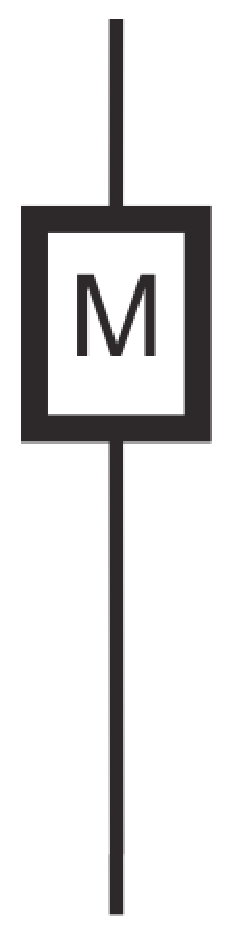
\includegraphics[width=0.63\linewidth]{figures/ddact.pdf}
    \caption{DD}
    \label{fig:dd}
  \end{subfigure}
  \begin{subfigure}{.15\textwidth}
    %\centering
    
\includegraphics[width=0.63\linewidth]{figures/SEAact.pdf}
    \caption{SEA}
    \label{fig:sea}
  \end{subfigure}
  \begin{subfigure}{.15\textwidth}
    %\centering
    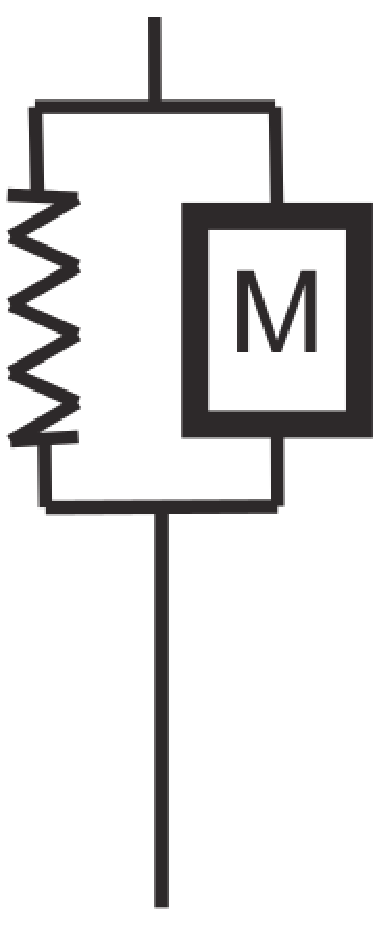
\includegraphics[width=\linewidth]{figures/PEAact.pdf}
    \caption{PEA}
    \label{fig:pea}
  \end{subfigure}
  \begin{subfigure}{.15\textwidth}
    %\centering
    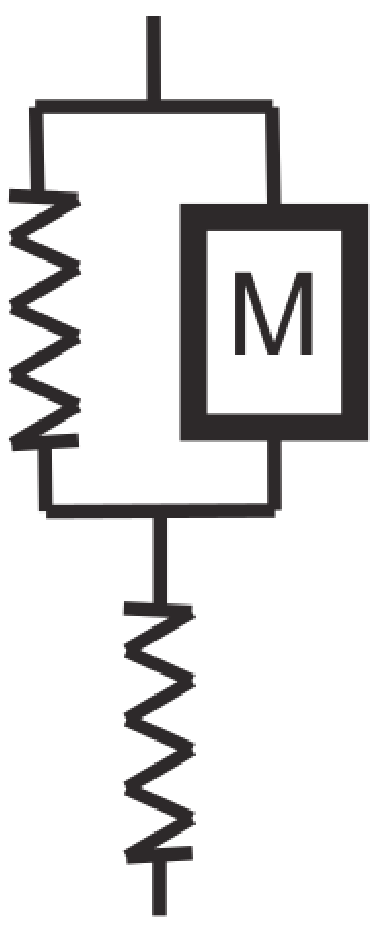
\includegraphics[width=\linewidth]{figures/SEA+PEAact.pdf}
    \caption{SEA+PEA}
    \label{fig:sea_pea}
  \end{subfigure}
  \caption{Four configurations for elastic actuators as from \cite{grimmer}}
  \label{fig:pasive_actuators}
\end{figure}  


%Flexible vs stiff drive train
%Power peak and average consumption comparisons --> energy storage 
%Protection against impact forces on landing phase
% subsubsection elastic_actuator_configuration (end)

\subsubsection{Compliance distribution and implementation} % (fold)
\label{ssub:compliance_distribution_and_possible_configurations}
The results in \cite{grimmer} demonstrate that the implementation of compliance in any of its variants in knees and ankles, influences notably the peak power and energy requirements both for walking and running.
They also seem to prove that the contribution to the reduction of energy consumption and power requirements of the hip is neglectable.
These findings have been used to justify the implementation of elastic actuators in knees and ankles, but not in the hip joints, actuated through direct transmission.

Several models from literature have been subject to a comparative analysis for their use in RuBi, being the main ones shown in Figure \ref{fig:compliance_series} and \ref{fig:compliance_parallel} for the ankle actuation (equivalent for the knees).
These schematics depict the three major design choices made so far, summarized in \ref{list:design_criterias}.
A short summary of the conclusions reached by these studies is introduced below.

\begin{itemize}
\label{list:design_criterias}
  \item Reduction of limbs inertias by placing the actuators up on the links.
  \item Use of transmission to solve the transfer of power motor-joint.
  \item Introduction of compliance through the use of springs.
\end{itemize}

\paragraph{SEA 1 and 2} % (fold)
\label{par:sea_1_2}
\ref{fig:series1} depicts an unidirectional SEA that has to be implemented together with a counterpart, which could be a passive spring or another actuator.
In that case the actuator task would only be the retraction of the foot to reduce its angle with respect to the lower leg, while the passive spring function would imitate the calf muscle.
This approach would be closer to the real functioning of the muscles in the legs, as explained in \ref{sec:bipedal_walking_and_running_gaits}.
However this configuration was discarded due to the complexity in the realization of a correct mapping between the angular displacement of the motor pulley and the ankle joint.

The configuration in Figure \ref{fig:series2} was found in \cite{biobiped}.
It solves the problem found for \ref{par:sea_1_2} changing the configuration of the motor and introducing a fixed pulley.
The influence of the relationship between $L_{B}$ and $L_{A}$ in the ratio between motor and joint torques was studies for this configuration in order to find the optimal dimensions.
However, this solution was discarded in favor of the current one, which demonstrated to be simpler to implement.
% paragraph sea_1_2 (end)

\begin{figure}[h]
\centering
  \begin{subfigure}{.19\textwidth}
    \centering
    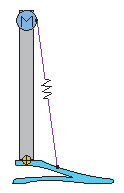
\includegraphics[width=\linewidth]{figures/illustration_serial_direct_i.pdf}
    \caption{SEA 1}
    \label{fig:series1}
  \end{subfigure}
  \begin{subfigure}{.2\textwidth}
    \centering
    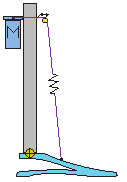
\includegraphics[width=\linewidth]{figures/illustration_serial_pulley.pdf}
    \caption{SEA 2}
    \label{fig:series2}
  \end{subfigure}
  \begin{subfigure}{.19\textwidth}
    \centering
    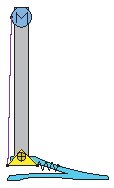
\includegraphics[width=\linewidth]{figures/illustration_serial_direct_ii.pdf}
    \caption{SEA 3}
    \label{fig:series3}
  \end{subfigure}
  \begin{subfigure}{.19\textwidth}
    \centering
    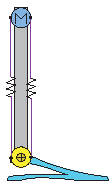
\includegraphics[width=\linewidth]{figures/illustration_serial_elastic_band.pdf}
    \caption{SEA 4}
    \label{fig:series4}
  \end{subfigure}
  \begin{subfigure}{.19\textwidth}
    \centering
    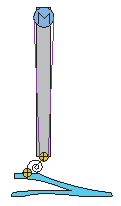
\includegraphics[width=\linewidth]{figures/illustration_serial_rotational.pdf}
    \caption{SEA 5}
    \label{fig:series5}
  \end{subfigure}
  \caption{SEA configurations studied}
  \label{fig:compliance_series}
\end{figure}  

\paragraph{SEA 3} % (fold)
\label{par:sea_3}
The spring configuration in \ref{fig:series3} was found in \cite{grimmer} for a prosthetic ankle design (meaning that the configuration should be adapted for the knee).
It was just used as a study case and source of ideas. 
% paragraph sea_3 (end)

\paragraph{SEA 4} % (fold)
\label{par:sea_4}
The configuration in \ref{fig:series4} was also found in \cite{biobiped} and is known as bidirectional SEA.
It was considered the most optimal to mimic the human musculature on the legs and its implementation through springs attached to the belts or with elastic bands (bungee cords) like the utilized in \cite{imperial_college} was object of analysis.
% paragraph sea_4 (end)

\paragraph{SEA 5} % (fold)
\label{par:sea_5}
The configuration called SEA 5 and shown in Figure \ref{fig:series5} was the selected one.
The original idea was taken from \cite{phides} but has been modified to ease its construction and provide more robustness to the final design.
In \cite{phides} this elastic transmission is implemented with torsion bars for the joints axes, while RuBi uses torsion springs placed around more resistant axis to transmit the motion.
% paragraph sea_5 (end)

\begin{figure}[ht!]
\label{fig:compliance_parallel}
\centering
  \begin{subfigure}{.19\textwidth}
    \centering
    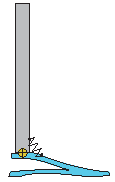
\includegraphics[width=\linewidth]{figures/illustration_parallel_prismatic.pdf}
    \caption{PEA 1}
    \label{fig:parallel1}
  \end{subfigure}
  \begin{subfigure}{.19\textwidth}
    \centering
    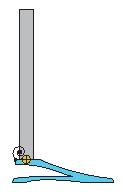
\includegraphics[width=\linewidth]{figures/illustration_parallel_rotational.pdf}
    \caption{PEA 2}
    \label{fig:parallel2}
  \end{subfigure}
  \caption{PEA configurations studied}
\end{figure}  

\paragraph{PEA 1} % (fold)
\label{par:pea_1}
The configuration in \ref{fig:parallel1} shows a compression spring (or extension spring depending the placement) connected within the two links.
This direct connection act as a parallel spring and has the advantage of being a very flexible system in terms of changing the physical parameters of the spring. 
However its design was discarded in favor of the rotational due to the previous election of the rotational series spring.
% paragraph pea_1 (end)

\paragraph{PEA 2} % (fold)
\label{par:pea_2}
The configuration called PEA 2 and shown in Figure \ref{fig:parallel2} was the selected one.
This is congruent with the series spring what will facilitate its integration when designing.
It also has the advantage of having common interfaces which would lead to the possibility of using the same springs for series and parallel configurations, saving thus money and time.

% paragraph pea_2 (end)


% Based on the experiments carried out in \cite{grimmer}, can be deduced that both PEA and SEA configurations have the advantages of reduce the peak and energy requirements of the motors.
% This causes a general improvement of the system due to if smaller motors are needed, the robot will be lighter and thus the structure of the link will weight less too.
% When comparing both configurations though, it is not exactly clear what are the benefices and the pitfalls of SEA, PEA and SEA+PEA.
% This is why a system that allows to have all the configurations is decided which would let the user to choose and implement its own configurations (SEA, PEA or SEA+PEA) and study their behaviors along with the controllers.
\todo{a paragraph has been commented. check if useful or not. i dont think so}
% subsubsection compliance_distribution_and_possible_configurations (end)

% subsection compliance (end)

% section joints (end)

% chapter analysis (end)
    %!TEX root = ../../report.tex
\chapter{Mathematical model of RuBi} % (fold)
\label{cha:mathematical_model}

The motivation to start the development of the mathematical model was the seek of a set of equations with which calculating the requirements for the actuators could be easily achievable.
This task finally evolved towards the construction of a simple dynamic model of the robot and the formulation of the vertical jump dynamics case.
The main goal was to compute the values of the necessary parameters to select joint actuators able to keep up with the requirements of the application.
However, by definition, to do so the application needed to be defined to the extent that these dimensions could be obtained.
Thus, this chapter contains the definition of the task RuBi is expected to be able to perform, the control model defined for it and an explanation of the assumptions made in order to simplify the resulting model. 
After, the necessary kinematic model of the robot is presented as an intermediary step to compute the simplified dynamic model of the robot, which is introduced next to it.
All the algorithms described in this chapter have been implemented in MATLAB and the scripts can be found in the source folder attached to this report.

%!TEX root= ../../../report.tex

\section{Actuators design}
\label{sec_actuators}
The following sections present the calculations carried out to define the load requirements of the application the actuators will be used for\footnote{For an introduction to the actual hardware implemented in the prototype, the user is referred to section \ref{sec:electronics}}.
In the present case, the operation consists in the generation of walking and running gaits for the planar robot RuBi at a wide, not-specified range of speeds. 
Due to the complexity of modeling such wide and uncertain task requirements, it was decided to study the case of the robot hopping on one leg assuming that the drive requirements for walking/running would be accomplished by actuators able to perform this action.

Considerations about the mechanical transformations of the motor output power before being driven to the load such as transmission mechanisms are not detailed here, but in \ref{sub:pulleys_and_belts}.
The present explanations are for the motor and gearbox selection.

Following feasibility and availability criteria, it was decided to utilize electric motors for the construction of the robot, as in many other similar cases in the literature like \cite{runbot1}, \cite{phides} or \cite{biobiped}.
Generally, the process of selection of electric motors entails answering the following queries about the load:

\begin{itemize}
\label{list:motor_selection}
	\item Torques applied by the load to the motor shaft for every link $\tau_{i}$.
	\item Accelerations involved $\ddot{q_{i}}$.
	\item Inertias of the masses $I_{i}$.
	%\item Maximum voltage and current supply available 
	\item Type of operation (continuous, intermittent, reversing).
	\item Actuator size constraints.
\end{itemize}

The first three points in \ref{list:motor_selection} have been answered in sections \ref{sec:jumping_case}, \ref{sec_kinematic_model} and \ref{sec_dynamic_model}.
%Move next paragraph to electronics section?
The expected experiments for RuBi to be used are not meant to be of a long duration, which means that low numbers of cycles are expected per use corresponding to an intermittent application.
Besides, as explained in the power requirements sections of \cite{grimmer} Manuscript I, high power peaks per cycle specially in knees and ankles are expected.
For the above reason, and aiming at constructing as further work an on-board electronics set, batteries LiPo of 6 cells and 0.85A have been selected to supply the necessary power to the motors.
Finally, the physical dimensions of the motors such as weight and volume are a key factor to be consider in the design of moving platforms. 
Naturally, the aim here has always been to find a motor+gearbox combination to keep the overall weight of the robot as low as possible, since it was assumed that it would be the heaviest part in the structure.

%!TEX root = ../../../report.tex

\section{Analysis of vertical jump} % (fold)
\label{sec:jumping_case}
Modeling the dynamics of walking gaits in a bipedal robot with 6 DOF has proved significantly complex and time consuming, even for the two-dimensional case.
However, it is essential for the obtainment of the most extreme torque and rotational velocity values to apply to each joint during the motion, necessary to gauge the required actuators for the application.
In order to ease the task, instead of calculating the motion equations for the walking or running cases, it was resolved to model the dynamics of the vertical jump case.
This was decided under the assumption that a platform able to perform a static, vertical jump of a certain height $h$ and determined characteristics on one leg could be able to fulfill the power requirements necessary for running, both from an actuation and a structural point of view.
This assumption was built upon the findings introduced in \cite{jump-run1} and \cite{jump-run2}.

\subsubsection{Vertical jump dynamics} % (fold)
\label{ssub:static_jumping_dynamics}
As explained in section \ref{sec:dimensions}, the dimensions of the robot and its parameters have been conceived to imitate human characteristics and capabilities.
Therefore the jump analysis here will be carried out in resemblance of the human case, based on \cite{jump-dynamics1} and aiming at applying the results to a robot platform, as in \cite{jump-dynamics2}.
The jump case analyzed here can be described according to \cite{jump-dynamics1} as a static, squat jump over one foot with take-off and without counter-movement (SJ-NAS).
Three assumptions have been made regarding the bodies in contact during the landing phase of the robot as listed in \ref{list:assumptions_jump}.

\begin{itemize}
\label{list:assumptions_jump}
    \item No slipping occurs.
    \item Absence rebounding.
    \item There are no structural deformations.
\end{itemize}

The whole jump cycle has been divided into two phases with different analysis: an impulse and an aerial period.
\begin{figure}[ht!]
    \centering
    \begin{subfigure}[b]{0.3\textwidth}
        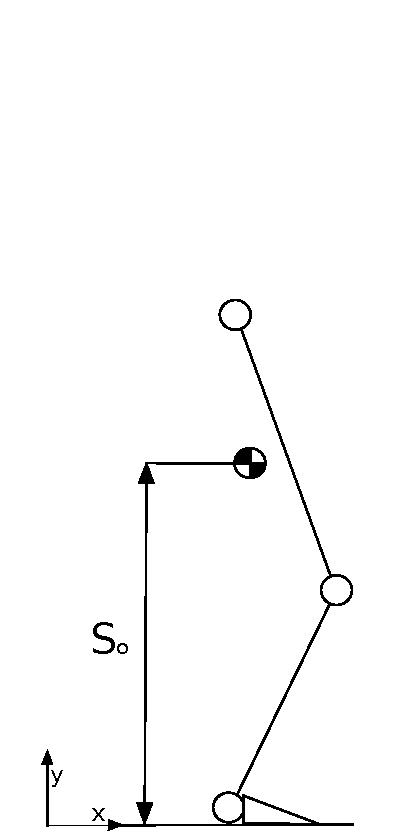
\includegraphics[width=\textwidth]{figures/launch_phase.pdf}
        \caption{Launch phase}
        \label{fig:launch_phase}
    \end{subfigure}
    \begin{subfigure}[b]{0.3\textwidth}
        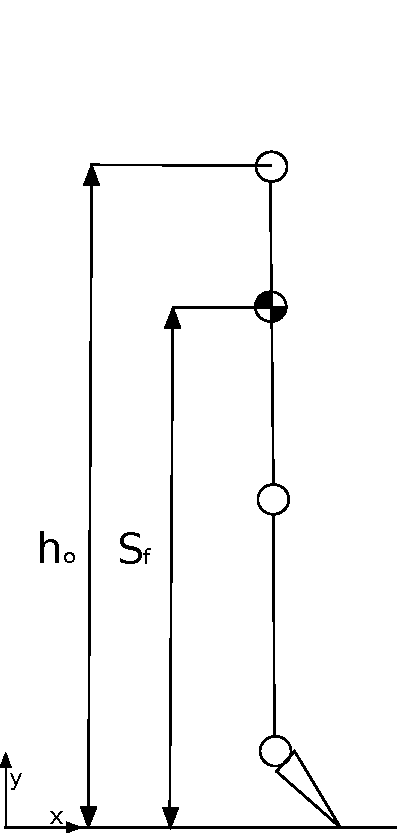
\includegraphics[width=\textwidth]{figures/takeoff_phase.pdf}
        \caption{Takeoff phase}
        \label{fig:takeoff_phase}
    \end{subfigure}
    \begin{subfigure}[b]{0.3\textwidth}
        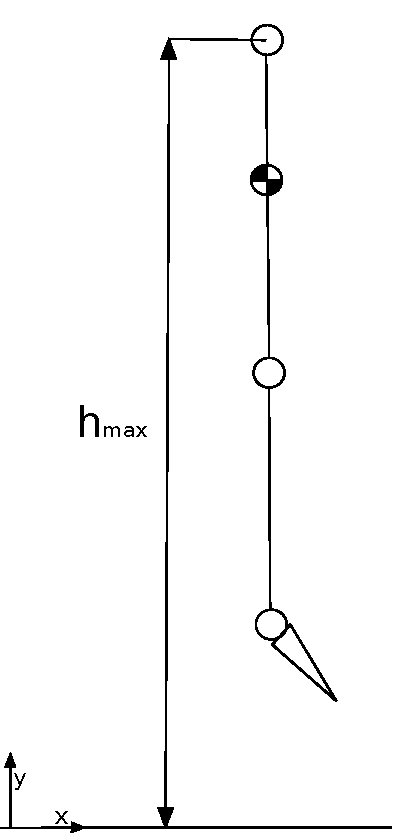
\includegraphics[width=\textwidth]{figures/flight_phase.pdf}
        \caption{Aerial phase}
        \label{fig:aerial_phase}
    \end{subfigure}
    \caption{Jump phases without fall and landing.}
    \label{fig:jump_phases}
\end{figure}
\paragraph{The aerial phase}
The period from the take-off of the toes to the instant in which the maximum height $h_{max}$ has been reached, which takes place between the instants represented in \ref{fig:takeoff_phase} and \ref{fig:aerial_phase}. 
The rest of the cycle, including fall and landing are not described here.
During the whole period the robot is considered a rigid solid.
This phase is analyzed following the equations of a static projectile motion for the vertical launch case, expressed in \ref{eq:vertical_motion} and \ref{eq:vertical_energy}.
\begin{equation}
\label{eq:vertical_motion}	
	h(t) = V_o t sin(\theta) - \cfrac{1}{2} g t^2 
\end{equation}

\begin{equation}
\label{eq:vertical_energy}
	m g \Delta h = \cfrac{1}{2} m \Delta V^2
\end{equation}
The equation \ref{eq:vertical_energy} is an energy balance analysis for the flight phase, that can be rearranged as showed in \ref{eq:deltaV}
\begin{equation}
\label{eq:deltaV}
	\Delta V = \sqrt{2 g \Delta h}
\end{equation}
This equation can be used to input the desired displacement in the CoG of the robot during the free flight period and obtain the necessary velocity at take-off $V_{toff}$, which is the one the robot has to reach in the impulse phase.
This can be done since $V_{final} = 0$ and therefore $\Delta V = V_{toff}$.

\paragraph{The impulse phase}
From the initial position at the beginning of the jump, depicted in \ref{fig:launch_phase}, to the instant when the toes of the standing foot take off the ground and the ground reaction force ceases, shown in \ref{fig:takeoff_phase}.
The change in momentum in the robot, of total mass $m$, caused by the application of a vertical force with the foot to the ground $F$ during a period $t$ is given by equation \ref{eq:impulse}, derived from the second law of motion of Newton.
\begin{equation}
\label{eq:impulse}
	F  t = m  \Delta V	
\end{equation} 
Substituting equation \ref{eq:deltaV} in \ref{eq:impulse}, the necessary impulse to reach the desired maximum height can be computed.
However, since the force applied to the mass and the application period cannot be decoupled from the result of the equation, an energy analysis has to be carried out together with a posterior optimization of the two values for the desired design of the robot.
Solving equation \ref{eq:impulse} for a small range of application time values and after computing \ref{eq:deltaV} with increasing values of $\Delta h$ in the range $[0.01,0.1]$ meters yields a reciprocal graph whose positive quadrant can be seen in Figure \ref{fig:f-t}
\begin{figure}[ht!]
	\centering
	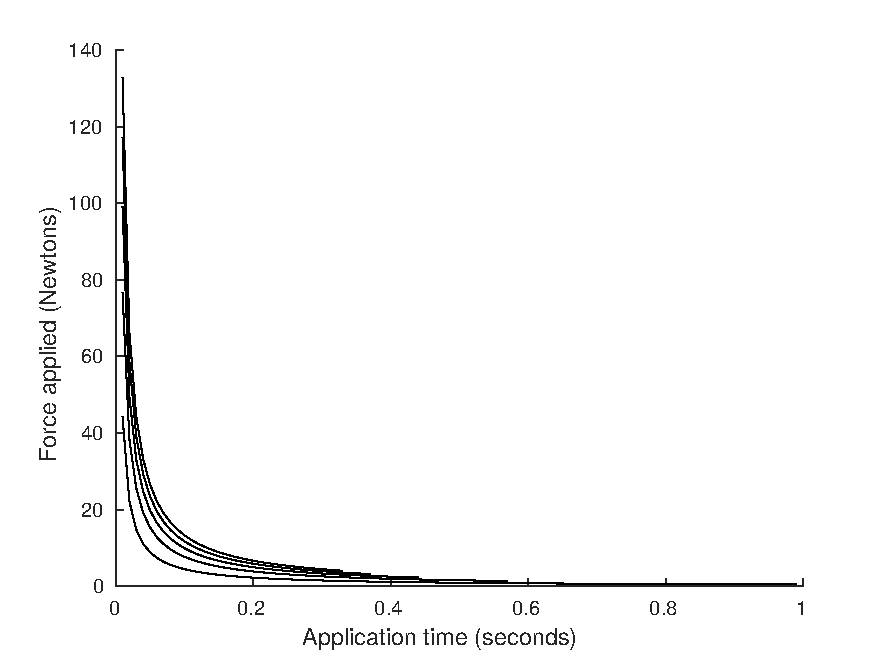
\includegraphics[width=0.8\textwidth]{figures/force-timePlot.pdf}
	\caption{Force-application time values for the same work magnitude.}
	\label{fig:f-t}
\end{figure}
However, the obtained graphs do not propagate to an infinite value of application time, existing a boundary farther than which, the impulse will not produce enough variation in the momentum to launch the body.
\begin{equation}
\label{eq:work}
	W = \int_{t_{toff}}^{t_{f}} F(t)\,\mathrm{d}t = \cfrac{1}{2} m \Delta V^2 = F_{min} S
\end{equation}

Equation \ref{eq:work} describes how the work performed by the robot during the impulse phase can relate to the change in its kinetics energy. 
This equation, derived also from Newton's second law would only apply to rigid bodies without internal degrees of freedom, which is not the case.
However, it has been assumed that the displacement given by $S$ is the vertical translation of the CoM of the robot during the impulse and that it is small enough to be a valid assumption in order to use this procedure.
From Figure \ref{fig:jump_phases}, the displacement of the CoM during the impulse is given as $S=S_{f}-S_{o}$.
Knowing the value of $S$, the minimum necessary force can be obtained, and hence its corresponding application time on Figure \ref{fig:f-t} for a given $\Delta h$.
The displacement of the CoM, $S$ will depend on the initial configuration of the robot prior starting the impulse, and its final one.
Furthermore, for a given $\Delta h$, a range of possible values of the ground reaction Force $F$ can be computed within the limits established and a time can be obtained.
Thus, for a determined $\Delta h$ and $t$ values, a $F$ has to be applied by the foot again the ground.
In order to translate that force to joint effort, the dynamic model of the robot is required.

% subsubsection static_jumping_dynamics (end)

% section The_jumping_case (end)
%!TEX root= ../../../report.tex

\section{Kinematic model}
\label{sec_kinematic_model}
The kinematics model of the robot describes the motion of every joint in time disregarding dynamic parameters.
It is used here to compute position, velocity and acceleration of the limbs for given trajectories of the toes, which are the contact point with the ground in the presented study case, through their forward kinematics.
Also the inverse kinematic model is constructed as a tool for the posterior computation of the dynamics model and its application to model the necessary actuators.
The model has been obtained through direct application of trigonometry instead of using the D-H parameters given its simplicity.
To do so, as explained before the case has been reduced to a two-dimensional study of one leg, where each robot leg has been analyzed as a kinematic chain of three degrees of freedom.
The main reference frame has been placed attached to the hip with its Y axis parallel to the ground, as if this was the base of a robotic arm, and the toe was the tool, has shown in Figure \ref{fig:kinematics}.
This representation has been chosen to ease the construction of the mathematical model.
\todo{add world reference frame attached to the ground for flight phase study}
\begin{figure}[ht]
	\centering
	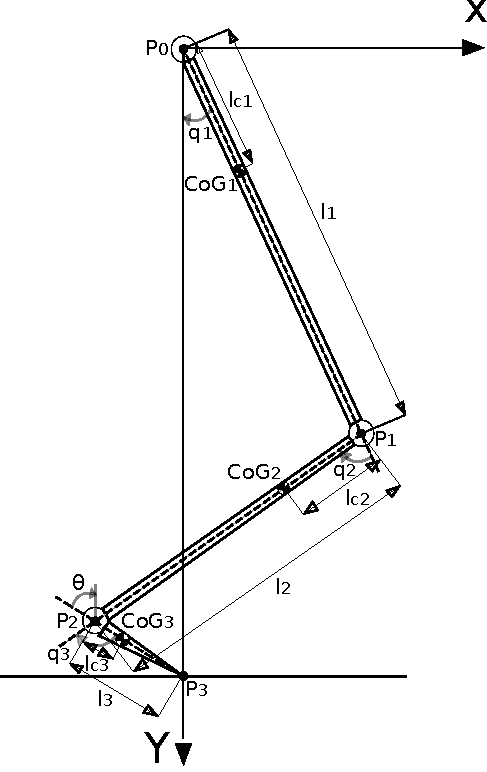
\includegraphics[width=0.4\textwidth]{figures/kinematics_model.pdf}
	\caption{Coordinate definitions for the schematic model of one leg}
	\label{fig:kinematics}
\end{figure}
\todo{Add ground reference frame}

The Figure \ref{fig:kinematics} depicts the schematic representation of only one leg, since the other one is equivalent. 
The system is said to be in single support phase since there would be just one foot in contact to the ground.
In the analyzed case, the swinging leg (not represented in Figure \ref{fig:kinematics}) would be static and could be considered an additional link with no degrees of freedom.
The variables $q_{i}$ represent the angles of the joints with respect to their fully-stretched positions to simplify the obtainment of the forward kinematic model, while the angle $\Theta$ is used to express the orientation of the ankle in an absolute manner. 
From Figure \ref{fig:kinematics}, the forward kinematic model in \ref{eq:forward_kinematics} can be easily obtained.
\begin{equation}
\label{eq:forward_kinematics}
	\begin{aligned}
		x_{0} &= 0 \\
		y_{0} &= 0 \\
		x_{1} &= l_{1} \sin(q_{1}) \\
		y_{1} &= l_{1} \cos(q_{1}) \\
		x_{2} &= l_{1} \sin(q_{1}) + l_{2} \sin(q_{1}+q_{2}) \\
		y_{2} &= l_{1} \cos(q_{1}) + l_{2} \cos(q_{1}+q_{2}) \\
		x_{3} &= l_{1} \sin(q_{1}) + l_{2} \sin(q_{1}+q_{2}) + l_{3} \sin(q_{1}+q_{2}+q_{3}) \\
		y_{3} &= l_{1} \cos(q_{1}) + l_{2} \cos(q_{1}+q_{2}) + l_{3} \cos(q_{1}+q_{2}+q_{3}) 
	\end{aligned}
\end{equation}
The variables $x_{i}, y_{i}$ represent the position coordinates of the joints in the right leg, named $P_{i}$ in the schematic in Figure \ref{fig:kinematics} and $P'_{i}$ for the left leg (not depicted).
Once computed, the linear velocity and acceleration of every joint can be obtained by derivation of the forward kinematic model and represented as $\dot{P}_{i}$ and $\ddot{P}_{i}$.

\todo{Add space state vector}
The model presented is the most basic one and does not contain the degrees of freedom that could be introduced by springs in the actuators.
This is due to two reasons:
\begin{itemize}
	\item Their configuration can be changed to series, parallel or none in both knees and ankles.
	\item The study of the jump case regarding the parameterization of the actuators has been carried out in the most disadvantageous scenario from the energetic point of view, which in this case means no springs.
\end{itemize}

Following the same approach, the inverse kinematic model can be computed for the right leg, yielding the equations \ref{eq:inverse_kinematics}.
\begin{equation}
\label{eq:inverse_kinematics}
	\begin{aligned}
		x_{2} &= x_{3} - l_{3} \sin(\Theta) \\
		y_{2} &= y_{3} - l_{3} \cos(\Theta) \\
		q_{1} &= \arctan \left(\frac{x_{2}}{y_{2}}\right) - \arccos \left(\frac{x_{2}^2 + y_{2}^2 + l_{1}^2 - l_{2}^2}{2 l_{1} \sqrt{x_{2}^2 + y_{2}^2}}\right) \\
		q_{2} &= \pi - \arccos \left(\frac{l_{1}^2 + l_{2}^2 - x_{2} - y_{2}}{2 l_{1} l_{2}}\right) \\
		q_{3} &= \Theta - q_{1} - q_{2} \\
	\end{aligned}
\end{equation}
And equivalently to the forward kinematics, the inverse kinematic model can be derived to obtain the velocities and accelerations in the joint space $\dot{q_{i}}$ and $\ddot{q_{i}}$.

%!TEX root= ../../../report.tex
\section{Dynamic model}
\label{sec_dynamic_model}
The goal of this step is to calculate the relationship between an external force applied to the toe (ground reaction force while jumping) and the necessary torques in the joints for dealing with that external disruption.
This relation can be expressed as a set of second order differential equations represented for the general case as in equation \ref{eq:dynamics_eq1}. 
\begin{equation}
	\label{eq:dynamics_eq1}
	B(q)\ddot{q} + C(q,\dot{q})\dot{q} + g(q) = \tau
\end{equation}
Where $B(q)$ is the inertia matrix, $c(q,\dot{q})$ contains the centrifugal and coriolis acceleration terms and $g(q)$ represents gravity, as in \cite{dynamics1} and \cite{dynamics2}. 
It must be remarked here that the constructed model does not introduce joint friction terms.
For an open kinematic chain as this, three methodologies to obtain the above equation where object of study:
\begin{itemize}
	\item A simplified Euler-Lagrange algorithm, as introduced in \cite{E-L1}, which makes use of the Lagrangian formulation to describe the behavior of the system through work and energy.
	\item The so called Energy Method, presented in \cite{asada} and consisting in finding the relation between the force in the end-effector and the joint torques through the Jacobian of the kinematic chain.
	\item The Newton-Euler algorithm, through which the dynamics of the system can be expressed in terms of forces and moments applied in each member of the chain.
\end{itemize}
It was finally decided to apply the third option due to the fact that it was faster to implement than the E-L algorithm and more reliable than the Energy method.
The Newton-Euler algorithm is founded in classical mechanics and its a recursive method that computes in two steps the velocities and accelerations of every component of a kinematic chain and their forces and torques on the joints.
In \ref{eq:N-E_eq1}, the equations of motion for an individual link are shown.
\begin{equation}
\label{eq:N-E_eq1}
	\begin{aligned}
		f_{i-1, i} - f_{i,i+1} + m_{i} g - m{i} \dot{V}_{ci} =& 0 \\
		N_{i - 1 , i} - N_{i , i + 1} - ( r_{i - 1 , i} + r_{i , Ci} ) \times f_{i - 1 , i} + ( - r_{i , Ci} ) \times ( - f_{i , i + 1}) - I_{i} \dot{\omega_{i}} - \omega_{i} \times ( I_{i} \omega_{i} ) =& 0 \\
		i = 1,..., N 
	\end{aligned}
\end{equation}
These equations contain the coupling forces and moments applied to the link by the immediate ones, however, they cannot be used with them. 
$\omega_{i}$ and $\dot{\omega_{i}}$ represent respectively the angular velocity and acceleration vectors of link $i$ and can be obtained from the joint velocities and accelerations, computed in the previous section, as in equation \ref{eq:angular_magnitudes}.
$I_{i}$ are the inertia matrices of the links, calculated in SolidWorks for the final design of RuBi.
\begin{equation}
\label{eq:angular_magnitudes}	
	\begin{aligned}
		\omega_{i} &= \omega_{i-1} + \xi_{i}\dot{q}_{i}Z_{base}^i\\
		\dot{\omega_{i}} &= \dot{\omega_{i-1}} + \xi_{i}[\ddot{q}_{i}Z_{base}^i + \dot{q}_{i}\omega_{i-1} \times Z_{base}^i]
	\end{aligned}
\end{equation}
The closed-form equations must be derived from them so that they can be applied to the algorithm.
This is done by substituting the coupling forces in the final set of 6 equations obtained for $N=3$ and substituting \ref{eq:torques} in the resulting equations.
\begin{equation}
\label{eq:torques}
	N_{i - 1 , i} = \tau_{i}
\end{equation}
Equation \ref{eq:torques} is valid only for the planar case.
After these steps, a set of three equations of the form \ref{eq:dynamics_eq1} is obtained. 
As parameters, they contain the masses of the links, their vectorial positions, the gravity term and their inertia matrices. 

\todo{add final motion equations?}
This set of equations calculates the necessary torques on the joints as a function of the joints displacements and the external forces and torques applied on the system, as represented in \ref{eq:tau_q}.
\begin{equation}
\label{eq:tau_q}
	\tau(t)_{i} = f(q_{i}(t), \dot{q}_{i}(t), \ddot{q}_{i}(t), \tau_{ext}, F_{ext})
\end{equation}
However, in order to use it the functions that model the trajectories of joints in the joint space must be approximated.
For the ideal static, vertical jump case under study here, the movement of the toe has been constrained to a vertical displacement along the $Y$ axis in order to simplify this task.
Thus, the trajectory of the end-effector of the kinematic chain, $P_{3}$ in Figure \ref{fig:f-t}, can be easily approximated as a function of the form shown in 
\begin{equation}
\label{eq:toe_trajectory}
	\begin{aligned}
	x_{3}(t) &= 0 \\
	y_{3}(t) &= y_{3}(t_{o}) + \cfrac{y_{3}(t_{f}) - y_{3}(t_{o})}{(t_{f} - t_{o}) (t - t_{o})} \\
    \theta(t) &= \theta(t_{o}) + \cfrac{\theta(t_{f}) - \theta(t_{o})}{(t_{f} - t_{o}) (t - t_{o})} 
    \end{aligned}
\end{equation}
Therefore, if equation \ref{eq:toe_trajectory} is used as the input to the inverse kinematic model, the joint displacements will become dependent on the linear displacement of $P_{3}$, and equations \ref{eq:tau_q} will be rewritten as \ref{eq:tau_p}.
\begin{equation}
\label{eq:tau_p}
	\tau(t)_{i} = f(P_{3}(t), \tau_{ext}, F_{ext})
\end{equation}
%!TEX root= ../../../report.tex

\section{Springs influence in the actuation}
\label{sec_springs}
This section deals with the calculations carried out in order to model the influence of the implemented compliance in terms of energy efficiency and joint torque requirements.
As explained in \ref{sec:joints}, the selection of the elastic actuators installed and their configuration on RuBi has been left as a customizable feature for research purposes.
This, together with the fact that RuBi has not been designed to optimize a specific type of gait made pointless the calculation of optimal values of springs.
Thus, the following is just a theoretical frame presented to provide an easy method to compute the influence of the springs in the performance once the user has selected them.
It was meant to be used for the experiments devised on compliance influence in hopping motion, presented in \ref{cha:experiments}.

\subsection{Torque and energy contribution of passive actuators} % (fold)
\label{sub:torque_contribution_of_passive_actuators}
All the springs that can be assembled in RuBi are torsional, as explained in \ref{fig:knee_joint}, whose general equations for torque and energy storage are shown in \ref{eq:torsion_spring}. 
\begin{equation}
\label{eq:torsion_spring}
\begin{aligned}
	\tau_{S} &= -K \Delta \theta \\
	U_{S} &= \frac{1}{2}K \Delta \theta^2
\end{aligned}
\end{equation}
The contribution of the springs torques to the system actuation is therefore modeled introducing the torque equation in \ref{eq:torsion_spring} on the right side of \ref{eq:dynamics_eq1}, which would yield equation \ref{eq:dynamics_eq2}.
Where the torques vector has been divided into the motors and springs inputs.
\begin{equation}
	\label{eq:dynamics_eq2}
	B(q)\ddot{q} + C(q,\dot{q})\dot{q} + g(q) = \tau_{M} + \tau_{S}
\end{equation}
The values of $\Delta \theta_{i}$ (where i=1,..,N denotes the joint index) can be obtained through forward kinematics for given trajectories, while $\tau_{i}$ can be computed from equation \ref{eq:dynamics_eq1} given the ground contact force model, which is the only external force applied to the system.
Thus, the first formula in \ref{eq:torsion_spring} can be used to calculate the optimal $K$ for a desired joint trajectory and force model, for instance.
Knowing $k_{i}$ and $\Delta \theta_{i}$, the energy stored per gait cycle by each spring can be computed and utilized for studying their influence on the performance of the robot.

\subsection{Joint kinetics} % (fold)
\label{sec:joint_kinetics}
The formulas presented in this section have not utilized during this project. 
They are mainly introduced here as a part of the theoretical frame provided to ease the use of the RuBi robot in energy studies for locomotion.
It use was planned as a part of the experiments devised in the influence of the compliance configuration in energy storage.

The motor power requirements for each joint can be calculated through equation \ref{eq:motor_power} for direct drive transmission.
This formula does not include inertias, frictions or any other efficiency coefficients. 
\begin{equation}
\label{eq:motor_power}
	P_{m} = \dot{\theta}_{m} \tau_{m}
\end{equation}
By definition of \ref{eq:motor_power}, the value of $P_{m}$ can be positive (motor thrusting) or negative (motor dumping).
Thus, the peak power in the motion cycle can be computed as the its maximum absolute value.
Besides, the equation of motor power is used in \ref{eq:energy_requirement} for calculating the overall energy requirements for a whole motion cycle, employing only absolute values as well.
\begin{equation}
\label{eq:energy_requirement}
 	E_{cycle} = \int{P_{m+}(t) dt} + \int{P_{m-}(t) dt}
 \end{equation} 

\subsubsection{Influence of elastic actuation} % (fold)
\label{sub:influence_of_elastic_actuation}
The above presented are general formulations.
However, the introduction of elastic transmission between motor and load through springs modify the computation of motor power.
The changes resulting from implementing the configurations shown in Figure \ref{fig:sea}, \ref{fig:pea} and \ref{fig:sea_pea} yield equations \ref{eq:SEA_power}, \ref{eq:PEA_power} and \ref{eq:SEA_PEA_power} respectively, as per \cite{grimmer}.
These equations model the conjunction of the torques provided by the motor and the springs, this one defined by their stiffness constants and the angle they are bent.
For a complete and detailed description of the parameters in these equations, the reader is referred to the cited paper.
\begin{equation}
\label{eq:SEA_power}
	P_{m} = \tau_{m} \left(\dot{\theta}_{t} + \frac{\dot{M}_{ex}}{K_{s}}\right)
\end{equation}

\begin{equation}
\label{eq:PEA_power}
	P_{m} = (F_{ex} + (K_{p} \Delta \theta_{t})) \dot{\theta}_{t}
\end{equation}

\begin{equation}
\label{eq:SEA_PEA_power}
	P_{m} = \left(F_{ex} + (K_{p} \Delta \theta_{m}) \left(\theta_{t} + \frac{\dot{F}_{ex}}{K_{s}}\right)\right)
\end{equation}

% subsubsection influence_of_elastic_actuation (end)

% section joint_kinetics (end)
% %!TEX root= ../../../report.tex

% \section{Joint kinetics} % (fold)
% \label{sec:joint_kinetics}
% The motor power requirements for each joint can be calculated through equation \ref{eq:motor_power} for direct drive transmission.
% This formula does not include inertias, frictions or any other efficiency coefficients. 

% \begin{equation}
% \label{eq:motor_power}
% 	P_{m} = \dot{\theta}_{m} \tau_{m}
% \end{equation}

% By definition of \ref{eq:motor_power}, the value of $P_{m}$ can be positive (motor thrusting) or negative (motor dumping).
% Thus, the peak power in the motion cycle can be computed as the its maximum absolute value.
% Besides, the equation of motor power is used in \ref{eq:energy_requirement} for calculating the energy requirements for a whole motion cycle, employing only absolute values as well.

% \begin{equation}
% \label{eq:energy_requirement}
%  	E_{cycle} = \int{P_{m+}(t) dt} + \int{P_{m-}(t) dt}
%  \end{equation} 

% \subsection{Influence of elastic actuation} % (fold)
% \label{sub:influence_of_elastic_actuation}
% The above presented are general formulations.
% However, the introduction of elastic transmission between motor and load through springs modify the computation of motor power.
% The changes resulting from implementing the configurations shown in Figure \ref{fig:sea}, \ref{fig:pea} and \ref{fig:sea_pea} yield equations \ref{eq:SEA_power}, \ref{eq:PEA_power} and \ref{eq:SEA_PEA_power} respectively, as per \cite{grimmer}.
% For a complete and detailed description of the parameters in these equations, the reader is referred to the cited paper.

% \begin{equation}
% \label{eq:SEA_power}
% 	P_{m} = \tau_{m} \left(\dot{\theta}_{t} + \frac{\dot{M}_{ex}}{K_{s}}\right)
% \end{equation}

% \begin{equation}
% \label{eq:PEA_power}
% 	P_{m} = (F_{ex} + (K_{p} \Delta \theta_{t})) \dot{\theta}_{t}
% \end{equation}

% \begin{equation}
% \label{eq:SEA_PEA_power}
% 	P_{m} = \left(F_{ex} + (K_{p} \Delta \theta_{m}) \left(\theta_{t} + \frac{\dot{F}_{ex}}{K_{s}}\right)\right)
% \end{equation}

% subsection influence_of_elastic_actuation (end)

% section joint_kinetics (end)
%!TEX root= ../../../report.tex

\section{Model-based controllers}
\label{sec_dynamic_controller}
As introduced in the previous sections, the equations of motion derived for RuBi can be used to compute the necessary output values of its actuators in order to perform an input toes trajectory and external forces, as expressed in \ref{eq:tau_p}.
By definition, this could be sufficient to, appropriately used, be utilized as the base of a controller for the robot, without accounting the own dynamics of the actuators.
As an example of the above said, and despite the early stage in its development in which this model is left, some data has been computed and plotted for proving the concept.
The only trajectory planner current implemented computes vertical straight paths for the toes.
However, more complex trajectory equations could be used to achieve different locomotion patterns.

\begin{figure}[h]
	\centering
	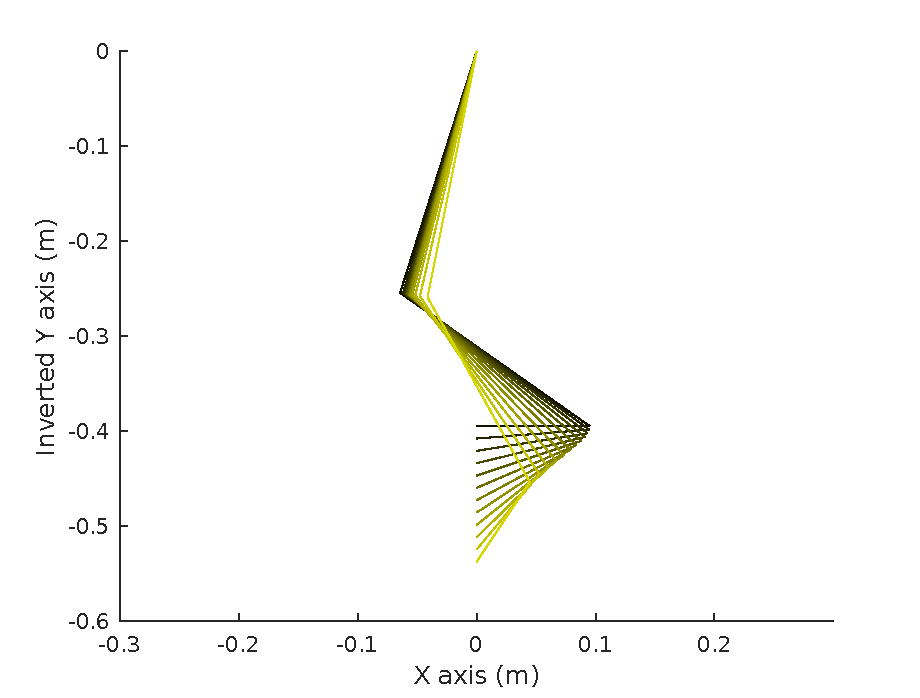
\includegraphics[width=0.5\textwidth]{figures/kinematics_sim.pdf}
	\caption{Joints trajectories from kinematics model}
	\label{fig:controller_position}
\end{figure}

An initial and final toes position has been inputed to \ref{eq:toe_trajectory} to define an example trajectory for the toes in one leg, together with a random value for $\Delta h$.
The output of the kinematics computed for $i=1,...,N$ steps is shown in Figure \ref{fig:controller_position}, where it has been rearranged for visualization.
It can be seen that the toes trajectory does not cover the full range of a vertical jump.

\begin{equation}
\label{eq:joint_vel}
	\dot{\theta}_{i,j} =\frac{ \abs{ \theta_{j}(t_{i}) - \theta_{j}(t_{i-1}) } }{ t_{step} }
\end{equation}

For the trajectory described and $\Delta h$, the impulse equation in \ref{eq:impulse} has been computed and the values $(F_{min}, t_{max})$ from \ref{eq:work} have been used as input to the dynamic model.
The result of computing \ref{eq:dynamics_eq1} for the same time steps is shown in \ref{fig:controller_torque}, together with the solution for equation \ref{eq:joint_vel} in \ref{fig:controller_speed}, calculated in an analogue way.

\begin{figure}[h]
    \centering
    \begin{subfigure}{0.49\textwidth}
        \includegraphics[width=\textwidth]{figures/torque-time.pdf}
		\caption{Joints torque as a function of time}
		\label{fig:controller_torque}
	\end{subfigure}	
    \begin{subfigure}{0.49\textwidth}
        \includegraphics[width=\textwidth]{figures/speed-time.pdf}
		\caption{Joints velocity as a function of time}
		\label{fig:controller_speed}
    \end{subfigure}
\end{figure}

The ranges in which the results in \ref{fig:controller_torque} and \ref{fig:controller_speed} are found seem consistent with the obtained during the experiments detailed in \ref{sub:suitability_of_the_motor_model_for_the_application}.
However, the analysis of their accuracy would entail a more precise construction of the mathematical model and study of kinematic chains dynamics which laid out of the scope of this project since it was not considered a priority goal.


% chapter kinematic_and_dynamic_model (end)
    %!TEX root = ../../report.tex
\chapter{Mechatronic design} % (fold)
\label{cha:design}
The results of the conceptual studies conducted in chapter \ref{cha:analysis} laid the goals and criteria to lead the design process of the first prototype of RuBi.
The actual implementation of these ideas in the fields of electronics, mechanics and software is described here.
When designing from a holistic point of view, these three areas combined give a positive synergy which is the burden of this chapter.
The first of the three sections starts with the design of the electronic hardware: from the selection of the motors based on \ref{sec:joints} and \ref{cha:mathematical_model} to the expansion interfaces installed in order to reduce the weight and finally the sensory feedback system.
It follows the mechanical design of the limbs components, in which the constraints defined in \ref{sec:dimensions} and \ref{sec:physical_properties} are applied, together with the structural and production-oriented calculations required.
It concludes with a presentation of the CAD design process carried out, in which a comprise between the components ideal capabilities and the current production capacity in this project has been tried to be reached.
In the last section, devoted to the software-related development except for the simulation environment, the architecture implemented for the robot control system is presented.

%!TEX root = ../../../report.tex
\section{Electronics} % (fold)
\label{sec:electronics}

%!TEX root = ../../../../report.tex

\subsection{The electric actuators} % (fold)
\label{sub:electric_actuators}
In chapter \ref{cha:mathematical_model}, the necessary characteristics of the actuators have been calculated.
In this section, the resulting theoretical requirements are used to select the final motor $+$ gearbox combination utilized.
All the documentation regarding the control of the actuators software-wise is to be found in section \ref{sec:software}.

\subsubsection{Flat BLDC Maxon motors} % (fold)
\label{ssub:the_bldc_motors}
It must be mentioned at this point that the actuators and their interface were assumed at the beginning of the project to be a very hard constraint in the design from an economic point of view. 
This means that the conception of the robot structure has been influenced by this criteria towards the adaption of the final prototype characteristics (such as final size or mass) to the application range of the available motors at our disposal.
This fact has converted the design in an iterative process of optimization whose final result is a robot that matches the available actuators and not the other way around, as it should be in theory.
In the view of the this, the brushless DC motor $+$ gearbox present in the Locokit robot construction kit, introduced in \cite{locokit} are used in the RuBi prototype.

The flat motors model is 339260 from Maxon motor, whose datasheet can be found in \cite{maxon_motor}, and the planetary gearhead is the number 143976 in datasheet \cite{maxon_gear}.
The electromechanical constants of the motors, together with its nominal supply values or the output power and torque of both the motor and the gearbox can be found in these documents. 
However, the electronics of the motors are designed to constantly overdrive them at $24V$, which has been taken into account when calculating their output.
Furthermore, each motor counts three hall effect sensors able to provide accurate relative position measurements.
% subsubsection the_bldc_motors (end)


\subsubsection{BLDC motor boards} % (fold)
\label{ssub:bldc_motor_boards}
Each BLDC motor in the Locokit comes with a motor board able to control it, designed for 24V and 48W.
They consist of a 48MHz ARM7 processor for time critical control and motor commutation, as stated in \cite{locokit-electronics}, together with 4 general purpose I/O inputs for local sensor interface.
Furthermore, they have two available 8-pin interfaces for the motors, one of them with a standard flex connector used in most of Maxon flat motors.

% subsubsection bldc_motor_boards (end)

\subsubsection{Extension PCBs} % (fold)
\label{ssub:extension_pcbs}
Following the idea of reducing weight and inertias in the structure as explained in chapter \ref{cha:analysis}, it was decided to place all the electronics off-board.
In order to extend the existing motor flex interfaces, a simple extension PCB was manufactured for each device.
The boards have been designed with Eagle following the requirements of current when sizing the width of the paths given by the supplier.
The design lacks of vias which reduces the complexity and facilitates the manufacturing.
The board for the left leg, whose schematic can be seen in \ref{fig:pcb1}\footnote{For the right leg the schematic has been mirrored}, contains a flex connector, like the one originally found on the motor boards, mapped to an 8-pin Molex connector where the wiring to the BLDC board is connected.

\begin{figure}[ht]
	\centering
	\includegraphics[width=0.5\textwidth]{figures/expansion_board.pdf}
	\caption{Left leg extension PCB schematic.}
	\label{fig:pcb1}
\end{figure}

% subsubsection extension_pcbs (end)


% subsection electric_actuators (end)
\subsection{Suitability of the motor model for the application} % (fold)
\label{sub:suitability_of_the_motor_model_for_the_application}
The algorithm designed to prove if the selected motor model fulfills the requirements of the application has been called Algorithm 1 and it is detailed in \ref{list:algorithm_1}.
The theoretical framework constructed in \ref{cha:mathematical_model} has been applied here to prove if the motors described above (without accounting on springs or indirect transmission) can be used to perform the vertical jumps described in \ref{sec:jumping_case}.
And if so, which height can be reached.

Algorithm 1:
\begin{enumerate}
\label{list:algorithm_1}
\item Manually set the values of $P_{3}(t_{0})$ and $P_{3}(t_{f})$ to use in equation \ref{eq:toe_trajectory}.
\item Compute the inverse kinematics model for the given trajectory equation. This yields as outputs $q_{j}(t)$, where j = 1,...,N being N = number of joints.
\item Compute forward kinematics to obtain $P_{j}(t)$.
\item Derive the two mentioned models and apply equation \ref{eq:angular_magnitudes} to obtain $\dot{P}_{j}$, $\ddot{P}_{j}$, $\omega_{j}$, $\omega_{j}$, $\dot{\omega}_{j}$,
\item Set $\Delta h$ and use the impulse equations \ref{eq:deltaV} and \ref{eq:impulse} to obtain a set of couple values of $(F_{i}, t_{i})$ as in Figure \ref{fig:f-t}.
\item For each couple until $(F_{min}, t_{max})$, obtained from \ref{eq:work}, compute the torques $\tau_{i,j}$ for each joint through \ref{eq:dynamics_eq1} and $\theta_{i,j}$ as in \ref{eq:joint_vel_2}\footnote{Eq. \ref{eq:joint_vel_2} introduced the assumption that the joint velocities are constant for simplicity}.
\item Compute the Torque/Speed curve for the motor + gearbox model as per equation \ref{eq:motor_curve}.
\item Plot the obtained pairs of values $(\dot{\theta}_{i,j}, \tau_{i,j})$ over the motor curve and analyze the results.
\end{enumerate}

\begin{equation}
\label{eq:joint_vel_2}
	\dot{\theta}_{i,j} =\frac{ \abs{ \theta_{j}(t_{f}) - \theta_{j}(t_{o}) } }{ t_{i} }
\end{equation}

\begin{equation}
\label{eq:motor_curve}
	\tau_{m} = \tau_{stall} - \omega_{m}\left(\frac{\tau_{stall}}{\omega_{n}}\right)
\end{equation}

\paragraph{Use case} % (fold)
\label{par:example_of_use}
As with any kind of DC motor, the goal is that the operation points lay under the torque/speed curve for a given application.
In this case, the operation point to study has been chosen to be the initial instant of the launch phase during the jump, given by $t_{0}=0s$, because it has been assumed to be the most requiring one of the whole jump cycle.
The input data for the test conducted with the algorithm can be seen in \ref{eq:input_a1}.

\begin{equation*}
\label{eq:input_a1}
\begin{aligned}[c]
P_{3}(t_{0}) &= \left[\!
				    \begin{array}{c}
				      0 \\
				      0.3508 \\
				      -\frac{\pi}{2}
				    \end{array}
				  \!\right]
\end{aligned}
\qquad
\begin{aligned}[c]
P_{3}(t_{f}) &= \left[\!
				    \begin{array}{c}
				      0 \\
				      L \\
				      0
				    \end{array}
				  \!\right]
\end{aligned}
\qquad
\begin{aligned}[c]
\Delta h &= 0.05 \\
\end{aligned}
\end{equation*}

The results can be seen in Figure \ref{fig:alg1_results} for a jumping leg.
It can be seen that, for the obtained $(\theta_{i,j}, \tau_{i,j})$ values for the given $\Delta h$, the closer they get to the theoretical $(F_{min}, t_{max})$, the more the application points approach the lower-left corner of the graph.
The aimed situation here is that in which the application points for the three motors lay under the motor curve, which occurs for values next to the couple $(4.1191N, 0.1700s)$

\begin{figure}[htb]
	\centering
	\includegraphics[width=0.9\textwidth]{figures/algorithm1.pdf}
	\caption{Results of Algorithm 1 for the given inputs (not all the $(\theta_{i,j}, \tau_{i,j})$ pairs are plotted).}
	\label{fig:alg1_results}
\end{figure}

\paragraph{The transmission on the hips} % (fold)
\label{par:the_hip_joint_gears}
The results from the presented algorithm helped notice that the presented motor model would not be able to accomplish the requirements of the application on the hip joints, due to its, in general, lower velocity and higher torque values.
Thus, the algorithm was used to approximate the required ratio of the gear system described in \ref{sub:gears}, used to adequate its output to the task.
The final ratio implemented and used for the results in \ref{fig:alg1_results} is $w=2$. 
However, it was calculated for the geometrical and inertial parameters of a different iteration than the last one, resulting in a non-optimal value for the final robot.
A repetition of the process yielded an optimal gear ratio of $w=1.2$, for which the best application points of the three motors would be closer to the motor line.

% paragraph the_hip_joint_gears (end)

The presented method does not aim at providing exact results since its based in several assumptions and simplifications from its basis.
It was conceived due to the necessity of assessing the utility of the existing actuators to the designed application.
Ideally, its results would have been tested by comparing them to the real data collected from the experimentation with the final prototype. 
However, the delay in some essential components of the robot prevented from testing and improving the model used for the algorithm, together with its validity.

% paragraph example_of_use (end)




% subsection suitability_of_the_motor_model_for_the_application (end)
%!TEX root = ../../../../report.tex

\subsection{Embedded electronics} % (fold)
\label{sub:locokit_electronics}
The Locokit main processor is a standard Gumstix Overo Air board with a 600MHz OMAP3, 512MB RAM and WiFi \cite{gumstix}.
It is mounted on a expansion board that provides interfaces as I2C, USB or GPIOs along with some on-board sensors not used here and the connection to the power board.
The power board was designed to allow a stable voltage of 24V and a maximum current of 10A with an efficiency of 90-95$\%$, as stated in \cite{locokit-electronics}.
It also makes available the connectors for the six-wire bus connection to the motor boards.
The communication between the main processor and each ARM7 in the motor boards is carried out through a system of common registers that are updated in every cycle of transfer, and for which each BLDC board only reads its assigned slots.
The addresses of these registers are given through the external switches on the bottom of every motor board.
The current configuration is given in table \ref{tab:motor_boards_addresses}.

\begin{table}
\begin{center}
\begin{tabular}{c | c}
  Controlled joint & Register address \\
  \hline
  Right hip & 7 \\
  Right knee & 11 \\
  Right ankle & 19 \\
  Left hip & 5 \\
  Left knee & 8\\
  Left ankle & 4 
\end{tabular}
\caption{Internal register addresses of motor boards}
\label{tab:motor_boards_addresses}
\end{center}
\end{table}

Each ARM7 reads the motor commands and writes the sensory feedback information on its register, reducing computation load in the main processor and simplifying the extension of the system with more motor boards to a simple connection.
As a result, the LocoKit electronics platform provides a reliable power supply and time critical control of actuators, an easily extensible and reconfigurable architecture, communication capabilities with external equipment and possibilities for sensory feedback handling.
All these features made it optimal for the expected requirements of the RuBi robot hardware, and led to its use on the project. 

%Add power requirements calculations?


% subsection locokit_electronics (end)
%!TEX root = ../../../../report.tex

\subsection{Sensory feedback} % (fold)
\label{sub:sensory_feedback}
As stated in the initial description of the project in \ref{sec:overall_description}, the first prototype of RuBi has been designed to provide the necessary capabilities to be controlled by an existing neural controller developed in \cite{dacbot1} and already tested in the DACbot robot.
The cited control algorithm requires as inputs the angular positions of all the joints in can actuate, besides ground contact signals from the feet for its reflex-based controller part.
All the documentation regarding the handling of the sensor readings software-wise is to be found in section \ref{sec:software}.


\subsubsection{Joint position information} % (fold)
\label{ssub:joint_position_feedback}
To provide the physical readings of the angular positions of the joints, the built-in hall sensors in the motors are utilized. 
Three wires transmit the hall effect sensors signals to the motor board for each joint, where they are written in the internal register and transferred to the main processor for its posterior treatment.
% subsubsection joint_position_feedback (end)

\subsubsection{Ground contact signal} % (fold)
\label{ssub:ground_contact_feedback}
One contact switch model Omron D2F-01F-T has been placed on the edge of the sole of each foot, under the heel in order to detect when the feet are standing on the ground. 
Their wiring has been extended to the main processor board, but the necessary pull-up resistors have not been implemented since the input pins on the processor could not be set up.
The mapping between the processor's GPIOS handlers and the physical pins on the board could not be found.
Therefore this last step is left as further work.
Alternatives to the use of the main board pins are discussed in chapter \ref{cha:discussion}, in case they cannot be used.
% subsubsection ground_contact_feedback (end)

% subsection sensory_feedback (end)

% section electronics (end)
%!TEX root = ../../../report.tex
\section{Mechanics} % (fold)
\label{sec:mechanics}
%!TEX root = ../../../../report.tex
\subsection{Pulleys and belts} % (fold)

\label{sub:pulleys_and_belts}
Section \ref{sec:joints} has been dedicated to analyze and define the kind of motor configuration and transmission system which is going to be used for each joint.
In the case of the knee and the ankle, the combination \textit{motor + gearbox + belt and pulleys} was selected, as explained before, following inertial-reduction criteria.
The transmission system designed to convey the motion from the motor shaft to the joint consists finally in the \textit{pulley+belt} presented here plus a torsional spring in series used to transfer the rotation movement from the joint pulley to the limb, as discussed in \ref{sub:compliance}.
As a result, an interface between the pulley and a spring holder was needed.
Hence, the design of the pulley itself has been studied in terms of two factors: \textit{precision and backlash reduction} and \textit{integration with the series torsional spring}.

\subsubsection{System backlash reduction} % (fold)
\label{ssub:precision_and_backlash_reduction}
All the pairs of pulleys are meant to have the same diameters since they are not planned to be used for torque-speed ratio modifications between actuators and joints. 
Thus, the final value of this dimension obeys only to other components dimensions constraints.
With that degree of freedom, the aim of the design process is to optimize the pulley in order to minimize their associated backlash, defined as the clearance between timing belt teeth and timing belt pulley grooves.
Despite the fact that the platform is going to be used mainly with adaptive controllers (e.g. ANN-based) and therefore the mechanical optimization is not a priority, the reduction of mechanical uncertainties is always sought.

After analyzing the current solutions in the market, several non-backlash solutions were found.
The optimal one seemed to be the Gates GT3 Synchronous Belts\footnote{http://www.gates.com/products/industrial/industrial-belts/synchronous-belts/powergrip-gt3-belts}, able to fulfill the requirements of the presented application.
The withdrawals of this option were the time constraints for ordering such parts and the increase in the final price of the product. 
But also, the integration with the series torsional spring.
% subsubsection precision_and_backlash_reduction (end)

\subsubsection{Integration of the pulleys with the series torsional springs} % (fold)
\label{ssub:integration_with_the_series_rotational}
An alternative solution was to design and manufacture the pulley, which would allow a complete control of the design and manufacturing process, thus yielding the possibility of integrating in a single part the pulley and the spring holder.
At first, the GT3 design from Gates was intended to be utilized as a model.
However its design, which is described in U.S. Patent Number 4,515,577, is patented and not open to the public.
As an alternative, the ISO 13050:2014 \cite{ISO13050}, following the type T, was used to create the model of the customized pulley.
This choice was based on its focus in efficiency and reduction of backlash, together with its optimality for accurate movements with high torques and low speeds, as the intended application here.
The physical properties of the pulleys as the number of teeth, width, etc... were selected according to the ISO 5295:1987 \cite{ISO5295}, and as mentioned before, with the view on their manufacturability.

The interface between the described pulley and the limb was created as a torsional spring leg holder attached to the pulley's side.
An equivalent piece was placed on the joint, turned $90\degree$ for holding the other leg of the spring, which is meant to be coiled around the axis of the joint.
Based on the two ISO norms cited before and after some iterations based on experimental tests, the pulley T2,5 of 19 teeth gave the expected behavior.
In Figure \ref{fig:motor_pulley} a detail of the final pulleys can be seen.
Figure \ref{fig:serial_spring_pulley} shows the pulley side of the series spring interface.
% subsubsection integration_with_the_series_rotational (end)

\subsubsection{Belts selection} % (fold)
\label{ssub:belts}
From \ref{ssub:integration_with_the_series_rotational} a system pulleys-belt using T2,5 teeth profile was selected.
For the implementation of the belt system, an open belt whose initial tension can be adjusted with a zip-tie is chosen.
This allows to adjust the tension at any moment without the need of further tools.
Besides, it facilitates the system maintenance.
However, no studies were conducted on the right amount of tension to apply to the belts. 
The complex dependency of the tension values on the application requirements led to their empirical adjustment as the most suitable option.
% subsubsection belts (end)

% subsection pulleys_and_belts (end)
%!TEX root = ../../../../report.tex
\subsection{Gears} % (fold)
\label{sub:gears}
When sizing the motors in \ref{cha:mathematical_model}, the same kind of motor for all the the joints was chosen reducing then the number of unique parts and increasing the modularity.
However, a reduction of $2:1$ was found to be needed for the hip joints during the calculations carried out in \ref{sub:suitability_of_the_motor_model_for_the_application}.
As defined in the analysis chapter \ref{cha:analysis}, the hip will be designed without any passive actuator and the motor will be as close as possible to the joint, which made a geared transmission the most appropriated option.

The gears have been optimized based on a trade-off between manufacturability and performance.
An small teeth size was sought in order to reduce the backlash and assuring that there are always teeth in contact.
The size of the teeth has been defined by the smaller precision of the 3D printer in which they were printed.
The gears have been designed with the \textit{Coarse Pitch Involute 20 deg} standard due to its easy manufacturability.
Despite a \textit{herringbone} gear was considered, the simple \textit{spur} was chosen since it facilitated the assembly and could be adapted to unpredicted problems in the manufacturing and assembly processes. 
In the Figure \ref{fig:teeth_detail}, a detail of the teeth is shown.

\begin{figure}[ht!]
  \centering
  \includegraphics[width=0.6\textwidth]{figures/hip_gears}
  \caption{Teeth detail from pinion and gear.}
  \label{fig:teeth_detail}
\end{figure}

There was not a FEM or stress analysis and the experimental method was preferred due to the current unpredictable mechanical efforts of the 3D printed parts.
In the appendix \ref{app:hip_gears}, all the properties of the gears are to be found.

% subsection gears (end)
%!TEX root = ../../../../report.tex
\subsection{Landing impact force} % (fold)
\label{sub:impact_force}
The assessment of the desired mechanical characteristics of some of the components in the limbs requires the calculation of the internal forces they will be subjected to during the motion.
This process would normally entail the creation of an impact model for the feet and the ground, which due to its complexity has been left as further work.
To approximate the output of this model, the calculations of the energy transferred to a landing leg in collision with the ground have been carried out using the model of falling object hitting the ground.
The assumptions made for the scenario are listed in \ref{list:impact_model}.

\begin{enumerate}
\label{list:impact_model}
	\item No bouncing or slippering 
	\item No losses of energy between states
	\item No compliance on the leg
	\item No deformation on the ground surface
	\item All the initial potential energy before the fall is dissipated in the impact 
\end{enumerate}

This energy in then transmitted from the first contact point, the footprint, to the rest of the system, causing stresses that must be absorbed.
The components of the system must receive that energy under a controlled behavior - elastic deformations- ensuring a longer service life of the materials.
Thus, some input parameters to calculate the impact force are assumed.
From this force all the consecutive components in the deformation chain will be sized.
Despite the deformation is of the whole system, the security coefficient assumed in here is going to be the calculation of all the components for that maximum force.

From the formula of the mechanical energy:
\begin{equation}
  E_{mechanical} = m g \Delta h + \frac{1}{2} m v^{2}
\end{equation}

For a free falling object in the defined scenario, it is assumed that all the potential energy on the first instant is transferred to the crash without intermediary loses.
This energy is then translated into force by supposing a deformation of the whole body as expressed in the equation \ref{eq:impact_force}.

\begin{equation}
\label{eq:impact_force}
  F_{impact} = \frac{m g \Delta h}{d_{impact\_displacement}} = 294.40 N 
\end{equation}

The equation \ref{eq:impact_force} gives the force for sizing all the components.
Based on the input parameters defined in the appendix \ref{app:profile_selection} which are shown in the table \ref{tab:input_parameter_impact_force}.
\begin{table}
\begin{center}
\begin{tabular}{c | c}
  Parameter & Value \\
  \hline
  Total mass [kg] & 1.5 \\
  Jumping height [m] & 0.1 \\
  Impact displacement [m] & 0.005
\end{tabular}
\caption{Input parameters for calculating the impact force}
\label{tab:input_parameter_impact_force}
\end{center}
\end{table}

%!TEX root = ../../../../report.tex
\subsection{Limbs profile} % (fold)
\label{sub:limb_profile}
Based on the requirements of weight and its desired distribution defined in the structural analysis of the robot, in the joints study in \ref{sec:joints} it was decided to place the actuators as further up in the limbs as possible.
This left the functionality of the limb as the frame to hold the joint components on both ends plus the actuator, also working as a placement for the wiring.
Thus, a lightweight section that satisfies the conditions of deformation and stress was needed.
Carbon fiber seemed to be an ideal material to achieve these conditions of weight and stress, so a generic quantitative analysis was carried out to calculate the optimal profile with this material between the ones offered by the available provider.
The provider was chosen due to previous experiences that the Mærsk Mc-Kinney Møller Institute had with carbon fiber orders.

The section profile offered\footnote{http://www.easycomposites.co.uk/\#!/cured-carbon-fibre-products/} are: \textit{Rod}, \textit{Tube}, \textit{Box}. The \textit{Stripe} and the \textit{Angle} were discarded due to their asymmetrical geometry that would lead to less predictable scenarios.
The study case is show in the Figure \ref{fig:impact_decomposition}, where the impact force could be decomposed into pure bending and pure compression effort components.
Since the resistance of the carbon fiber in pure compression is greater than in under a bending effort, only this last case has been studied because of it is the most possible cause of failure.
This study does not completely model the behavior in real life of the limb due to the fact that carbon fiber is not an isomorphic material.
However, the high security factor taken into account is expected to overcome this.

\begin{figure}[ht!]
  \centering
  \includegraphics[width=.3\textwidth]{figures/impact_decomposition.pdf}
  \caption{Impact force decomposed.}
  \label{fig:impact_decomposition}
\end{figure}

\subsubsection{Profile study} % (fold)
\label{ssub:profile_study}
  The bending effort causes two types of problems: (1) the possible break in the supporting point and (2) the deformation suffered by the beam.
  The break might occur when the internal tensions created are over the ultimate effort in compression or tension of the selected material.
  This is modeled in equation \ref{eq:tension} for symmetric sections and when a single torque $M$ is being applied.
  \begin{equation}
  \label{eq:tension}
    \sigma _{compression} = \sigma _{tension} = \frac{M h_{CG}}{I_x}
  \end{equation}

  Meanwhile the deformation in the extreme can be calculated with the equation \ref{eq:deformation} if the case is simplified to the one depicted in the Figure \ref{fig:bending_case}.
  This is, when the leg is completely stretched to its limits, which is when it will be subjected to the biggest stresses.
  Thus, the leg can be analyzed as a simple straight beam attached to a fixed point with no degrees of freedom, to which a force $P$ (corresponding to $P_{b}$ in \ref{fig:impact_decomposition}) is being applied.

  \begin{figure}[ht!]
    \centering
    \includegraphics[width=\textwidth]{figures/bending_case.pdf}
    \caption{Simplified representation of the bending case.}
    \label{fig:bending_case}
  \end{figure}

  \begin{equation}
  \label{eq:deformation}
    y_L = \frac{P z^2}{6EI}(3L-z) = \frac{P L^2}{6EI}(2L) = \frac{P L^2}{3EI}
  \end{equation}


  For the selected profiles the equations that define the compression ($\sigma _{compression}$) and tension ($\sigma _{tension}$) efforts, along with the deformation in the direction of the applied force ($y_L$) are shown in the table \ref{tab:section_study}, being:

  \begin{enumerate}
    \item $h_{CG}$: height of the center of gravity of the semi-half section from the geometrical center of the section.
    \item $E$: Elastic module.
  \end{enumerate}

  \begin{table}[ht!]
  \centering
  \begin{tabular}{c|c|c|c|c}
    \textbf{Section} & \textbf{$I$} & \textbf{$h_{CG}$} & \textbf{$y_L$} & \textbf{$\sigma$} \\ \hline
    \raisebox{-.5\height}{\includegraphics[width=0.25\linewidth]{figures/profile_cylinder.pdf}} & $\frac{\pi}{4} (r_2 ^4 - r_1 ^4)$ & $r_2$ & $\frac{4 P L^2}{3 E \pi(r_2 ^4 - r_1 ^4)}$ & ${\pi(r_2 ^4 - r_1 ^4)} M$ \\ \hline

    \raisebox{-.5\height}{\includegraphics[width=0.25\linewidth]{figures/profile_tube.pdf}} & $\frac{\pi r_1 ^4}{4}$ & $r_1$ & $\frac{4 P L^2}{3 E \pi r_1 ^4}$ & $\frac{4}{\pi r_1 ^3} M$ \\ \hline

    \raisebox{-.5\height}{\includegraphics[width=0.33\linewidth]{figures/profile_squared.pdf}} & $\frac{1}{12} (d^4 - k^4)$ & $\frac{d}{2}$ & $\frac{4 P L^2}{E (d^4 - k^4)}$ & $\frac{6 d}{(d^4 - k^4)}$ \\ \hline
  \end{tabular}
  \caption{Stress and deformation analysis for the sections given.}
  \label{tab:section_study}
  \end{table}
% subsubsection profile_study (end)

\subsubsection{Torque calculation} % (fold)
\label{ssub:torque_calculation}
  For both the profile of the lower and the upper limbs, the torque generated by the impact force determined in the section \ref{sub:impact_force}, is calculated through equation \ref{eq:internal_torque}.
  The torque differs in the limbs due to the fact that the applied on the upper limb is computed with the distance from the foot to the hip while the other one is only from the foot to the knee:
  
  \begin{equation}
  \begin{aligned}
  \label{eq:internal_torque}
     M_{lower\ limb} = F \cdot l_{link(s)\ length}
  \end{aligned}
  \end{equation}
% subsubsection torque_calculation (end)

\subsubsection{Final limb parameters} % (fold)
\label{ssub:final_limb_parameters}
Using the criteria defined in sections \ref{sec:dimensions} and \ref{sec:physical_properties} for sizes and materials, the presented formulas have been applied to all the profiles of the offered by the provider.
The outputs of the iterative analyses in \ref{cha:design} and \ref{cha:mathematical_model} are shown in the table \ref{tab:limb_physical_properties}. 
This final data is the used for the current stress study.

The profiles have been analyzed calculating the torque from \ref{ssub:torque_calculation} and then applying the section \ref{ssub:profile_study} for each iteration.
The calculations of the last iteration are shown in the appendix \ref{app:profile_selection}.
These results have been then approved or discarded based on a \textit{maximum deformation} and \textit{ultimate tension} requirements, and are shown in the table \ref{tab:profile_selection}

\begin{table}[ht!]
\centering
\caption{Profile selection for each limb.}
\label{tab:profile_selection}
\begin{tabular}{c|c|c}
  \textbf{Limb} & \textbf{Section} & \textbf{Dimensions} \\ \hline
  Lower limb & Tube & 20 mm and 1 mm thickness \\ \hline
  Upper limb & Tube & 20 mm and 1 mm thickness 
\end{tabular}
\end{table}

% subsubsection profile_selection (end)



% subsection limb_profile (end) 
%!TEX root = ../../../../report.tex

\subsection{Ankle and knee joint mechanics} % (fold)
\label{sub:hip_and_knee_joint_mechanics}
Several mechanical configurations were sketched as the first step of the iterations in the mechanical design of the joints.
As previously explained, the hip joint turned out to have lower design constraints, since belt and compliance were not required, although the use of gears was a need.
However, for the knee and ankle joints, the need of integrated compliance and the torque transmission through a pulley yielded some restrictions that resulted in a final configuration as in \ref{fig:knee_joint}.

\begin{figure}[h]
  \centering
  \includegraphics[width=\textwidth]{figures/legs_knee_deconstructed.jpg}
  \caption{Knee joint mechanical implementation}
  \label{fig:knee_joint}
\end{figure}

The configuration in \ref{fig:knee_joint} is equivalent for the ankles.
Therefore, four bearings, a rod and the interfaces for the springs are needed and thus, discussed below.

\subsubsection{Joints axes} % (fold)
\label{ssub:rods}
The characteristics of the rod used as axis of the angular motion of the joint are studied here.
It is also used, in the case of the knee and the ankle, as a support for the pulleys that transmit the power from the motor to the next link.
Three mechanical efforts bound its design:
\begin{enumerate}
  \item \textbf{Shear effort}: produced when an impact occurs and the internal efforts are transmitted through the rod between the two links that form the joint.
  \item \textbf{Bending effort}: caused by the perpendicular force created by belt in tension on the edge of the rod.
  \item \textbf{Torsion effort}: due to the pulley in the knee and the ankle. 
  This effort is negligible because zero-friction bearings are supposed.
\end{enumerate}

  \paragraph{Shear analysis} % (fold)
  \label{ssub:shear_analysis}
  The maximum shear stress is found in the diameter of the cylinder (y=0) and is:
  
  \noindent\begin{minipage}{0.2\textwidth}% adapt widths of minipages to your needs
  \includegraphics[width=\linewidth]{figures/profile_tube.pdf}
  \end{minipage}%
  \hfill%
  \begin{minipage}{0.8\textwidth}
    \begin{equation}
    \begin{aligned}
      \gamma_{yz} &= \frac{Q_y M_{x}^A*}{b(y) I_x} = \frac{Q}{r^2}\\
      M_{x}^{A_{y=0}} &= \frac{\pi r_1^2}{2} \\
      b(y=0) &= 2 r_1 \\
      I_x &= \frac{\pi r_1^4}{4}
      \end{aligned}
    \end{equation}
  \end{minipage}
  Given a tangent force Q, the shear stress can be calculated.
  If this is over the ultimate strength, the cylinder will break.
  % paragraph shear_analysis (end)

  \paragraph{Bending} % (fold)
  \label{ssub:bending}
  The bending analysis follows the one carried out in the section \ref{ssub:profile_study} for a cylinder.
  The equivalent force in this case is given by the tension of the belts, mainly the initial (though there are other tensions that appear when the belts moves for example).
  Due to feasibility reasons and the lack of the appropriate measurements devices, some experimental tests trying different tensions and axes where carried out giving good results with a 3 mm rod or more.
  % paragraph bending (end)

  \paragraph{Sizing} % (fold)
  \label{ssub:sizing}
  The studies above have been tested for different diameters of rod starting from the smallest size given by the provider and increasing until both conditions are satisfied, due to the requirements of weight reduction.
  In case of using steel as material, the ultimate strength is supposed to be 250 MPa \footnote{https://en.wikipedia.org/wiki/A36\_steel}.
  And for the case of a rod of 3 mm of diameter, both stress efforts are under the resulting restrictions.
  Thus, 3 mm rods were selected for both ankles and knees.
  % paragraph sizing (end)
% subsubsection rods (end)

\subsubsection{Bearings on the joints} % (fold)
\label{ssub:bearings}
The force calculated in section \ref{sub:impact_force} has been used for sizing the bearings of the knee and the ankle.
The bearing selected should be such that allowed dynamic loads of more than the impact force while being as small as possible to reduce additional weight on the frame.
Besides, their internal diameter is defined by the rod diameter calculated in section \ref{sub:rods}.

An estimation of nominal life of the bearing can be done from the Dynamic Load Rating (C), the Dynamic Equivalent Load (P) and the Life Rime Coefficient for a Ball Bearing (p) (being p=3 for balls bearings).
Equation \ref{eq:service_life_bearing} shows the nominal life of a ball bearing, which can be used in order to calculate the nominal life for a specific application.
It is also worth mentioning that the Dynamic Equivalent Load (P) is divided by the number of bearings in which the force is spread.
\begin{equation}
  \label{eq:service_life_bearing}
  L_{10} = \frac{10^{6}}{60 n} \left(\frac{C}{P}\right)^{p}
\end{equation}

The term $L$ is the service life of a bearing (in number of hours or rpm), in normal conditions of speed and load, in which the bearing is working until fail by fatigue. 
Whilst $L_{10}$ is based in a statistical model that is defined as the 90\% of the bearing of the same type will withstand those loads for a longer time.
% subsubsection bearings (end)

\subsubsection{Implementation of elastic actuation} % (fold)

\todo{Springs selection (shortly)}

\label{ssub:spring_integration}
In section \ref{sec:joints} the use of springs is justified in order to walk and run efficiently. 
An analysis of the different possibilities to include compliance in the robot is done in the same section, while Figure \ref{fig:compliance_series} shows the analyzed configurations and their advantages and disadvantages are further discussed.
The final design has been conceived to allow any of the four possible springs configurations shown in Figure \ref{fig:pasive_actuators} to be implemented in the knee and ankle joints.
This is possible by making a system that allows to put elastic components in series and parallel that are easily replaceable.
Furthermore, a big range of springs have been ordered for the reasons in explained in \ref{sec_springs}.
Any of the ordered springs can be placed due to the fact that the holes for inserting them have the diameter of the biggest one ordered plus a small clearance obtained from \ref{sub:arc_compensation}.

\paragraph{SEA configuration} % (fold)
\label{para:sea_configuration}

In the section commented above, it is also determined the use of rotational springs for both series and parallel passive actuators.
This gives a more constrained design that is later used as a feature.
For example, in the section \ref{sub:pulleys_and_belts} is explained how the the pulley is integrated in a part that has the task of both being the place to put the spring and being the pulley.
The Figure \ref{fig:serial_spring_pulley} shows this.
This design shows the implementation of the SEA configurations that can be adjusted by changing the physical properties of the spring.
% paragraph sea_configuration (end)

\paragraph{PEA configuration} % (fold)
\label{para:pea_configuration}

The parallel spring is implemented by adding a spring directly attached to both links of the joint.
The problem of the parallel passive actuators is the need of loading the spring for movements in which is maybe not appropriated.
As an example, the rest position of the parallel spring in the ankle could be placed when the foot is at 90 degrees with its consecutive link, so the robot can be stood up without applying any extra torque in the motors to keep balance.
This would mean though to do an extra effort against the spring when taking off.
In the same line of giving all the possibilities to the user with the compliance, a system that allows to change the rest position of the parallel spring has been implemented.
This consists of one arm of the torsional spring attached to one of the links of the joint while the other arm can be fastened in different relative angles.
The Figure \ref{fig:rotational_spring_rest_position} shows the transversal section of the joint component where the parallel spring can adopt different configurations. 

The above explained design allows to implement a PEA configuration on the joints by just adding a spring and using an overdimensioned spring for the transmission from the pulley that can act as a DD.

\begin{figure}[ht!]
  \centering
  \includegraphics[width=0.75\textwidth]{figures/rotational_spring_rest_positions}
  \caption{Transversal section of the parallel spring resting positions in the left ankle.}
  \label{fig:rotational_spring_rest_position}
\end{figure}
% paragraph pea_configuration (end)

\paragraph{SEA + PEA configuration} % (fold)
\label{ssub:sea_pea_configuration}
The possibility of using both, SEA and PEA, configurations at the same time is offered.
This allows for the study of the SEA+PEA combination.
% paragraph sea_pea_configuration (end)

\paragraph{DD configuration } % (fold)
\label{ssub:dd_configuration}
Finally if no parallel spring is used and a spring stiff enough that does not add compliance to the system is placed in the SEA configuration, a DD transmission is achieved.
% paragraph dd_configuration (end)

% subsubsection spring_integration (end)

% subsection hip_and_knee_joint_mechanics (end)

%%!TEX root = ../../../../report.tex
\subsection{Rods} % (fold)
\label{sub:rods}
As explained in section \ref{sub:bearings}, it was decided to have two bearings per link (which gives four per joint) and a rod going through them.
This rod is then also used, in the case of the knee and the ankle, as a support for the pulleys that transmit the power from the motor to the next link.

Three mechanical efforts bound its design:
\begin{enumerate}
  \item \textbf{Shear strength}: in the case of the shear produced when an impact occurs and the rod of one link moves in the opposite direction than its relative in the consecutive link.
  \item \textbf{Resistance to bending}: due to the bending effort that the tension of the belt is constantly applying in the rod of the  knee and the ankle.
  \item \textbf{Torsion}: due to the pulley in the knee and the ankle. 
  This effort is negligible because zero-friction bearings are supposed.
\end{enumerate}

  \subsubsection{Shear analysis} % (fold)
  \label{ssub:shear_analysis}
  The maximum shear stress is found in the diameter of the cylinder (y=0) and is:
  
  \noindent\begin{minipage}{0.2\textwidth}% adapt widths of minipages to your needs
  \includegraphics[width=\linewidth]{figures/profile_tube.pdf}
  \end{minipage}%
  \hfill%
  \begin{minipage}{0.8\textwidth}
    \begin{equation}
    \begin{aligned}
      \gamma_{yz} &= \frac{Q_y M_{x}^A*}{b(y) I_x} = \frac{Q}{r^2}\\
      M_{x}^{A_{y=0}} &= \frac{\pi r_1^2}{2} \\
      b(y=0) &= 2 r_1 \\
      I_x &= \frac{\pi r_1^4}{4}
      \end{aligned}
    \end{equation}
  \end{minipage}
  Given a tangent force Q, the shear stress can be calculated.
  If this is over the ultimate strength, the cylinder will break.
  % subsubsection shear_analysis (end)

  \subsubsection{Bending} % (fold)
  \label{ssub:bending}
  The bending analysis follows the one carried out in the section \ref{ssub:profile_study} for a cylinder.
  The equivalent force in this case is given by the tension of the belts, mainly the initial (though there are other tensions that appear when the belts moves for example).
  Due to feasibility reasons and the lack of the appropriate measurements devices, some experimental tests trying different tensions and axes where carried out giving good results with a 3 mm rod or more.
  % subsubsection bending (end)

  \subsubsection{Sizing} % (fold)
  \label{ssub:sizing}
  The studies above have been tested for different diameters of rod starting from the smallest size given by the provider and increasing until both conditions are satisfied, due to the requirements of weight reduction.
  In case of using steel as material, the ultimate strength is supposed to be 250 MPa \footnote{https://en.wikipedia.org/wiki/A36\_steel}.
  And for the case of a rod of 3 mm of diameter, both stresses are under the restrictions.
  Thus, 3 mm rods are going to be used.
  % subsubsection sizing (end)
% section rods (end)
%%!TEX root = ../../../../report.tex

\subsection{Bearings} % (fold)
\label{sub:bearings}
In the section \ref{sub:impact_force} the force for sizing the bearings of the knee and the ankle was calculated.
The bearing elected would be such that allows dynamic loads of more than the impact force while keeping as small as possible to reduce the added weight to the robot.
On the other hand, the internal diameter comes defined by the rod diameter calculated in the section \ref{sub:rods}.

An estimation of nominal life of the bearing can be done from the Dynamic Load Rating (C), the Dynamic Equivalent Load (P) and the Life Rime Coefficient for a Ball Bearing (p) (being p=3 for balls bearings).
The equation \ref{eq:service_life_bearing}, shows the nominal life of a ball bearing that can be used in order to calculate the nominal life for a specific application.
It is also worth to mention that the Dynamic Equivalent Load (P) is divided by the number of bearings in which the force is spread.
\begin{equation}
  \label{eq:service_life_bearing}
  L_{10} = \frac{10^{6}}{60 n} \left(\frac{C}{P}\right)^{p}
\end{equation}

The term $L$ is the service life of a bearing (in number of hours or rpm), in normal conditions of speed and load, in which the bearing is working until fail by fatigue. 
Whilst $L_{10}$ is based in a stadistical model that is defined as the 90\% of the bearing of the same type will withstand those loads for a longer time.
% subsection bearings (end)
%%!TEX root = ../../../../report.tex
\subsection{Spring integration} % (fold)

\todo{Springs selection (shortly)}

\label{sub:spring_integration}
In the section \ref{sub:compliance}, is justified the use of springs in order to walk and run efficiently. 
Later, an extensive analysis of the different possibilities to include compliance in the robot is done in the same section.
The Figure \ref{fig:compliance_series} shows the analyzed configurations and their advantages and disadvantages are further discussed.
Due to the role that RuBi takes inside of the project, it is decided that all the configurations can be taken.
This is possible by making a system that allows to put elastic components in series and parallel that are easily replaceable.
Furthermore, a big range of springs have been ordered for the reasons in explained in \ref{sec_springs}.
All the springs can be placed due to the hole for inserting the springs has the diameter of the biggest one ordered plus a small clearance obtained from \ref{sub:arc_compensation}.

\subsubsection{SEA configuration} % (fold)
\label{ssub:sea_configuration}

In the section commented above, it is also determined the use of rotational springs for both series and parallel passive actuators.
This gives a more constrained design that is later used as a feature.
For example, in the section \ref{sub:pulleys_and_belts} is explained how the the pulley is integrated in a part that has the task of both being the place to put the spring and being the pulley.
The Figure \ref{fig:serial_spring_pulley} shows this design.
This design shows the implementation of the SEA configurations that can be adjusted by changing the physical properties of the spring.
% subsubsection sea_configuration (end)

\subsubsection{PEA configuration} % (fold)
\label{ssub:pea_configuration}

% subsubsection pea_configuration (end)
The parallel spring is implemented by adding a spring directly attached to both parts of the joint.
The problem of the parallel passive actuators is the need of loading the spring for movements in which is maybe not appropriated.
As an example, the rest position of the parallel spring in the ankle could to be placed when the foot is at 90 degrees with its consecutive link, so the robot can be stood up without applying any extra torque in the motors to keep balance.
This would mean though to do an extra effort against the spring when taking off.

In the same line of giving all the possibilities to the user with the compliance, a system that allows to change the rest position of the parallel spring has been implemented.
This consists of one arm of the torsional spring attached to one of the links of the joint while the other arm can be fastened in different positions.
The Figure \ref{fig:rotational_spring_rest_position} shows the transversal section of the part where the parallel spring can adopt different configurations. 
This gives the different PEA configurations by just changing the physical properties of the spring and by using a spring stiff enough in the SEA that would act as DD.

\begin{figure}[ht!]
	\centering
	\includegraphics[width=0.75\textwidth]{figures/rotational_spring_rest_positions}
	\caption{Transversal section of the parallel spring resting positions in the left ankle.}
	\label{fig:rotational_spring_rest_position}
\end{figure}

\subsubsection{SEA + PEA configuration} % (fold)
\label{ssub:sea_pea_configuration}
The possibility of using both, SEA and PEA, configurations at the same time is given.
This lets the study of the combination of both configuration.
% subsubsection sea_pea_configuration (end)

\subsubsection{DD configuration } % (fold)
\label{ssub:dd_configuration}
Finally if no parallel spring is used and a spring stiff enough that doesn't add compliance to the system is placed, a DD configuration is achieved.
% subsubsection dd_configuration (end)

% subsection spring_integration (end)
%!TEX root = ../../../../report.tex

\subsection{Finite Element Method (FEM)} % (fold)
\label{sub:finite_element_method}
In sections \ref{sub:limb_profile} and \ref{ssub:rods}, a purely mathematical analysis has been carried out to calculate deformations and stresses on the limbs components.
This has been possible due to the simplification of the problem and the simple geometries utilized.
However, for more complex and critical parts a Finite Element Analysis (FEM) has been applied, in which the part is subdivided into small volumes and then analyzed individually.

As an example, in Figures \ref{fig:fem_foot_iteration_1} and \ref{fig:fem_foot_iteration_2}, an snapshot of the FEM in SolidWorks for the foot link can be seen.
The initial design of the sole was subject to this analysis and reinforced in the specially sensitive areas in order to meet a minimum deformation criteria.
However, all the mechanical designs tested here have always been also experimentally tried.
This is due to the fact that FEM studies are fully valid only under the condition of isomorphism for the materials which, in the case of 3D printed parts like the shown in the figures, is not true.
The FEM studies have been used more as a qualitative analysis rather than quantitative.

\begin{figure}[ht]
    \centering
    \begin{subfigure}[b]{0.49\textwidth}
        \includegraphics[width=\textwidth]{figures/fem_5N_1.PNG}
        \caption{FEM analysis in left foot iteration 1}
        \label{fig:fem_foot_iteration_1}
    \end{subfigure}
    \begin{subfigure}[b]{0.49\textwidth}
        \includegraphics[width=\textwidth]{figures/fem_5N_2.PNG}
        \caption{FEM analysis in left foot iteration 2}
        \label{fig:fem_foot_iteration_2}
    \end{subfigure}
\end{figure}

% subsection finite_element_method (end)
%!TEX root = ../../../../report.tex
\subsection{Computer-Aided Design (CAD)} % (fold)
\label{sub:computer_aided_design}
After producing a final sketch for each component of the frame, the software SolidWorks was utilized to create their actual structure based on the required configuration, the desired placement of the sensors/actuators and wiring and the mechanical constraints calculated.
In the absence of precise data about the physical requirements of a component, its volume has been increased to reinforce the resistance of the piece.
When no mechanical or morphological constraints were to be applied, the criteria in CAD design has been mostly aesthetic, since the stile of the robot is worth considering, even if it does not influence its performance.

The CAD design has been carried out oriented to 3D-print manufacturing of the pieces, which adds new constraints in terms of resolution, size and materials available.
Some corrections had to be applied to the tolerances of the internal holes as explained in the section \ref{sub:arc_compensation} in order to avoid backslash.
However, the advantages of employing 3D printers for the construction of the prototype compensate for these limitations.

The implementation of the CAD design can be considered partially parametric due to the fact that a file with some parameters has been used in several parts.
This works so that in the reconstruction of the part, SolidWords reads the file and changes everything according to its content.
This has eased the iterative process of optimization of the manufactured components.
The values utilized are shown in the appendix \ref{app:cad_parameters}.
The results can be seen in the figures from \ref{fig:left_foot} to \ref{fig:knee_upper}.

\begin{figure}[ht!]
    \centering
    \begin{subfigure}[b]{0.49\textwidth}
        \includegraphics[width=\textwidth]{figures/legs_foot.jpg}
        \caption{Left foot}
        \label{fig:left_foot}
    \end{subfigure}
    \begin{subfigure}[b]{0.49\textwidth}
        \includegraphics[width=\textwidth]{figures/legs_hip.jpg}
        \caption{Hip}
        \label{fig:hip}
    \end{subfigure}
\end{figure}    

\begin{figure}[ht!]
    \ContinuedFloat % continue from previous page
    \begin{subfigure}[b]{0.49\textwidth}
        \includegraphics[width=\textwidth]{figures/legs_parts.jpg}
        \caption{Additional designed parts}
        \label{fig:mouse}
    \end{subfigure}
    \begin{subfigure}[b]{0.49\textwidth}
        \includegraphics[width=\textwidth]{figures/legs_pulley.jpg}
        \caption{Left ankle serial spring pulley}
        \label{fig:serial_spring_pulley}
    \end{subfigure}
\end{figure}    

\begin{figure}[ht!]
    \ContinuedFloat % continue from previous page
    \begin{subfigure}[b]{0.49\textwidth}
        \includegraphics[width=\textwidth]{figures/legs_pulley_motor.jpg}
        \caption{Motor pulley}
        \label{fig:motor_pulley}
    \end{subfigure}
    \begin{subfigure}[b]{0.49\textwidth}
        \includegraphics[width=\textwidth]{figures/legs_knee_lower.jpg}
        \caption{Left lower knee}
        \label{fig:lower_knee}
    \end{subfigure}
\end{figure}

\begin{figure}[ht!]
    \ContinuedFloat % continue from previous page
    \begin{subfigure}[b]{0.49\textwidth}
        \includegraphics[width=\textwidth]{figures/legs_ankle_upper.jpg}
        \caption{Left upper ankle}
        \label{fig:ankle_upper}
    \end{subfigure}
    \begin{subfigure}[b]{0.49\textwidth}
        \includegraphics[width=\textwidth]{figures/legs_hip_lower.jpg}
        \caption{Left lower hip}
        \label{fig:hip_lower}
    \end{subfigure}
\end{figure}

\begin{figure}[ht!]
    \ContinuedFloat % continue from previous page
    \begin{subfigure}[b]{0.49\textwidth}
        \includegraphics[width=\textwidth]{figures/legs_hip_pinion.jpg}
        \caption{Hip's pinion}
        \label{fig:hip_pinion}
    \end{subfigure}
    \begin{subfigure}[b]{0.49\textwidth}
        \includegraphics[width=\textwidth]{figures/legs_knee_upper.jpg}
        \caption{Left upper knee}
        \label{fig:knee_upper}
    \end{subfigure}
    \caption{Main CAD designed components}
\end{figure}

The CAD program has the feature of, given the physical properties of the materials used, calculate the geometrical values of a component such as moments of inertia or CoM position.
This has been used in the construction and use of the mathematical model in \ref{cha:mathematical_model} and to size the motors, or in the simulation \ref{cha:simulation} to create the model as close to reality as possible.
The table \ref{tab:limb_physical_properties} contain the moments of inertia and total mass calculated by the CAD program.
The moments of inertia are taken from the appropriate rotation axis of the link.

% subsection computer_aided_design (end)
%!TEX root = ../../../../report.tex
\subsection{Mechanical limits of the joints} % (fold)
\label{sub:mechanical_limits}
The implementation of mechanical limits for the joints obeys to two reasons:
\begin{enumerate}
  \item \textbf{Calibration}: they can be used as starting, known positions for the relative encoders.
  \item \textbf{Security}: a mechanical limit will restrict the movements and prevent any configuration non-natural or dangerous for the physical integrity of the robot.
\end{enumerate}

The Figure \ref{fig:joint_limits_hip} depicts how the mechanical limits of the hip (both left and right) are implemented in the upper part, comprising an angle of 90 + 60 = 150 degrees.
Figure \ref{fig:joint_limits_ankle_upper} shows the upper part of the ankle and how the allowed movement of the foot has a range of 60 + 50 = 110 degrees.
The mechanical limits of the knee are obtained as a combination of the lower and upper components of the joint.
These allow movements of 0 + 120 = 120 degrees as shown in the figures \ref{fig:joint_limits_knee_upper} and \ref{fig:joint_limits_knee_lower}.
The angles of the mechanical limits have been calculated according to the physical limitations in humans.

\begin{figure}[ht!]
    \centering
    \begin{subfigure}[b]{0.49\textwidth}
        \includegraphics[width=\textwidth]{figures/joint_limits_hip.PNG}
        \caption{Joint limits of the hip}
        \label{fig:joint_limits_hip}
    \end{subfigure}
    \begin{subfigure}[b]{0.49\textwidth}
        \includegraphics[width=\textwidth]{figures/joint_limits_ankle_upper.PNG}
        \caption{Joint limits of the ankle}
        \label{fig:joint_limits_ankle_upper}
    \end{subfigure}
\end{figure}    

\begin{figure}[ht!]
    \ContinuedFloat % continue from previous page
    \begin{subfigure}[b]{0.49\textwidth}
        \includegraphics[width=\textwidth]{figures/joint_limits_knee_upper.PNG}
        \caption{Joint limits of the knee: Upper link}
        \label{fig:joint_limits_knee_upper}
    \end{subfigure}
    \begin{subfigure}[b]{0.49\textwidth}
        \includegraphics[width=\textwidth]{figures/joint_limits_knee_lower.PNG}
        \caption{Joint limits of the knee: Lower link}
        \label{fig:joint_limits_knee_lower}
    \end{subfigure}
\end{figure}    

% subsection mechanical_limits (end)

% section mechanics (end)
%!TEX root = ../../../report.tex
\vfill
\section{Software} % (fold)
\label{sec:software}

%!TEX root = ../../../../report.tex

\subsection{Motivation} % (fold)
\label{sub:motivation}
When approaching the task of designing a new robotic platform for the AI department at the Mærsk Mc-Kinney Møller Institute, the current development environment being utilized and its capabilities were studied as a first step.
Nowadays, the simulation and control of the robots at the department is based on the LPZrobots \cite{lpzrobots} and Gorobots \cite{gorobots} packages.
These software tools provide both a simulation engine for robots built on ODE \cite{ode}, OSG \cite{osg} and a framework for an easy implementation of controllers in both simulation and hardware.
However, their specificity compared to other existing instruments collides with some of the core design ideas of the robot framework presented here, which are simplicity of use and generalization.
The above mentioned are the reasons why it was decided to migrate the development environment to ROS Jade \cite{ros} for the bipedal locomotion study framework of RuBy. 

% subsection motivation (end)
%!TEX root = ../../../../report.tex

\subsection{ROS Control} % (fold)
\label{sub:ros_control}
Within the Robot Operating System libraries, the ROS Control set of packages \cite{ros_control} contains several tools specially conceived for a generalized a simple implementation of robot controllers.
Besides, it standardizes the use of Gazebo \cite{gazebo} as a simulation environment with ROS by providing the necessary interfaces in conjunction with a simple plugin\footnote{The implementation of the simulation environment for RuBi in Gazebo and its adaption to ROS are discussed in \ref{cha:simulation}.}.
The architecture of the simulation, hardware, controllers and transmissions modules created through ROS control for both the Gazebo simulation environment and the a robot can be seen in Figure \ref{fig:ros_control_gazebo}, as from the tutorial in \cite{ros_control_tutorial}. The reader is referred to this online tutorial for a detailed explanation of the general features and the setup instructions of all the necessary modules discussed in this section.

\begin{figure}[ht]
	\centering
	\includegraphics[width=\textwidth]{figures/ros_control_gazebo.png} 
	%Se que no te gusta, gordo, pero no la he encontrado en mejor calidad y son las 6 am
	\caption{ROS Control and Gazebo data flow.}
	\label{fig:ros_control_gazebo}
\end{figure}

This architecture is meant to handle in real-time all the intermediary steps between the generation of joint commands for the robot by the custom controllers and their use in the platform, as well as for the feedback information flow in the opposite direction.
The idea behind it is that for most of the actuator and sensor types in a robot joint, the basic commands and readings can be abstracted to a few kinds, being currently implemented position, velocity and effort instances.
ROS control offers a set of controllers and transmissions for dealing with their transfer through the Hardware Resource Interface Layer, the Control Manager and the Controller modules in Figure \ref{fig:ros_control_gazebo}.
That leaves the "hardware interface" modules as the only part that needs to be defined by the user since they are platform dependent.
The interface with the real robot is discussed in \ref{sub:ros_control_hardware_locokit_interface}, while the one with the simulation is introduced in \ref{cha:simulation}.


% subsection ros_control (end)
%!TEX root = ../../../../report.tex
\subsection{ROS Control-to-Hardware interface} % (fold)
\label{sub:ros_control_hardware_locokit_interface}
The Locokit embedded electronics comes along a standard C library called LocoAPI designed for an easy interaction and use of the capabilities of its hardware, as presented in \cite{locokit}.
This library has been utilized to implement the basic hardware functionalities in RuBi without any modification.
However, it can be easily edited or extended in order to add new ones if needed, which was considered a great advantage during the selection of the hardware platform.

The Locokit can be configured to offer a wireless interface between its main processor and an external computer creating and add-hoc WiFi network in the Gumstix.
Besides, it offers a ready-to-use $C$ application based on the LocoAPI to work as the server side when interfacing the hardware. \ref{} \todo{add actuateMotors.c to code stack?}
Its setup and use instructions can be found in the Locokit documentation, supplied with the kit.
This left the client side of the wireless connection as the one that needed to be created.
An existing client application built as an "AbstractController" for the LPZrobots framework was already available. 
However, as explained before, to eliminate any dependency with LPZrobots and in order to use it within ROS Control, it was rewritten as an instantiation of "RobotHW" making use of the LocoKitInterface and ConnectionClass $C++$ classes provided.

\subsubsection{The Locokit HW interface node} % (fold)
\label{ssub:the_locokit_hw_interface}
The resulting ROS node currently implements the functions listed in \ref{list:locoHW_functions}.
They are fully operative and have been tested before assembling the actuators to the joints.

\begin{itemize}
\label{list:locoHW_functions}
	\item Setup of wireless connection: connect to the TCP websocket created in the server side. It requires the IP and port on the server side.
	\item Registration of HW interface handlers for ROS Controller Manager: currently Effort commands and Joint State readings can be transmitted.
	\item Transmission of motor commands to motor boards in HW side: PWM signal values. It requires the physical addresses of all the motor boards connected.
	\item Reception of joint state readings from motor boards: encoder tics for relative position.
	\item Real-time handling of information transfer from/to the Controller Manager.
\end{itemize}

The node can be extended with new standard/customized HW interface handlers and more functions from the "LocokitInterface" class for future applications.
However, it lacks some capabilities that will be of relevance for an optimal functioning of the RuBi robot and that failed be implemented due to time constraints or lack of resources. 
The main ones are listed in \ref{list:locoHW_functions_left}.

\begin{itemize}
\label{list:locoHW_functions_left}
	\item An initialization of the encoders to a predefined position set as zero in order to compute absolute position values.
	\item A new data flow channel to manage the sensory feedback information from non-built-in sensors, at the ground contact switches.
	\item If necessary, a mapping between the Effort command values received from the controller and the valid PWM signals sent to the motors.  
\end{itemize}
% subsubsection the_locokit_hw_interface (end)

% subsection ros_control_hardware_locokit_interface (end)
%!TEX root = ../../../../report.tex

\subsection{Custom controllers} % (fold)
\label{sub:example_controllers}
From the \textit{Controller manager} in ROS Control, a variety of joint handlers are offered.
Among them, in the created controllers \textit{Impulse controller} and \textit{Two-neuron controller} the position and effort handlers are used individually for each joint.
Thus, these controllers provide a ROS topic (e.g. /rubi/left\_ankle\_position) that the user can employ to move the actuators or read from the sensors.
The joint handlers are created from a unique package called \textit{rubi\_joint\_controllers}.
It is worth mentioning here that the position handlers used for the joints contain a PID whose values have been adjusted experimentally through the simulations for each joint.

Two type of controllers are given that show a different range of options to use with the robot.
Both are gathered in a sole package called \textit{rubi\_controllers}, which gives a more organized and resource-shared environment rather than having a package for each controller.
This also eases the creation of packages for new custom controllers by providing an example package.
In order to start a new piece of code this must be created and then added in the \textit{CMakeLists.txt} from where also some examples are included.
The presented code follows the ROS conventions and the code style is the \textit{Google style} offered by the clang-code-model.
This creates a congruent workspace monitored by a git repository.

\subsubsection{Two-neuron controller} % (fold)
\label{ssub:two_neuron_controller}
This first example controller shows how to:
\begin{enumerate}
    \item Use GoRobots.
    \item Make use of dynamic reconfigure.
    \item Adapts its behavior depending on Gazebo the real time factor.
\end{enumerate}
For the first, an example of how to link C++ code from GoRobots is shown in the \textit{CMakeLists.txt}.
This system is easier and more powerful than the current \textit{Makefiles} currently used in GoRobots.
The Artificial Neuronal Network (ANN) library is used to create a bi-neuronal network that creates the CPG signals of the actuators.
Furthermore, the synaptic weights can be modified by making use of the ROS feature \textit{Dynamic Reconfigurable Parameters}.
These offer an interface in order to change, on the fly, the the values of the created parameters.
In the Figure \ref{fig:rqt_interface}, an RQT workspace containing the CPG signals and the dynamic reconfigurable parameters modifiers is depicted.

\begin{figure}[tb]
    \centering
    \includegraphics[width=\textwidth]{figures/rqt_interface}
    \caption{RQT workspace containing the CPG signals and the dynamic recofigurable parameters.}
    \label{fig:rqt_interface}
\end{figure}

These are also used to change the behavior of the ANN in order to be adapted to changes in Gazebo.
Gazebo users can modify the relationship between the simulation and computation times.
This is adjusted with a \textit{real time factor} that is read by the node and used to adjust the frequencies of the CPGs.
% subsubsection two_neuron_controller (end)

\subsubsection{Impulse controller} % (fold)
\label{ssub:impulse_controller}
Among other things this node shows how to:
\begin{enumerate}
    \item Load and unload different joint controllers.
    \item Give some wrappings for set of controllers (hoping position).
    \item Offer services for jumping: given a file or given the values and impulse time.
\end{enumerate}
This node implements some methods that enable it to change on-the-fly the handlers of each individual joint.
Furthermore, three combinations of individual joint handlers are given, being these: (1) all in position mode, (2) all in effort mode and (3) left leg in position mode and right in effort mode.
The last one is useful when hopping, a moment in which a leg must hold a position and the other keep pushing in order to jump.

Three different services are implemented in order to simulate peak torques in the joints to generate an impulse on the robot and model jump dynamics.
The first two are \textit{impulse\_one\_leg} and \textit{impulse\_two\_legs} which, given a torque for each joint and an impulse time, give the possibility to jump either with one or two legs.
Both services load the necessary joint controllers in order to achieve the desired movements.
The third one offers the same service but the parameters are read from a file instead.
This is very convenient when combined with the dynamic controllers that can be developed in MatLab and explained in the section \ref{sec_dynamic_controller}.
% subsubsection impulse_controller (end)

% subsection example_controllers (end)

% section software (end)

% chapter design (end)chapters/cha_design/
    %!TEX root = ../../report.tex
\chapter{Simulation} % (fold)
\label{cha:simulation}
Within the goals of the RuBi framework is the creation of software environment whose last goal is to facilitate the user the test of new controllers.
The process of testing new code in locomotion is usually slow due to the inherent problems of the hardware: maintenance, adjustments, bringing up the robot...
Which breaks the workflow of the user and forces to spend a time that should be used in the actual development of the program.
The RuBi framework includes a simulator and its simulation model in order to tackle this problem.
The sections of this chapter include from a comparison of simulators to the explanation of how to start developing controllers, passing through the creation of the robot and other tools implemented like dimensional analysis or a rotational holder for the device.
The instructions for the use of the simulation environment created are to be found in the manuals attached to this report.

%!TEX root = ../../../report.tex
\section{Motivation} % (fold)
\label{sec:sim_motivation}
The robot presented in this thesis has been developed with security systems in both software and hardware meant to prolong its operation life and guarantee a safe use. 
Nevertheless, every device in real life is prone to suffer damages as part of their use or as a result of mistakes in its control translates into loss of economic and time resources for the user.
A simulation environment as been implemented as a part of the development tools created with RuBi.
Its architecture is such that the user can both work with the same algorithms in real and simulated life with a minimum reconfiguration.

While not being a complete imitation of the real life due to intrinsic limitations, it aims at offering a tool for qualitative research and testing of locomotion.
As an example, neuronal networks or reinforcement learning algorithms, which learn from experience, can be developed faster in the simulator and then transfered to the real robot, reducing the workflow time and the need of resources of the user and justifying its use.

A simulator consists basically of two elements: a physical and a graphical engine.
Whilst the first one is in charge of computing all the physical interactions that the agent is subjected to, the second one offers the visual experience.
A congruent simulator with the presented framework will satisfy two conditions:
\begin{enumerate}
  \item The effort for testing among the simulation and real life must be minimized
  \item The results must be as close to real life as possible. This includes multiphysics support (mechanical contacts, different aspects of tribology, wind, water...) but within a fair trade-off with computational load and speed.
\end{enumerate}

% section motivation (end)
%!TEX root = ../../../report.tex
\section{Simulators comparison and selection} % (fold)
\label{sec:sim_comparison_of_simulators}
Three robotic simulators have been analyzed and compared. 
These are: LPZ Robots \cite{lpzrobots} (Figure \ref{fig:lpzrobots_example}), V-Rep \cite{vrep} (Figure \ref{fig:vrep_example}) and Gazebo \cite{gazebo} (Figure \ref{fig:gazebo_example}).
Although some comparisons of simulators can be found in the literature as \cite{nogueiracomparative} or \cite{staranowicz2011survey}, the predominant criteria here has been their integration with ROS.

\begin{figure}[hb!]
  \begin{subfigure}{.33\textwidth}
    \centering
    \includegraphics[width=.95\linewidth]{figures/vrep_example}
    \caption{V-Rep}
    \label{fig:vrep_example}
  \end{subfigure}%
  \begin{subfigure}{.33\textwidth}
    \centering
    \includegraphics[width=.95\linewidth]{figures/lpzrobots_example}
    \caption{LPZ Robots}
    \label{fig:lpzrobots_example}
  \end{subfigure}
  \begin{subfigure}{.33\textwidth}
    \centering
    \includegraphics[width=.95\linewidth]{figures/gazebo_example}
    \caption{Gazebo}
    \label{fig:gazebo_example}
  \end{subfigure}
  \caption{Simulation examples of the software analyzed.}
  \label{fig:simulation_comparison}
\end{figure}

The RuBi robot is mainly targeted to be used in the Embodied AI \& Neurorobotics Lab at the Mærsk Mc-Kinney Møller Institute, where the toolbox GoRobots is currently being developed.
This is a kit of development tools, from a neuronal networks API to a genetic algorithm engine, written in C++ that is meant to be simulator-independent.
However, because of the reasons given in previous chapters, ROS Jade \cite{ros} has been selected as the tool to use.
The whole set of instruments provided in ROS along with its easy extendability give the opportunity to use the controllers and tools already developed in GoRobots.
Despite the fact that the three simulators compared have a C++ interface that would allow to interface them with ROS, Gazebo is already fully supported and integrated in ROS, making it the logic choice.
This reduces the learning curve of a new user and the installation process is easier due to the fact that it is included in the Open Source Robotics Foundation (OSRF) repositories.

Regarding the second condition, Gazebo has the feature of selecting the physics engine in the beginning of the simulation, it has multiphysics support (fluids, electromagnetism...), it allows to load external geometries from STL or Collada and, the most important, has an active community behind it providing support and documentation. These are the reasons for selecting Gazebo as the simulator for the RuBi platform.
In \cite{physics_engine_gazebo_comparison}, a comparison with the different physical engines is carried out.
For the sake of simplicity the default one, Open Dynamics Engine (ODE), has been used, although the others have been tested.

% section comparison_of_simulators (end)\[
%!TEX root = ../../../report.tex
\section{Robot model definition} % (fold)
\label{sec:robot_definition}
As in May of 2016, ROS Jade ecosystem offers three different formats to describe a robot: SDF, URDF and Xacro.
During the process of actual construction of the defined robot model they are all transformed to a unique low-level format, but the selection of the syntax to describe the robot for the simulation is needed from the beginning.

\begin{enumerate}
  \item \textbf{URDF\footnote{http://wiki.ros.org/urdf}}: is an open standard used in all the simulators mentioned or others like RobWork \cite{robwork}. 
  It allows to define all the properties of a single robot but lacks other which are important when simulating. 
  It is mainly used for visual representations or schematic robot definitions.
  \item \textbf{Xacro\footnote{http://wiki.ros.org/xacro}}: is a parametric format that facilitates the writing of the URDF.
  It allows logic conditions like \textit{if} or \textit{for} and from ROS Jade  virtually any python condition can be used.
  This code is then compiled into a URDF automatically which gives Xacro complete interoperability with URDF readers.
  \item \textbf{SDF\footnote{http://sdformat.org}}: adapted to the current requirements of the simulation environments.
  With it can be defined from \textit{worlds} to air properties in the case of UAV simulations for instance.
\end{enumerate}

Despite SDF contains more information, there are several tools in ROS Jade that make use of URDF.
Two of them are RViz and ROS Control, explained in the section \ref{sub:ros_control}.
As this last one is a pillar of the framework of Rubi, the decision of making use of URDF as format for describing the robot was taken.
However, the robot developed have been written in Xacro due to the wide range of existing development tools.
% section robot_definition (end)
%!TEX root = ../../../report.tex
\section{Robot model creation} % (fold)
\label{sec:robot_creation}
One of the goals of the framework is to facilitate its further use and development.
For this reason this section is dedicated to explain how the robot model was created for Gazebo, so that it can be modified in the future.

A robot is defined as a set of links joined, where a link contains at least three blocks of information:
\begin{enumerate}
   \item The collision model: used to calculate the collisions with other agents in the simulation.
   \item The visual model: uniquely used for visual purposes.
   \item The inertial information: defines physical properties like the mass and the moments of inertia of the link.
\end{enumerate} 

A trade-off must be found for the precision of the collision model between accuracy and speed.
The more detailed is the model, the more accurate its simulation will become, but this implies a higher computational load and processing time.
The general advice is to have two simulation models: one for visual purposes and the other one for collisions.
In the case of the frame of RuBi the visual models are obtained directly by exporting the parts from SolidWorks, while the collision models are made out of primitive gazebo shapes (cubes, cylinders, spheres...) for the whole body except the feet.
Since the robot is not meant to collide with obstacles due to its nature and setup, the possible collisions in the body are not a priority, then each link is represented as a cylinder of the same length of the CAD model and of a radius enough to cover the whole part.
An example can be seen in the Figure \ref{fig:collision_model}.

The moments of inertia of each individual link are obtained directly from SolidWorks.
The CAD model includes the materials and thus the masses.
From these, the program is able to calculate the moments of inertia.
The Figure \ref{fig:moments_of_inertia} shows the representation of these parameters in the simulation.


\begin{figure}[hb!]
  \centering
  \begin{subfigure}{.45\textwidth}
    \centering
    \includegraphics[width=.5\linewidth]{figures/gazebo_collision_model.png}
    \caption{Gazebo showing the visual model, the moments of inertia and the collision model.}
    \label{fig:collision_model}
  \end{subfigure}
  \begin{subfigure}{.45\textwidth}
    \centering
    \includegraphics[width=.5\linewidth]{figures/gazebo_intertia_moments.png}
    \caption{Gazebo showing the visual model and the moments of inertia.}
    \label{fig:moments_of_inertia}
  \end{subfigure}
  \caption{Gazebo showing physical and visual propperties of RuBi.}
\end{figure}

It is essential to make sure that the visual models and moments of inertia are exported referred to the correct coordinate systems.
In the case of the ankle, for example, the STL file and the moments of inertia are calculated from the coordinate system whose origin is positioned in the middle of the rotational axis of the joint, with its Z axis attached to the rotational axis and Y pointing to the biggest extension of the part.
This can be seen in the Figure \ref{fig:solidworks_ankle_coodinate_system}.

\begin{figure}[ht!]
  \centering
  \includegraphics[width=0.75\linewidth]{figures/solidworks_ankle_coordinate_system}
  \caption{Coordinate system of the left ankle in SolidWorks.}
  \label{fig:solidworks_ankle_coodinate_system}
\end{figure}

Finally, in the Xacro file the information that lacks the URDF must be added in order to simulate with Gazebo.
To do so, the following has to be added to the RuBi description:
\begin{enumerate}
  \item \textbf{Plug-in for ROS Control}: Offers an interface for using ROS Control inside Gazebo.
  \item \textbf{Contact sensors}: Simulates contact sensors as in the feet of the real robot.
  \item \textbf{Friction coefficients}: Defines the friction between the feet and the floor.
\end{enumerate}

The robot has been simulated with direct drive transmission, since the springs configurations has not been implemented because of the lack of time.
This is left as further work.

% section robot_creation (end)
%!TEX root = ../../../report.tex
\section{Dimensional analysis} % (fold)
\label{sec:dimensional_analysis}
A problem faced when creating the robot was that some of the inertia moments obtained from SolidWorks were in the order of magnitude of $10^{-8}$.
Such small number cannot be handled by the physics engine correctly causing the robot model to be unstable under normal conditions.
Three approaches were taken to fix this:

\begin{enumerate}
  \item \textbf{Change the physics engine}: As commented in the simulation comparison \ref{fig:simulation_comparison}, Gazebo supports multiple physics engines. Dart \cite{dart}, Simbody \cite{simbody}, Bullet \cite{bullet} and ODE \cite{ode}, where tested giving the same unstable behavior. 
  Thus, this method was discarded.
  \item \textbf{Customize the moments of inertia}: This would entail rounding to zero the really small magnitudes, only leaving the ones over a threshold.
  As the simulation is a qualitative analysis and no quantitative, an exact match of the moments of inertia is not a strong requirement and therefore this option is left as a possibility. 
  \item \textbf{Dimensional analysis}: Based on \cite{dimensional_analysis}, the size of the robot could be increased in a proportion big enough that would provide handleable values.
\end{enumerate}

For option $3$, dimensional analysis can be applied to correlate the physical properties of the original robot with its scaled replica.
This problem could be formulated as: if the original robot has mass $m$, volume $V$ and moment of inertia about an axis $I$, given a scale factor $s$, calculate the scaled replica $m'$, $V'$, $I'$ depending exclusively on $s$.

In the equation \ref{eq:general_inertia}, the generalized expression of the moment of inertia about an axis is shown.
\begin{equation}
\label{eq:general_inertia}
  I = \iiint_V \rho(u,v,w) |r^{2}| \,dx\,dy\,dz
\end{equation}

If the equation \ref{eq:general_inertia} is taken as the moment of inertia from the first link, the scaled one would be the shown in the equation \ref{eq:general_inertia_2}:
\begin{equation}
\label{eq:general_inertia_2}
  I' = \iiint_{V'} \rho(u,v,w)' |r^{'2}| \,dx'\,dy'\,dz'
\end{equation}

Assuming a scale factor of $s$ and as stated in the equations from \ref{eq:dx} to \ref{eq:dz}:

\begin{multicols}{3}
  \begin{equation}
  \label{eq:dx}
    \,dx=s \,dx'
  \end{equation}\break
  \begin{equation}
  \label{eq:dy}
    \,dy=s \,dy'
  \end{equation}\break
  \begin{equation}
  \label{eq:dz}
    \,dz=s \,dz'
  \end{equation}\break
\end{multicols}

Thus, it can be deduced that $r$ increases proportionally with $s$ as shown in the Figure \ref{fig:dimensional_analysis} and presented in equation \ref{eq:dr}:
\begin{equation}
  \label{eq:dr}
  \,r=s \,r'
\end{equation}

\begin{figure}[ht!]
  \centering
  \includegraphics[width=0.5\linewidth]{figures/dimensional_analysis.pdf}
  \caption{Representation of a minimal volumentric cube.}
  \label{fig:dimensional_analysis}
\end{figure}

Assuming a constant density across all the scaled bodies, and particularizing for the moment of inertia of the CoG, the moment of inertia is given then by \ref{eq:general_inertia_3}:
\begin{equation}
  \label{eq:general_inertia_3}
  I'_{CG} = \iiint_{V'} \rho(u,v,w)' |r^{'2}| \,dx'\,dy'\,dz' = s^{3} r_{CG}^{'2} m
\end{equation}

A correlation can be obtained for the inertia then as shown in \ref{eq:inertia_scale}:

\begin{equation}
\label{eq:inertia_scale}
  I' = \frac{s^{3} r_{CG}^{'2} m}{r_{CG}^{2} m} I = s^{5} I
\end{equation}

And lately the mass can be correlated as in \ref{eq:mass_scale}:
\begin{equation}
\label{eq:mass_scale}
  m' = V' \frac{m}{V} = s^{3}m
\end{equation}

As explained in \ref{sec:robot_definition}, Xacro allows the use of mathematical expressions. 
This feature has been used to includes a set of variables in the definition of the robot which includes $scale$ that is used to calculate $mass\_scaled$ and $inertia\_scaled$.
If the variable $scale$ is changed, these parameters will then modify the values of all the links to make a coherently scalable robot definition.

% section dimensional_analysis (end)
%!TEX root = ../../../report.tex
\section{Environment creation} % (fold)
\label{sec:environment_creation}
Besides the robot, other elements can be added to the simulated world.
From the Gazebo database, other robot models or parts (as a beer or a brick) can be inserted and used for any kind of experiments.

\begin{figure}[hb!]
  \centering
  \includegraphics[width=0.75\linewidth]{figures/gazebo_rotational_holder}
  \caption{Rotational robot holder and robot.}
  \label{fig:rotational_robot_holder}
\end{figure}

\hfill

In the final framework an extra tool is provided: a rotational robot holder.
It is inspired in the DACbot simulation environment in LPZ Robots, being fully parametric and reducing the degrees of freedom of the robot to constraint its motion to the scenario under study.
It can be seen in Figure \ref{fig:rotational_robot_holder}.

% section environment_creation (end)
% chapter simulation (end)

    %!TEX root = ../../report.tex
\chapter{Construction process} % (fold)
\label{cha:implementation}
This chapter is dedicated to explain the process of manufacturing and assembling the introduced designs.
From the important role of emerging low-cost technologies like FFF 3D printing up to the creation of custom PCBs for reducing the weight of the robot, the following sections are meant to explain the process of acquisition and construction of all the components of RuBi presented in previous chapters.
The implementation of the final prototype has always been led by criteria of security, constrained budget and feasibility for maintenance and futures improvements.

%!TEX root = ../../../report.tex
\section{3D printing} % (fold)
\label{sec:3d_printing}
The parts modeled for the project and shown in section \ref{sub:computer_aided_design}, contain complex geometries that can only be achieved by 3D printing or complex machining.
Due to its availability and low price, Fused Filament Fabrication (FFF) technology has been used to implement the parts although other methods were considered.
The goals of this project requires the use of rapid and low-cost prototyping. 
Due to its intrinsic iterative design and the constrained timing, a technology that allows fast modifications in the design is required.

The additive manufacturing (AM) refers to the process of creating a geometry by adding material.
Besides FFF, others technologies as Stereolithography (SLA) or Digital Light Processing (DLP) that make use of the light to solidify a photo-sensible liquid, generally give better accuracy but at the expense of a higher price.
In this line, powder based AM like Selective laser melting (SLM) and Selective laser sintering (SLS), give also a higher detail although the post-processing and posterior mechanical properties tend to be lower.

Inside of the FFF, there are several materials from which a part can be printed of.
Stand out polymers like Polylactide (PLA) and Acrylonitrile butadiene styrene (ABS), materials easily printable that have good physical properties.
Its price can be considered inexpensive when comparing with the other AM technologies presented.
The easy access to this technology, mainly powered by its low-cost tag, has caused an increase of the popularity of this kind of 3D printing giving as a result a big community.
The outcome of this has been a wide variety of printable filaments with exotic properties: from non-flamable PLA to carbon fiber reinforced parts with metal-like mechanical properties.

For this project FFF using PLA has been used.
The reasons are feasibility and rapidness.
The availability of multiple 3D printers and filaments made the selection of this technology straightforward.
The 3D printer used is a M Prime One \cite{m_prime_one} with a 0.4 mm noozle.
PLA of two different colors was available, Blue and Black (the color may change the mechanical properties of the final printed part, due to different additives are used), from the provider BQ.
All the parts have been printed at 0.2 mm layer height making use of free software slicers as Cura \cite{cura} and Slic3r \cite{slic3r}.
The Figure \ref{fig:3d_printing_gcode} shows the gcode visualization of Simplify3D \cite{simplify3d} of the left foot.
\begin{figure}[htb]
  \centering
  \includegraphics[width=0.75\textwidth]{figures/3d_printing_gcode}
  \caption{Gcode visualization from Simplify3D \cite{simplify3d}.}
  \label{fig:3d_printing_gcode}
\end{figure}
One of the intrinsic problems of this technology is the need of material support for some of the meshes.
Due to its stratification technique, if one of the higher layers lacked a lower one to be supported on, the material would fall causing problems in final part.
Nowadays, mostly all the slicers offer a material support solution that can vary but generally offering good results.
The Figure \ref{fig:photo_material_support} depicts two feet, one with material support and the other with it removed.

All the parts have been individually adjusted until the clearances have been as expected.
This has been achieved by an recursive process and a mix between experimental tests and other tools like the presented in \ref{sub:arc_compensation}.
In the Figure \ref{fig:photo_3d_printed} a detail of actual parts 3D printed and assembled in the robot are shown.

\begin{figure}[ht]
    \centering
    \begin{subfigure}[b]{0.49\textwidth}
        \includegraphics[width=\textwidth]{figures/photo_material_support.jpg}
        \caption{Feet with and without material support.}
        \label{fig:photo_material_support}
    \end{subfigure}
    \begin{subfigure}[b]{0.49\textwidth}
        \includegraphics[width=\textwidth]{figures/photo_3d_printed.jpg}
        \caption{Detail of 3D printed parts assembled.}
        \label{fig:photo_3d_printed}
    \end{subfigure}
    \caption{Photos of 3D printed parts.}
\end{figure}

  \subsection{Arc compensation in FFF} % (fold)
  \label{sub:arc_compensation}
  For the CAD models of the 3D printed parts, the clearances of the internal holes have been adjusted following \cite{arc_compensation}.
  The undersizing of internal holes is a common problem in this sort of technology due to the lack of information of the common-used exporting format: the STL.
  This only contains the 3D model expressed as a set of external triangles and its normal, which difficulties the correction of malformations inherent to this technology.

  In the case of the Fused Filament Fabrication (FFF), the material is extruded equally in both sides of the arc, as shown in \ref{fig:arc_compensation}. 
  However, in the side of the smaller curve, less material is needed.
  This correction can be calculated with the equation \ref{eq:r_arc_compensation}   being $t$ the noozle diameter, $R$ the desired internal hole radius and $r$ the corrected radius.
  \begin{equation}
    \label{eq:r_arc_compensation}
    r=\frac{t+\sqrt{t^2+4R^2}}{2}
  \end{equation}
  As an example, Klee suggests an internal hole of 4.4 mm in the case of the selected nuts \cite{klee}. 
  Thus, the diameter in the CAD model has been adjusted for this data and a noozle of 0.4 mm. The result is then show in \ref{eq:diameter_example}.

  \begin{equation}
    \label{eq:diameter_example}
    d=2r=\frac{t+\sqrt{t^2+4R^2}}{2}=0.4+\sqrt{0.4^2+4*2.2^2}=4.81
  \end{equation}

  \begin{figure}[tb]
    \centering
    \includegraphics[width=0.5\textwidth]{figures/Arc-compensation}
    \caption{Technical representation of the generated arc when using FFF technology.}
    \label{fig:arc_compensation}
  \end{figure}
  % subsection arc_compensation (end)

% section 3d_printing (end)

%!TEX root = ../../../report.tex
\section{Machining} % (fold)
\label{sec:machining}
This section presents the process of machining followed for the non 3D-printed components that required some extra treatment during the assembly of the robot.
The need of use of these parts is justified by the fact that the 3D printers used have a limited printing volume.
Additionally, the mechanical properties given by the PLA did not satisfy all the requirements of all the parts.
The rods of the joint axes, the beams used to create the holding structure or the carbon fiber tubes are some examples of these requirements of size and mechanical constraints.

The original carbon fiber tubes have been manually cut and drilled to give them their final configuration.
Special attention has been paid to the symmetry of the frame during the construction following the design criteria established in \ref{sec:physical_properties}.
The joints axes rods have been also manually cut and filed according to the design.
Besides, the holding structure mounted over the treadmill has been cut and assembled by hand as well.
Knowing that this kind of operations is human error prone, the number of parts on the frame that needed to be manually produced has been tried to be minimized during the design.
The drawings for such parts are included as appendices in \ref{app:mechanical_drawings}.

% section machining (end)
%!TEX root = ../../../report.tex
\section{PCBs and wiring} % (fold)
\label{sec:pcbs_and_wiring}
In order to reduce weight and inertias, \ref{ssub:extension_pcbs} presented an extension board that interfaces between the motor and the BLDC electronics.
With a 1.8 meter long wiring used to extend the connection, the purpose of the extension PCBs are to be mounted over the joints, close enough to the motors so that their original wiring can be used, as in Figure \ref{fig:pcb2}, and transfer the signals to the motor board out of the structure, as in Figure \ref{fig:electronics1}.

New Molex connectors have been soldered to the original boards in order to implement these extensions, as shown in Figure \ref{fig:electronics2} within the final arrangement of the motor boards and the main processor board.
A distinctive color has been chosen for the wiring of each motor just to ease the task of arranging the final configuration.
Every motor board is labeled with the name of the joint it drives and matched to the appropriate address from the main processor by software, as explained in \ref{sub:ros_control_hardware_locokit_interface}.
This means that if a BLDC motor board is going to be changed, both its physical connection, label and internal address have to be changed accordingly.

All the off-board electronics has been placed over a small wooden structure to ease its use.

\begin{figure}[ht]
\centering
  \begin{subfigure}[b]{0.4\textwidth}
    \includegraphics[width=\textwidth]{figures/photo_electronics_2.jpg}
    \caption{Wiring on the structure}
    \label{fig:electronics1}
  \end{subfigure}
  \begin{subfigure}[b]{0.4\textwidth}
    \includegraphics[width=\textwidth]{figures/photo_electronics.jpg}
    \caption{Electronics main board}
    \label{fig:electronics2}
  \end{subfigure}
  \begin{subfigure}[b]{0.4\textwidth}
    \includegraphics[width=\textwidth]{figures/photo_electronics_detail.jpg}
    \caption{Left leg extension PCB implemented}
    \label{fig:pcb2}
  \end{subfigure}
  \caption{Final architecture of electronics}
\end{figure}

% section pcbs_and_wiring (end)
%!TEX root = ../../../report.tex
\section{Providers} % (fold)
\label{sec:providers}
As explained in the management of the project section \ref{sec:project_management}, all the components that could not be manufactured or were not available at the university facilities had to be ordered.
The providers have been selected among the range offered by the Mærsk Mc-Kinney Møller Institute.
The main selection criteria of utilized external components has been standardization.
Following the underlying principles of this project, only low-cost, standard pieces have been acquired. As an example, RuBi only needs three types of screws (only M3 metric) and one kind of bearing.
A list with all the components bought and its providers is shown in the Table \ref{tab:material_cost}. 

\subsection{Components delivery} % (fold)
\label{sub:components_delivery}
In the initial scheduling of the project, conducted at its very beginning, it was planned to have defined and ordered by the end of April all the necessary components that had to be bought.
This was decided assuming that the delivery of the parts could take up to three weeks in a reasonable scenario.
The acquisition of external components was considered during the planning of the project as a strong time constraint, and the rest of the workflow was scheduled to adapt to this step.
However, despite the fact that most of the parts were received within the first few week after ordering, the springs suffered a severe delay that prevented their scheduled assembly and produced a necessary reschedule of the project flow in order to adapt to this.
This event has mainly impeded carrying out the devised experiments presented in \ref{cha:experiments} and some basic performance tests that were considered essential.
This is further discussed in \ref{cha:results} and \ref{cha:discussion}.

% subsection components_delivery (end)

% section providers (end)
%!TEX root = ../../../report.tex
\section{Assembly} % (fold)
\label{sec:assembly}
Due to the fact that basically all the parts have been linked making use of 3D-printed parts, and all the tolerances of these have been adjusted individually, the assembly has been found easy and fast.
The mounting process has proved to be rapid enough to change some of the parts, as the springs, within minutes.
Furthermore, in the event of mechanical failure of any of the 3D-printed parts, its production and replacement is simple enough to reduce the maintenance time.
This result of employing 3D-printed parts can be considered as one of the main advantages of the whole platform.
The tension of the belts have been adjusted experimentally as explained in the section \ref{sub:pulleys_and_belts} using the zip ties installed.
In Figure \ref{fig:photo_robot_walking}, the complete robot assembled is shown while in \ref{fig:photo_dacbot}, a size comparison between the DACbot \cite{dacbot1} and RuBi can be done.

\begin{figure}[ht!]
    \centering
    \begin{subfigure}[b]{0.49\textwidth}
        \includegraphics[width=\textwidth]{figures/photo_robot_walking.jpg}
        \caption{RuBi assembled}
        \label{fig:photo_robot_walking}
    \end{subfigure}
    \begin{subfigure}[b]{0.49\textwidth}
        \includegraphics[width=\textwidth]{figures/photo_dacbot.jpg}
        \caption{RuBi and DACbot over the same treadmill}
        \label{fig:photo_dacbot}
    \end{subfigure}
\end{figure}    
% section assembly (end)
%%!TEX root = ../../../report.tex
\section{How to bring up the robot} % (fold)
\label{sec:how_to_bring_up_the_robot}
In order to bring up the robot, a battery has to power it and the computer must be started.
It will automatically create a Wi-Fi hotspot called \textit{RuBi} where the user can connect to.
From this moment, the robot should be able to receive motor commands.
If not, the IP in the \textit{locokit\_hw} has to be changed according to the stablished in the host.
In the guest, open a new terminal and run:

\begin{lstlisting}
roslaunch rubi_bringup rubi_bringup.launch
\end{lstlisting}

ROS Control will be loaded along with the locokit hardware interface and the controllers can move the real robot.
% section how_to_bring_up_the_robot (end)

% chapter implementation (end)
    %!TEX root = ../../report.tex
\chapter{Experimental framework} % (fold)
\label{cha:experiments}

\section{The test bench} % (fold)
\label{sec:the_test_bench}
During the simulation chapter \ref{cha:simulation}, some tools were created along with the robot in order to carry out specific experiments.
In that case the robot was restricted to a planar movement through the use of a rotational holder with an arm long enough to consider the trajectories as straight.
This experimental setup was inspired by the already existing setup utilized with DACbot in the LPZ Robots simulator.
However, in reality the rotational holder built for the DACbot robot was not an option for RuBi due to its dimensions bigger dimensions.
A new designed was then implemented in conjunction with the existing treadmill used for locomotion experimentation.
Thus, an equivalent structure that could allow the same restrictions as in the simulation over the treadmill was designed and constructed.

The result consists of a frame made out of a set of 3D printed parts and standard components, such as Bosch profiles and carbon fiber tubes.
It is configured to permit RuBi only two degrees of freedom of combined rotation and vertical displacement on its sagital plane.
These two DoF, together with the relative motion provided by the treadmill allow for a full simulation of straight 2D motion.
Besides, the rotation angle can be locked to a specific inclination to constraint the motion to vertical displacements.
This feature was implemented to ease the experimentation on hopping dynamics explained in \ref{sec:vertical_jump_experimentation}.
In the figures \ref{fig:photo_structure} and \ref{fig:legs_structure}, a render and a photo of the real structure are presented.

\begin{figure}[ht!]
    \centering
    \begin{subfigure}[b]{0.49\textwidth}
        \includegraphics[width=\textwidth]{figures/photo_structure}
        \caption{RuBi on the assembled test bench}
        \label{fig:photo_structure}
    \end{subfigure}
    \begin{subfigure}[b]{0.49\textwidth}
        \includegraphics[width=\textwidth]{figures/legs_structure}
        \caption{Original render of the test bench}
        \label{fig:legs_structure}
    \end{subfigure}
\end{figure}  

% section the_test_bench (end)


\section{Vertical jump experimentation} % (fold)
\label{sec:vertical_jump_experimentation}
The theoretical framework presented in \ref{cha:mathematical_model} to develop the formulas used to gauge the requirements of the actuators in \ref{sub:electric_actuators} was meant to be tested empirically in order to assess its viability.
However, the delays suffered in the delivery of some of the components for the prototype, explained in \ref{sec:providers},
together with the other eventualities described in previous chapters prevented from carrying out the devised experiments.

\subsubsection{Experiment 1} % (fold)
\label{ssub:experiment_1}
The jump analysis and dynamic model studied in \ref{sec:jumping_case} and \ref{sec_dynamic_model} could be tested implementing springs stiff enough to model direct transmission and making the robot perform series of vertical jumps on one leg.
To do so, the output of a fully-simulated jump cycle from the MATLAB controller discussed in \ref{sec_dynamic_controller} would be utilized as the input to the impulse controller created in \ref{ssub:impulse_controller}, and tested in the real prototype on the test bench, constrained to only vertical motion.
If the analyses were correct, there should be a correlation between the measured result of $\Delta h$ for a given jump trajectory and the $\Delta h$ expected.


% subsubsection experiment_1 (end)

\subsubsection{Experiment 2} % (fold)
\label{ssub:experiment_2}
In order to evaluate the influence of the elastic actuators in the jump performance from an energy point of view, instead of using the equations presented in \ref{sec:joint_kinetics}, an experimental approach is presented here.
It is suggested the use of the virtual compliant leg model to shape the energetic contribution of each implemented spring to the energy storage capacity of the system.
This method consists in analyzing the compliance of one leg as if it had only one linear spring from the hip joint to the toes, as shown in Figure \ref{fig:virtual_spring1}.

\begin{figure}[ht!]
    \centering
    \begin{subfigure}[b]{0.25\textwidth}
        \includegraphics[width=\textwidth]{figures/spring_model_equilibrium.pdf}
        \caption{Virtual spring in equilibrium}
        \label{fig:virtual_spring1}
    \end{subfigure}
    \begin{subfigure}[b]{0.25\textwidth}
        \includegraphics[width=\textwidth]{figures/spring_model_max_compressed.pdf}
        \caption{Virtual spring in max compression}
        \label{fig:virtual_spring2}
    \end{subfigure}
    \begin{subfigure}[b]{0.25\textwidth}
        \includegraphics[width=\textwidth]{figures//spring_model_max_extended.pdf}
        \caption{Virtual spring in max extension}
        \label{fig:virtual_spring3}
    \end{subfigure}
\end{figure}  

The energy stored by this linear spring can be decomposed as the sum of the quantities stored by each spring on the leg, as shown in \ref{eq:eq_spring}.
Where $\Delta l_{eq}$ would be the changes in the length of the virtual spring and the constants of the springs are known.
However, the changes in the state of the spring can be hard to calculate or measure empirically.
An study of the different stages that the energy in the system goes through while dropping the robot on one leg from a known height is suggested instead:
\begin{enumerate}
    \item If the robot is dropped from a know altitude $h_{drop}$ in a certain configuration, that could be considered the equilibrium position of the virtual spring, shown in \ref{fig:virtual_spring1}. 
    At that point, the system would contain a potential energy characterized by the initial height $E_{pot}(h_{drop})$.
    \item The instant after landing for a maximum compression of the springs, right before starting the launching reaction caused by the energy stored, is seen as the maximum compression instant, depicted in \ref{fig:virtual_spring2}. 
    Here, all the potential energy has been stored on the springs or lost in the ground contact and trough system losses very difficult to model or measure, $E_{loss1}$ as internal frictions.
    This change in the energy state in the system is represented as in \ref{eq:energy_flow}.
    \item Finally, the take-off configuration, in \ref{fig:virtual_spring3}, would be the one reached once the springs have released the energy and the maximum acceleration upwards is reached. 
    Once the robot has reached its maximum height $h_{rebound}$ all the energy left in the system, $E_{eq}$, has been converted to potential energy again plus other losses, as in equation \ref{eq:energy_flow}.
\end{enumerate}

\begin{equation}
\label{eq:eq_spring}
    E_{eq} = \frac{1}{2}K_{eq}\Delta l^2_{eq} = \frac{1}{2}K_{knee} \Delta \theta^2_{knee} + \frac{1}{2}K_{ankle} \Delta \theta^2_{ankle}
\end{equation}

\begin{equation}
\label{eq:energy_flow}
    \begin{aligned}
        E_{pot}(h_{drop}) = E_{eq} + E_{loss1}\\
        E_{eq} = mg h_{rebound} + E_{loss2}
    \end{aligned}
\end{equation}

To reduce energy losses in non-vertical displacements, the robot trajectory should be physically constrained.
Within the presented theoretical frame, the energy stored by the virtual spring could be calculated simply by measuring $h_{drop}$ and $h_{rebound}$.
However, the right side of equation \ref{eq:eq_spring} cannot be decoupled.
Instead, the configuration and number of springs for several series of the same experiment could be changed, and their influence on the obtained $E_{eq}$ compared to assess their contribution to the overall energy storage capacity of the leg.
A high-speed vision system to provide the height measurements for the experiment, following the model presented in \cite{hs_vision}, is put forward here for consideration. 
% subsubsection experiment_2 (end)

% section vertical_jump_experimentation (end)

\section{Simulation experiments} % (fold)
\label{sec:simulation_experiments}
In the section \ref{sub:example_controllers}, the developed example controllers were presented.
Among them, the impulse controller was created to provide a set of custom peak torques to the joints and generate impulse motion on the frame.
Although the resulting impulses are not controlled in anyway, they permit a fast look to the order of magnitude of the forces necessary in order to jump.
The controller has only been tested in the simulation and in Figure \ref{fig:gazebo_jumping}, RuBi is shown jumping as a result of the torques applied by the controller.
While a real conclusion of the jumping capabilities of the robot can only be achieved by tests in the real robot, the simulation proves to be useful for conceptual testing of the controllers.

% \begin{table}[tb]
%     \caption{Input parameters for the impulse controller that produce a jump in the robot}
%     \label{tab:impulse_controller_inputs}
%     \centering

%     \begin{tabular}{c|c}
%     \textbf{Parameter} & \textbf{Value} \\
%     \hline
%         Hip's torque & -10 N \\
%     \hline
%         Knee's torque & 10 N \\
%     \hline
%         Ankle's torque & -10 N \\
%     \hline
%         Application time & 0.5 s \\
%     \end{tabular}
% \end{table}

\begin{figure}[ht!]
    \centering
    \begin{subfigure}[b]{0.16\textwidth}
        \includegraphics[width=\textwidth]{figures/gazebo_jumping_1}
    \end{subfigure}
    \begin{subfigure}[b]{0.16\textwidth}
        \includegraphics[width=\textwidth]{figures/gazebo_jumping_2}
    \end{subfigure}
    \begin{subfigure}[b]{0.16\textwidth}
        \includegraphics[width=\textwidth]{figures/gazebo_jumping_3}
    \end{subfigure}
    \begin{subfigure}[b]{0.16\textwidth}
        \includegraphics[width=\textwidth]{figures/gazebo_jumping_4}
    \end{subfigure}
    \begin{subfigure}[b]{0.16\textwidth}
        \includegraphics[width=\textwidth]{figures/gazebo_jumping_5}
    \end{subfigure}
    \begin{subfigure}[b]{0.16\textwidth}
        \includegraphics[width=\textwidth]{figures/gazebo_jumping_7}
    \end{subfigure}
    \caption{Screenshots of the robot taken when jumping by using the impulse controller for input torques of $\tau_{ankle}=-10Nm$, $\tau_{knee}=10Nm$, $\tau_{hip}=-10Nm$ during $500 ms$.}
    \label{fig:gazebo_jumping}
\end{figure}    

% section simulation_experiments (end)

% chapter experiments (end)
    %!TEX root = ../../report.tex
\chapter{Economical analysis} % (fold)
\label{cha:economical_aspects}
In this section the economical aspects of the thesis are detailed.
The labor cost was neglected as it is difficult to measure the dedicated hours to the project in both sides, the students and the supervisors.
In the same line, the equipment and software costs have not been included due to the uncertainty when calculating the associated cost to the project of, for example, the computers used in the development of the project.
Thus, only the material cost is shown in the Table \ref{tab:material_cost} showing a total of 22,772 DKK including all the elements used for the project, not the ordered ones.

Some of the components where available, like the LocoKit, and therefore were not bought.
Others like the tools or the laptops are not added as they are supposed to be not project-specific.
Analyzing the budget, the bulk of the money goes into the LocoKit, that includes the electronics and the Maxon motors which are the most expensive part of RuBi.
However the rest of the components show to be affordable what makes its replication and reparation simple from an economical point of view.

\begin{table}[htbp]
\caption{Material cost}
\centering
\begin{tabular}{l|r|r|r}
\multicolumn{4}{c}{\Large Material Cost} \\
\multicolumn{1}{c|}{\textbf{Item}} & \multicolumn{1}{c|}{\textbf{Quantity}} & \multicolumn{1}{c|}{\textbf{Unitary cost [DKK]}} & \multicolumn{1}{c}{\textbf{Cost [DKK]}} \\ \hline
20mm(18mm) Carbon Fibre Tube & 1 & 192.51 & 192.51 \\ \hline
10mm(8mm) Carbon Fibre & 1 & 99.21 & 99.21 \\ \hline
8mm(6mm) Carbon Fibre Tube & 1 & 91.97 & 91.97 \\ \hline
Kugleleje SS623-2RS & 26 & 20.67 & 537.42 \\ \hline
Contitech Tandrem & 2 & 137.18 & 274.36 \\ \hline
Låsering & 1 & 28.48 & 28.48 \\ \hline
Rustfrit & 2 & 192.07 & 384.14 \\ \hline
Skrue M3 x 6mm & 1 & 104.82 & 104.82 \\ \hline
Skrue M3 x 3mm & 1 & 96.61 & 96.61 \\ \hline
Stiverprofil & 4 & 91.97 & 367.88 \\ \hline
RS Pro Kugleleje & 2 & 16.44 & 32.88 \\ \hline
SKF Lineært kugleleje & 2 & 116.89 & 233.78 \\ \hline
Fastgørelse og forbindelsesled & 1 & 62.76 & 62.76 \\ \hline
RS Pro Glat bøsning OB368 & 1 & 54.06 & 54.06 \\ \hline
Skrue M6 x 10mm & 1 & 34.61 & 34.61 \\ \hline
Torsion springs & 1 & 1,454 & 1,454 \\ \hline
3D printer filament & 1 & 140.00 & 140.00 \\ \hline
LocoKit  & 1 & 18,592.00 & 18,592.00 \\ \hline
\multicolumn{2}{l}{} & \textbf{Total [DKK]} & \textbf{22,772.19} \\
\end{tabular}
\label{tab:material_cost}
\end{table}


% chapter economical_aspects (end)
    %!TEX root = ../../report.tex
\chapter{Results} % (fold)
\label{cha:results}
The main result of this project-oriented thesis is the first prototype of the bipedal platform for human-like locomotion studies RuBi, and its development and study environment.
The work carried out for the last four months has comprised from the origin of the idea and its initial conceptualization to the last steps taken on its mechatronics construction, the development of its control and electronics architecture, its simulation model and environment and the devise of the tests it should have been subject to in the presence of more time.
The outputs of the whole workflow presented in this report are summarized in this chapter for an overall view of the results, although they have been discussed more in detail in their respective chapters.


\section{Morphological properties of RuBi} % (fold)
\label{sec:rubi_mechanical_properties}
The geometrical and inertial dimensions of the final prototype of RuBi can be found in table \ref{tab:limb_physical_properties}.
The geometry of the robot has been inspired in the lower limbs of a male person in order to facilitate human-like motion for research in this field.
However its inertial properties have been minimized in order to reduce power requirements and their inherent economical aspects (a more powerful powertrain would entail greater costs).
From a mechanical perspective, this has been translated into the application of light but resistant materials, while striving for low cost, standardization and easy maintenance, achieving a low weight and reduced inertias, as can be seen in table \ref{tab:limb_physical_properties}.
The use of 3D-printing as the manufacturing method for most of the custom components designed has contributed to make the structure lighter as well as to speed up the prototyping process and make the final structure easier to repair and modify.

A comparison between other two-dimensional bipedal robots of similar morphology to RuBi can be seen in \ref{fig:bipedal_robots}.
It can be easily appreciated that the overall length-weight ratio of RuBi is significantly better than more developed models as the Phides \cite{phides} or BioBiped \cite{biobiped}, even considering that they have an on-board controller and all this implies.

\begin{figure}[htb]
\centering
  \begin{subfigure}{.22\textwidth}
    %\centering
    \includegraphics[width=0.9\linewidth]{figures/w_dacbot.pdf}
    \caption{DACbot\\
    Lenght = 0.35m\\
    Weight = 0.58Kg}
    \label{fig:w_dacbot}
  \end{subfigure}
  \begin{subfigure}{.22\textwidth}
    %\centering
    \includegraphics[width=0.9\linewidth]{figures/w_phides.pdf}
    \caption{Phides\\
    Lenght = 0.8m\\
    Weight = 13.5Kg}
    \label{fig:w_phides}
  \end{subfigure}
  \begin{subfigure}{.22\textwidth} 
    %\centering
    \includegraphics[width=\linewidth]{figures/w_biobiped.jpg}
    \caption{BioBiped\\
    Lenght = 1.1m\\
    Weight = 10Kg}
    \label{fig:w_biobiped}
  \end{subfigure}
  \begin{subfigure}{.22\textwidth}
    %\centering
    \includegraphics[width=0.9\linewidth]{figures/w_RuBi.pdf}
    \caption{RuBi\\
    Lenght = 0.57m\\
    Weight = 0.75Kg}
    \label{fig:w_rubi}
  \end{subfigure}
  \caption{Length-weight comparative with existing bipeds.}
  \label{fig:bipedal_robots}
\end{figure}  


\begin{table}[htbp]
\begin{center}
\begin{tabular}{c|c|c|c}
 \vspace{5mm}
\large \textbf{Limb} & \large  \textbf{Length [$m$]} & \large  \textbf{Mass [$Kg$]} & \large \textbf{Moments of inertia [$Kg \cdot m^2$]} \\

Foot & 0.095 & 0.021 & \vspace{5mm} \begin{tabular}{c|c|c}
                        2.2e-005 & -9.16e-006 & 0 \\ \hline
                        -9.16e-006 & 9.05e-006 & 0 \\ \hline
                        0 & 0 & 2.88e-005 
                        \end{tabular} \\
Lower limb & 0.115 & 0.142 & \vspace{5mm} \begin{tabular}{c|c|c}
                        0.000699 & 2.44e-005 & 0 \\ \hline
                        2.44e-005 & 1.85e-005 & -1.82e-005 \\ \hline
                        0 & -1.82e-005 & 0.000694
                        \end{tabular}\\ 

Upper limb & 0.123 & 0.138 & \vspace{5mm} \begin{tabular}{c|c|c}
                        0.00119 & 2.89e-006 & -1.36e-008 \\ \hline
                        2.89e-006 & 1.69e-005 & -1.78e-005 \\ \hline
                        -1.36e-008 & -1.78e-005 & 0.00118
                        \end{tabular}\\
Hip & 0.150 & 0.146 & \vspace{5mm} \begin{tabular}{c|c|c}
                        0.000303 & 0 & 1.44e-008 \\ \hline
                        0 & 2.78e-005 & 0 \\ \hline
                        1.44e-008 & 0 & 0.000314
                        \end{tabular}\\ 
Total & & 0.748 &
\end{tabular}
\end{center}
\caption{Physical properties of the limbs obtained from CAD program.}
\label{tab:limb_physical_properties}
\end{table}

% section rubi_mechanical_properties (end)

\section{Actuation and sensory feedback} % (fold)
\label{sec:actuation_and_sensory_feedback}
RuBi has six actuated joints for planar motion.
For each of them, a fully functional and extendable embedded electronics system based on the Locokit hardware has been implemented as the spinal cord of the robot, together with a software interface able to handle the information flow with the robot.
It provides access to the angular information of each joint in real time and the control of their individual torque commands, all through a standard ROS interface that can be used as well for controlling the simulation model.
As an example, the readings from hip, knee and ankle encoders for a random movement on one leg are shown in Figure \ref{fig:position_measurements}.


\begin{figure}[htb]
  \centering
  \includegraphics[width=0.7\textwidth]{figures/position_measurements.pdf}
  \caption{Measurements obtained from real robot.}
  \label{fig:position_measurements}
\end{figure}


The six actuators on the robot has been individually tested once on-board although detached of the transmissions due to the delay on the delivery of the springs explained.
Its selection has been based on the calculations introduced in Algorithm 1 detailed in \ref{sub:electric_actuators}, that have made use of the dynamic model of the robot constructed.

All the control hardware has been placed off-board to reduce weight on the frame.

Contact sensors have been placed on the heels of the robot to offer the possibility of monitoring ground contact during the locomotion.
However, they have not been connected to the electronics frame due to unforeseen issues with the hardware frame, that could be easily overcome with simple additional circuitry and some more time.
% section actuation_and_sensory_feedback (end)

\section{RuBi dynamic model and actuators calculation} % (fold)
\label{sec:rubi_dynamic_model_and_actuators_calculation}
The MATLAB scripts containing the implementation and results of the dynamic model of the robot and the calculus for the parameters of the actuators can be found in the source folder attached to this thesis.
The final model has been considered a fair trade-off between simplicity and accuracy, since the addition of more terms hard to model as frictions or backslash in the transmissions would not have contributed additional value.

Section \ref{sec_dynamic_controller} has presented a possible intrinsic use of the dynamic model of the robot, which is to conduct torque control on the robot through its real-time computation. 
However, the application of the model as a controller has not been fully developed and it is just left in this report as a proof of concept and to suggest its potential use.
% section rubi_dynamic_model_and_actuators_calculation (end)


\section{Framework for experimentation} % (fold)
\label{sec:framework_for_experimentation}
A novelty of RuBi is the possibility of implementing four different elastic actuation configurations in each knee and ankle joint.
SEA, PEA, SEA+PEA and DD configurations can be utilized for the transmission of the motion to the joints.
This converts RuBi into an ideal platform to study the influence of the compliance configuration on the energy storage capacity of a bipedal platform or on the power peak consumption of the joints, for instance.

For facilitating the conduction of locomotion experiments, a test bench that allows a fully controlled 2D legged motion for the robot has been built on the top of a treadmill.
It can be easily modified to be used for hopping or jumping motion experimentation.
Some experiments devised for testing the prototype are suggested in \ref{cha:experiments} although not carried out due to time constraints and delays suffered.
% section framework_for_experimentation (end)

\section{Simulation environment} % (fold)
\label{sec:simulation_environment}
A simple and extendable simulation environment together with a robot model have been created in Gazebo.
The physical properties of the robot and its visual model have been exported from its design in SolidWorks for maximum resemblance with the real device.
A ROS interface has been created for the simulation environment, together with two simple controllers that have been successfully tested (see \ref{cha:experiments}).
They have been used also to prove the simplicity of the development and testing of control algorithms with the simulation model.
In Figure \ref{fig:RuBi_jump_sequence} a sequence of snapshots depicts RuBi performing an unconstrained jump as a result of the use of the impulse controller in the simulation.
It has been used to demonstrate that the physical characteristics of the structure are capable of handle the motion implied in a jump. 
\begin{figure}[ht!]
    \centering
    \begin{subfigure}[b]{0.16\textwidth}
        \includegraphics[width=\textwidth]{figures/gazebo_jumping_1}
    \end{subfigure}
    \begin{subfigure}[b]{0.16\textwidth}
        \includegraphics[width=\textwidth]{figures/gazebo_jumping_2}
    \end{subfigure}
    \begin{subfigure}[b]{0.16\textwidth}
        \includegraphics[width=\textwidth]{figures/gazebo_jumping_3}
    \end{subfigure}
    \begin{subfigure}[b]{0.16\textwidth}
        \includegraphics[width=\textwidth]{figures/gazebo_jumping_4}
    \end{subfigure}
    \begin{subfigure}[b]{0.16\textwidth}
        \includegraphics[width=\textwidth]{figures/gazebo_jumping_5}
    \end{subfigure}
    \begin{subfigure}[b]{0.16\textwidth}
        \includegraphics[width=\textwidth]{figures/gazebo_jumping_7}
    \end{subfigure}
    \caption{Snapshots of RuBi performing an unconstrained jump.}
    \label{fig:RuBi_jump_sequence}
\end{figure}      

However, the problems of the physics engine to handle robots of the size of RuBi led to the need of truncating some of its too small physical properties in order to be able to simulate real behaviors.
Hence, the simulation model can be used to qualitatively test the functionality of controllers, but their outputs will have to be adapted to the real environment until the simulation model is further improved.
% section simulation_environment (end)

\section{Mechanical implementation} % (fold)
\label{sec:mechanical_implementation}
From the perspective of the mechanical assembly all the steps on the planned procedure have been finally taken with the arrival and mounting of the torsion springs used for the elastic actuation in knee and ankle joints. 
Despite their unexpected delay, the models T048-090-218 and T051-090-234 have been built in SEA configuration of the prototype for testing purposes.
The main goal was to test the functionality of the springs holders on the interfaces. 
The complete transmission has been manually tried yielding the expected results. 
Therefore the last step should be to tune the tension on the belts to guarantee the best torque transfer.
% section mechanical_implementation (end)

% chapter results (end)
    %!TEX root = ../../report.tex
\chapter{Discussion} % (fold)
\label{cha:discussion}
% a reference to the main purpose of the study
The purpose of the project was the construction of a robust, low-cost
and reconfigurable bipedal locomotion platform for human-like walking and running gait
generation and control studies.

% a generalized review of the most important findings - summary of results
This has been achieved by making a framework consisting of a real robot and a simulation environment all gathered within ROS.
The system stands out for facilitating the implementation of locomotion controllers and the possibility of testing them in the simulation and in the real robot.
Another big feature is the possibility of testing different spring configuration which will lead to more adaptable controllers.

% possible explanations for the findings in general
This can be done thanks to a interchangeable spring system that accepts passive actuators for a big range of torsional springs enabling the user the use of SEA configurations, PEA or SEA+PEA.
A handy option for changing the resting position of the parallel springs is also offered which gives a big set of possibilities for studying human-like gaits.
From the mechanical perspective the bulk of the parts are 3D printed which reduces price, construction time and the maintainability costs while the rest of the parts are following standards and thus are easy to find.
The use of a proved and robust electronic system is a perfect match for the software tools provided and the support and third party tools given by ROS.
This creates a positive synergy among the mechatronic design and its implementation.

% comparison with expected results and other studies
With the example controllers provided, the actuators have been tested in both real life and simulation.
The assembly of the robot has shown to be feasible and the given assembly manuals facilitate its replication.
However, not all the expected experiments can be carried out.
The passive actuators of RuBi didn't arrive when expected and this planning error has impeded the practice of jumping or walking experiments.
Though this have been done in the simulation, this has been proved to be a tool for qualitative analysis and not quantitative.
Further work must be done on testing the capabilities and robustness of the system.

% limitations of the overall study that restrict the extent to which the findings can be generalized
% chapter discussion (end)
    %!TEX root = ../../report.tex
\chapter{Conclusions and further work} % (fold)
\label{cha:conclusions}
As a general conclusion, the creation of a coherent simulation environment and the construction of a robust, low-cost and reconfigurable bipedal locomotion platform has been achieved.
The ultimate goal was to contribute on the on-going line of research in locomotion control at the AI department at the Maersk Mc-Kinney Møller Institute, and RuBi offers a good compromise between possibilities and affordability.
From the bringing up of the robot to the set up of the simulation environment,  including easy manufacturability and maintenance or code examples, RuBi is focused in facilitate the development of new locomotion controllers to the researcher or student.
The platform creates a red line between the actual controller and its test, which ultimately will increase the workflow and the possible experiments to be carried out in the research path of the university.

% It should recall the issues raised in the introduction - what was the purpose of the piece of writing?

% and draw together the points made in the main body of the piece of writing

% and come to a clear conclusion.

Besides the achieved results, there is plenty of room for improvement and, following the chronology order of the report, some further work is suggested for each of the chapters.
%%% Mathematical model
% Development of a ground-contact force model --> the current one is a Normal function
The mathematical model took as an assumption the constraint of having the hip and the tip toe remaining over the same vertical line.
By having the exact mechanical properties of the links, as moments of inertia, center of gravity and mass, a model which holds the center of gravity vertically constrained could be obtained.
Furthermore, a the current force model \todo{no tengo ni idea de que es esto nacho, ayuddaaaa} is based on a normal function and could be improved by using a ground-contact force model.

%%% Mechanics
% Analyze all the mechanical stresses of individual parts and an assembly analysis
% Improve fastening for motor interfaces
% Improve foot shape in order to help the step
% Reinforce fragile sections in 3D printed parts
% Develop a method to tension the belts
% Re-implement parallel spring holder to make it easier
% Add more features to the structure
% Implement a jumping platform
In the mechanical side, an individual mechanical analysis of all the designed part could lead to a general improvement in the mechanical properties of the robot.
In this line, based on the future experiences with the real robot, the reinforcement of the most fragile parts could be done. 
The fastening of the motor interfaces can be improved as it has shown to be a valid design but with some leaks when clamping.
Other future improvements could be: develop a method to measure the tension of the belts, re-implement the parallel spring holder to make easier the change of the spring, add more features to the test bench or design a jumping platform to measure the evolution of the force in the tip toe when giving a vertical impulse.

%%% Electronics
% Alternatives to the use of the main board's input pins
% Implement a method to read easily from I/O
% Add more sensors to the robot: IMU
% Add absolute encoders or improve the initialization
% Reduce the network latency by using 5Ghz or by using Ethernet
% Study the general latency of the system and how it affect to the measurements
% Develop a easier and safer system for powering the robot
The electronic implementation of RuBi has proved to be robust and valid, but the set of possibilities that offers has not been exploited.
The implementation of a method to read easily from the I/O pins could lead to add more sensors as IMUs or light sensors to improve self-awareness.
The motors have relative encoders and its initialization is made by taking the joints to the mechanical limit, though a touchless system to reset the encoders could be implemented with hall effect sensors.
The robot could not be tested for experiments like walking though it is expected that the WiFi connection might not give the required performance. 
The use of the 5Ghz band or a wired Ethernet connection can solve this problem.
Finally, an easier and safer way to power the robot could be developed in order to avoid the LiPo batteries and all its pitfalls.

%%% Simulation
% Add springs to the simulation
% Improve the simulation by modifying physic parameters until reach reality-like results
% Add color and textures to the simulation
% Implement more experiments within the simulation
Ultimately, the simulation model of RuBi was designed with direct drive transmission in the joints.
The addition of springs to the model could lead to more realistic results, though this has to be tested.
The adjustment of certain simulation values as the time step or some in the model of the robot, as the dynamic rotational friction, have to be done based on results taken from the real robot.
The model can also be improved by attaching more realistic visual characteristics like adding colors and textures to the parts.
The possibilities of Gazebo have not been squeezed so the inclusion of new simulation environments, sensors or other models is left to further research.

% chapter conclusions (end)

     \printbibliography
     %!TEX root = ../../report.tex
\begin{appendices}
    \section{Profile selection}
    \label{app:profile_selection}
        \includegraphics[width=177mm]{chapters/cha_appendices/profile_selection}

    \section{Mechanical drawings}
    \label{app:mechanical_drawings}
        \includegraphics[width=\linewidth]{chapters/cha_appendices/hip_rod}
        \break
        \includegraphics[width=\linewidth]{chapters/cha_appendices/knee_rod}
        \break
        \includegraphics[width=\linewidth]{chapters/cha_appendices/hip_structure}
        \break
        \includegraphics[width=\linewidth]{chapters/cha_appendices/knee_structure}
        \break
        \includegraphics[width=\linewidth]{chapters/cha_appendices/interface_jumping_rods}
        \break
        \includegraphics[width=\linewidth]{chapters/cha_appendices/interface_tructure_rod}
        \break
        \includegraphics[width=\linewidth]{chapters/cha_appendices/bosch_profile}

    \section{CAD parameters}
    \label{app:cad_parameters}
        \includegraphics[width=195mm]{chapters/cha_appendices/cad_parameters}

    \section{Available springs} % (fold)
    \label{sec:available_springs_}
    
    % section available_springs_ (end)
        \begin{table}[htbp]
        \centering
        \begin{tabular}{l|r}
        \multicolumn{2}{c}{\Large Springs available for experimentation} \\
        \multicolumn{1}{c}{\textbf{Order number}} & \multicolumn{1}{c|}{\textbf{Max torque (Nmm)}} \\ \hline
        T032-090-172L & 92,70   \\ \hline
        T035-090-187L & 113,00  \\ \hline
        T038-090-234L  & 134,50 \\ \hline
        T040-090-187L & 155,40  \\ \hline
        T045-090-203L & 226,00  \\ \hline
        T048-090-218L & 282,00  \\ \hline
        T051-090-234L & 328,00  \\ \hline
        T054-090-296L & 370,00  \\ \hline
        T059-090-296L & 475,00  \\ \hline
        T063-090-343L & 582,00  \\ \hline
        T070-090-359L & 791,00  \\ \hline
        T075-090-375L & 989,00  \\ \hline
        T078-090-406L & 1102,00 \\ 
        \end{tabular}
        \label{tab:available_springs_2}
        \end{table}


    \newpage \mbox{}
    \section{Gears of the hip}
    \label{app:hip_gears}
    \begin{center}
    \begin{tabular}{|l|r|l|l|}
    \hline
    \multicolumn{1}{|c|}{\textbf{SYMBOL}} & \multicolumn{1}{c|}{\textbf{VALUE}} & \multicolumn{1}{c|}{\textbf{UNIT}} & \multicolumn{1}{c|}{\textbf{TERM}} \\ \hline
     & \multicolumn{1}{l|}{Coarse Pitch Involute 20 deg} &  & Standard-Diametral Pitches \\ \hline
    Pd & 33.0000 &  & Diametral Pitch \\ \hline
    m & 0.7697 &  & Modular Pitch \\ \hline
    ø & 20.0000 & deg & Pressure Angle \\ \hline
    mg & 2.0000 &  & Ratio, 1:x \\ \hline
    C & 28.8636 & mm & Center Distance \\ \hline
    MA & 1.9935 & mm & Approach Length \\ \hline
    MR & 1.8310 & mm & Recess Length \\ \hline
    mp & 1.6832 &  & Contact Ratio \\ \hline
    \end{tabular}
    \end{center}

    \begin{center}
    \begin{tabular}{|l|r|l|l|}
    \hline
    \multicolumn{4}{|c|}{\textbf{PINION}} \\ \hline
    Np & 25.0000 &  & Number of Teeth \\ \hline
    Dp & 19.2424 & mm & Pitch Diameter \\ \hline
    do & 20.7818 & mm & Major Diameter \\ \hline
    dr & 17.3182 & mm & Minor Diameter \\ \hline
    a & 0.7697 & mm & Addendum \\ \hline
    b & 0.9621 & mm & Dedendum \\ \hline
     & 0.0000 &  & Addendum Modification Coefficient \\ \hline
     & 0.0000 & mm & Addendum Modification \\ \hline
    db & 18.0820 & mm & Base Diameter \\ \hline
    ht & 1.7318 & mm & Whole Depth \\ \hline
    p & 2.4181 & mm & Circular Pitch \\ \hline
     & 0.2309 & mm & Fillet Radius \\ \hline
    B & 0.0000 & mm & Backlash \\ \hline
    t & 1.2090 & mm & Tooth Thickness \\ \hline
    F & 1.0000 & mm & Face Width \\ \hline
    dw & 1.3300 & mm &   Pin Diameter \\ \hline
    M & 21.0519 & mm &   Measurement Over Pins \\ \hline
     & 3.0000 &  &   Number of Teeth to Gage Over \\ \hline
     & 5.9501 & mm &   Chordal Measurement \\ \hline
    \end{tabular}
    \end{center}

    \begin{center}
    \begin{tabular}{|l|r|l|l|}
    \hline
    \multicolumn{4}{|c|}{\textbf{GEAR}} \\ \hline
    Ng & 50.0000 &  & Number of Teeth \\ \hline
    Dg & 38.4848 & mm & Pitch Diameter \\ \hline
    Do & 40.0242 & mm & Major Diameter \\ \hline
    Dr & 36.5606 & mm & Minor Diameter \\ \hline
    a & 0.7697 & mm & Addendum \\ \hline
    b & 0.9621 & mm & Dedendum \\ \hline
     & 0.0000 &  & Addendum Modification Coefficient \\ \hline
     & 0.0000 & mm & Addendum Modification \\ \hline
    Db & 36.1639 & mm & Base Diameter \\ \hline
    ht & 1.7318 & mm & Whole Depth \\ \hline
    p & 2.4181 & mm & Circular Pitch \\ \hline
     & 0.2309 & mm & Fillet Radius \\ \hline
    B & 0.0000 & mm & Backlash \\ \hline
    t & 1.2090 & mm & Tooth Thickness \\ \hline
    F & 1.0000 & mm & Face Width \\ \hline
    dw & 1.3300 & mm &   Pin Diameter \\ \hline
    M & 40.3545 & mm &   Measurement Over Pins \\ \hline
     & 6.0000 &  &   Number of Teeth to Gage Over \\ \hline
     & 13.0364 & mm &   Chordal Measurement \\ \hline
    \end{tabular}
    \end{center}

    \begin{figure}[hb]
        \centering
        \includegraphics[width=0.75\textwidth]{figures/hip_gears.PNG}
    \end{figure}

    \null
    \vfill

\end{appendices}
\end{document}          
